\documentclass[hidelinks,12pt]{book}
%\usepackage[left=0.25cm,top=1cm,right=0.25cm,bottom=1cm]{geometry}
\usepackage{geometry}
% \usepackage[landscape]{geometry}
% \textwidth = 20cm
% \hoffset = -1cm
\usepackage[utf8]{inputenc}
\usepackage[spanish,es-tabla, es-lcroman]{babel}
\usepackage[autostyle,spanish=mexican]{csquotes}
\usepackage[tbtags]{amsmath}
\usepackage{nccmath}
\usepackage{amsthm}
\usepackage{amssymb}
\usepackage{mathrsfs}
\usepackage{graphicx}
\usepackage{subfig}
\usepackage{caption}
%\usepackage{subcaption}
\usepackage{standalone}
\graphicspath{{Imagenes/}{../Imagenes/}}
\usepackage[outdir=./Imagenes/]{epstopdf}
\usepackage{siunitx}
\usepackage{physics}
\usepackage{color}
\usepackage{float}
\usepackage{hyperref}
\usepackage{multicol}
\usepackage{multirow}
%\usepackage{milista}
\usepackage{anyfontsize}
\usepackage{anysize}
%\usepackage{enumerate}
\usepackage[shortlabels]{enumitem}
\usepackage{capt-of}
\usepackage{bm}
\usepackage{mdframed}
\usepackage{relsize}
\usepackage{placeins}
\usepackage{empheq}
\usepackage{cancel}
\usepackage{pdfpages}
\usepackage{wrapfig}
\usepackage[flushleft]{threeparttable}
\usepackage{makecell}
\usepackage{fancyhdr}
\usepackage{tikz}
\usepackage{bigints}
\usepackage{tcolorbox}
\tcbuselibrary{breakable}
\usepackage{scalerel}
\usepackage{pgfplots}
\usepackage{pdflscape}
\usepackage{enumitem}
\pgfplotsset{compat=1.16}
\spanishdecimal{.}
\renewcommand{\baselinestretch}{1.5}
\renewcommand{\labelenumii}{\arabic{enumi}.\arabic{enumii}}
\renewcommand{\labelenumiii}{\arabic{enumi}.\arabic{enumii}.\arabic{enumiii}}

\newcommand{\ptilde}[1]{\ensuremath{{#1}^{\prime}}}
\newcommand{\stilde}[1]{\ensuremath{{#1}^{\prime \prime}}}
\newcommand{\ttilde}[1]{\ensuremath{{#1}^{\prime \prime \prime}}}
\newcommand{\ntilde}[2]{\ensuremath{{#1}^{(#2)}}}
\newcommand{\pderivada}[1]{\ensuremath{{#1}^{\prime}}}
\newcommand{\sderivada}[1]{\ensuremath{{#1}^{\prime \prime}}}
\newcommand{\tderivada}[1]{\ensuremath{{#1}^{\prime \prime \prime}}}
\newcommand{\nderivada}[2]{\ensuremath{{#1}^{(#2)}}}


\newtheorem{defi}{{\it Definición}}[section]
\newtheorem{teo}{{\it Teorema}}[section]
\newtheorem{ejemplo}{{\it Ejemplo}}[section]
\newtheorem{propiedad}{{\it Propiedad}}[section]
\newtheorem{lema}{{\it Lema}}[section]
\newtheorem{cor}{Corolario}
\newtheorem{ejer}{Ejercicio}[section]

\newlist{milista}{enumerate}{2}
\setlist[milista,1]{label=\arabic*)}
\setlist[milista,2]{label=\arabic{milistai}.\arabic*)}
\newlength{\depthofsumsign}
\setlength{\depthofsumsign}{\depthof{$\sum$}}
\newcommand{\nsum}[1][1.4]{% only for \displaystyle
    \mathop{%
        \raisebox
            {-#1\depthofsumsign+1\depthofsumsign}
            {\scalebox
                {#1}
                {$\displaystyle\sum$}%
            }
    }
}
\def\scaleint#1{\vcenter{\hbox{\scaleto[3ex]{\displaystyle\int}{#1}}}}
\def\scaleoint#1{\vcenter{\hbox{\scaleto[3ex]{\displaystyle\oint}{#1}}}}
\def\scaleiiint#1{\vcenter{\hbox{\scaleto[3ex]{\displaystyle\iiint}{#1}}}}
\def\bs{\mkern-12mu}

\newcommand{\Cancel}[2][black]{{\color{#1}\cancel{\color{black}#2}}}

\AtBeginDocument{\RenewCommandCopy\qty\SI}
\usepackage{standalone}
\usepackage{tikz-3dplot}

\title{Tema 2 - Primeras técnicas de solución \\[0.3em]  \large{Matemáticas Avanzadas de la Física}\vspace{-3ex}}
\author{M. en C. Gustavo Contreras Mayén}
\date{ }

\setlength{\intextsep}{5pt}

\begin{document}

\vspace{-4cm}
\maketitle
\fontsize{14}{14}\selectfont
\tableofcontents
\newpage



\setlength{\abovedisplayskip}{4pt}
\setlength{\belowdisplayskip}{4pt}

\chapter{La delta de Dirac.}

\section{Introducción.}
En física a menudo nos encontramos con fenómenos donde se involucra el concepto de un pulso de duración \enquote{infinitamente corto}.
\par
Por ejemplo, en su curso de Mecánica Clásica se revisó el concepto de una magnitud física llamada \emph{impulso}, la cual se introduce cuando se cambia el estado de movimiento de un cuerpo al aplicarle un \enquote{golpe repentino}. El impulso se denota comúnmente con la letra $I$.
\par
Tomemos como ejemplo del fútbol, con un penalty, en este caso tenemos inicialmente al balón en reposo, la intención es meter la pelota en la portería contraria. Después de patear el balón, éste adquiere un momento que es igual al impulso asociado a la patada misma. Analíticamente esta afirmación se escribe como
\begin{align*}
m \, v = I = \scaleint{6ex}_{\bs t_{0}}^{t_{0} + \tau} F (t) \dd{t}
\end{align*}
donde $F (t)$ es la fuerza y $\tau$ la duración del impacto sobre la pelota (técnicamente de la acción de la fuerza sobre el balón).
\par
El término \enquote{repentino} implica que $\tau$ se considera infinitamente pequeño y por tanto, que el cambio en el momento ocurre instantáneamente. Sin embargo, dado que el cambio en el momento es un número finito, se sigue que la magnitud de la fuerza $F (t)$ debió haber sido infinita durante el golpe al balón y cero en cualquier otro momento. Este tipo de descripciones no se puede formular apropiadamente con los conceptos matemáticos que conocemos, más aún, la descripción tampoco es rigurosa desde un punto de vista físico.
\begin{figure}[H]
    \centering
    \includegraphics[scale=1]{Imagenes/ejemplo_delta_Dirac_01.pdf}
    \caption{Representación del pico para la función.}
    \label{fig:figura_delta_Dirac_01}
\end{figure}
En realidad, la gráfica de la fuerza es una curva muy \enquote{picuda}: muy estrecha y muy alta, como se aprecia en la figura (\ref{fig:figura_delta_Dirac_01}) y satisface la propiedad que el área bajo la curva es igual a $I$. En la gran mayoría de los problemas físicos, la forma exacta de la gráfica no se conoce, sin embargo, en lo correspondiente a los efectos físicos observables asociados con tal función, usualmente esta falta de información no importa. Lo que tiene significado es la integral de la fuerza, esto es, el valor del impulso:
\begin{align*}
I = \scaleint{6ex}_{\bs t_{0}}^{t_{0} + \tau } F (t) \dd{t}
\end{align*}
Las funciones puntiagudas son comunes en cualquier área de la física, por ejemplo: una fuerza concentrada sobre una barra, es una distribución puntiaguda de la carga, ver las figuras (\ref{fig:figura_delta_Dirac_02}) y (\ref{fig:figura_delta_Dirac_03}). 
\begin{figure}[H]
    \centering
    \includegraphics[scale=1]{Imagenes/ejemplo_delta_Dirac_02.pdf}
    \caption{Representación de una fuerza aplicada de manera ideal.}
    \label{fig:figura_delta_Dirac_02}
\end{figure}
\begin{figure}[H]
    \centering
    \includegraphics[scale=1.2]{Imagenes/ejemplo_delta_Dirac_03.pdf}
    \caption{Representación de una fuerza aplicada de manera real.}
    \label{fig:figura_delta_Dirac_03}
\end{figure}
En los circuitos eléctricos, las corrientes \enquote{puntiaguadas} de una duración extremadamente corta, se presentan cuando se conecta el interruptor, como en el caso de la redistribución de carga entre dos condensadores, como se ve en la figura (\ref{fig_figura_delta_Dirac_04}).
\begin{figure}[H]
    \centering
    \includegraphics[scale=1]{Imagenes/ejemplo_circuito_delta.pdf}
    \caption{Circuito eléctrico antes de cerrar el interruptor.}
    \label{fig_figura_delta_Dirac_04}
\end{figure}

\section{Distribuciones.}

Las ideas que nos permitieron desarrollar el concepto de la delta de Dirac previamente, se pueden sistematizar en lo que se conoce como \emph{la teoría de distribuciones o funciones generalizadas}.
\par
Las funciones generalizadas fueron introducidas en 1935 por el matemático ruso, Sergei Lvóvich Sóbolev (1908 - 1989). De manera independientemente a finales de la década de 1940, el matemático francés, Laurent Schwartz (1915 - 2002) formalizó la teoría de distribuciones, lo que le valió la Medalla Fields en 1950 (que no recibió durante la entrega ya que se le negó la visa para ingresar a los Estados Unidos.)
\par
Como el nombre lo sugiere, la teoría tiene como objetivo  \emph{extender la definición de una función}, de manera tal que conceptos como el de la delta de Dirac $\delta (x)$ cuenten con una base matemática firme. En particular la teoría permite extender el concepto de derivada a todas las funciones localmente integrables y a entes aún más generales. Existen varias formas de presentar la teoría de distribuciones, se dará una breve introducción utilizando las integrales de secuencias de funciones del tipo
\begin{equation}
\scaleint{6ex} f_{n} (x) \, g (x) \dd{x} \hspace{1cm} n = 1, 2, 3 , \ldots
\label{eq:ecuacion_1_99}
\end{equation}
Para ello es necesario introducir tres conceptos:
\begin{enumerate}
\item El concepto de función de prueba.
\item El concepto de función admisible.
\item El concepto de convergencia débil.
\end{enumerate}
Hemos visto que una secuencia de funciones $f_{n} (x)$ tal como la secuencia delta de funciones, definida en \ref{secuencias_delta}, nos lleva al concepto matemático de \enquote{función} delta, si la secuencia de integrales converge para funciones apropiadas $g (x)$. Pero ¿Qué quiere decir que sean apropiadas? En la sección anterior vimos que si queremos definir conceptos tales como las derivadas de la función delta, entonces las funciones $g (x)$ deben ser diferenciables. Para definir las derivadas también hemos visto que al integrar por partes, para que las derivadas totales no contribuyan, es necesario que la función $g (x)$ tenga un comportamiento apropiado en infinito. Definimos entonces las funciones $g (x)$ como
\begin{defi}
Funciones de prueba.
Decimos que las función $g (x)$ en la ec. (\ref{eq:ecuacion_1_99}), es de prueba, si es infinitamente diferenciable (clase $C^{\infty}$) y es idénticamente cero fuera de algún intervalo $(a, b)$ (en general este intervalo es diferente para funciones $g (x)$ diferentes).
\end{defi}
El nombre de funciones de prueba es adecuado, dado que por ejemplo, la propiedad de filtro de las secuencias delta, se prueba sobre estas funciones. Habiendo definido las funciones de prueba, podemos ahora definir las funciones admisibles (de las cuales seleccionaremos las funciones $f_{n}( x)$) y la convergencia débil.
\begin{defi}
Funciones admisibles.

Decimos que las funciones $f_{n} (x)$ en la ec. (\ref{eq:ecuacion_1_99}) son admisibles, si son infinitamente diferenciables. Su comportamiento en infinito puede ser arbitrario.
\end{defi}
\begin{defi}
Convergencia débil.

Consideremos una secuencia de funciones admisibles $f_{n} (x)$ con \\ $n = 1, 2, 3, \ldots$
Decimos que esta secuencia es débilmente convergente si el límite
\begin{equation}
\lim_{n \to \infty} \scaleint{6ex}_{\bs -\infty}^{\infty} f_{n}(x) \:  g (x) \, \dd{x}
\label{eq:ecuacion_1_100}
\end{equation}
existe para todas las funciones de prueba $g (x)$.
\end{defi}
Una secuencia débilmente convergente puede o no puede converger en alguno de los sentidos de convergencia usual, como convergencia puntual.
\par
Podemos presentar ahora una definición rigurosa de una distribución de la siguiente manera:
\begin{defi}
Distribuciones.

Una distribución $\varphi (x)$ es un concepto matemático asociado con una secuencia débilmente convergente de funciones admisibles para la cual la integral simbólica
\begin{equation}
\scaleint{6ex}_{\bs -\infty}^{\infty} \phi (x) \:  g (x) \, \dd{x}
\label{eq:ecuacion_1_101}
\end{equation}
tiene un significado preciso, por medio de la prescripción
\begin{equation}
\scaleint{6ex}_{\bs -\infty}^{\infty} \phi (x) \: g (x) \, \dd{x} = \lim_{n \to \infty} f_{n} (x) \: g (x) \, \dd{x}
\label{eq:ecuacion_1_102}
\end{equation}
\end{defi}

\section{La delta de Dirac.}

Informalmente la delta de Dirac es una \enquote{función} que representa un pico infinitamente agudo expresado simbólicamente por
\begin{equation}
\delta (x) = \begin{cases}
0 & x \neq 0 \\
\infty & x = 0
\end{cases}
\label{eq:ecuacion_delta_01}
\end{equation}
pero tal que la integral de $\delta (x)$ está normalizada a la unidad:
\begin{equation}
\scaleint{6ex}_{\bs -\infty}^{\infty} \delta (x) \: \dd{x} = 1 
\label{eq:ecuacion_delta_02}
\end{equation}

\subsection{Propiedad de filtro.}

La delta de Dirac satisface la siguiente propiedad
\begin{equation}
\scaleint{6ex}_{\bs -\infty}^{\infty} \delta (x) \: f (x) \: \dd{x} = f (0)
\label{eq:ecuacion_delta_03}
\end{equation}
donde $f (x)$ es una función continua.
\par
Esta integral puede ser \enquote{evaluada} utilizando siguiente argumento: dado que $\delta (x) = 0$ para $x \neq 0$, podemos cambiar los límites de integración en la ecuación (\ref{eq:ecuacion_delta_03}) a $- \epsilon$ y $+ \epsilon$, donde $\epsilon$ es un número positivo infinitesimal. Más aún, dado que $ f (x)$ es continua en $x = 0$, sus valores dentro del intervalo $( - \epsilon, + \epsilon)$ no diferirán mucho de $f (0)$ y podemos hacer la siguiente aproximación
\begin{align*}
\scaleint{6ex}_{\bs -\infty}^{\infty} \delta (x) \: f (x) \: \dd{x} = \scaleint{6ex}_{\bs -\epsilon}^{\epsilon} \delta (x) \: f (x) \: \dd{x} \approx f (0) \scaleint{6ex}_{\bs -\infty}^{\infty} \delta (x) \: \dd{x}
\end{align*}
Esta aproximación mejora cuando $\epsilon \to 0$. Pero
\begin{align*}
\scaleint{6ex}_{\bs -\epsilon}^{+\epsilon} \delta (x) \: \dd{x} = 1
\end{align*}
para todos los valores de $\epsilon$, por que $\delta (x) = 0$ para $x \neq 0$ y $\delta (x)$ está normalizada. Así en el límite $\epsilon \to 0$, se tiene
\begin{align*}
\scaleint{6ex}_{\bs -\infty}^{\infty} \delta (x) \: f (x) \: \dd{x} = f (0)
\end{align*}
\textbf{Nota: } Los límites $-\infty$ y $+\infty$ se pueden reemplazar por cualesquiera números $a$ y $b$, tales que $a < 0 < b$.
\par
Esta integral se le conoce también como \textbf{propiedad de filtro} de la función delta, ya que $\delta (x)$ actúa como un filtro, seleccionando de todos los posibles valores de $f (x)$ su valor en el punto $x = 0$.

\subsection{Secuencias delta.}\label{secuencias_delta}

La afirmación de que la función $\delta (x)$ está dada por la expresión (\ref{eq:ecuacion_delta_01}) \textit{no es una afirmación apropiada y no se puede utilizar para definir una función}, mucho menos para una función integrable. Una posible definición alterna, podría ser el definir la función $\delta (x)$ como la función que satisface la propiedad de filtro (\ref{eq:ecuacion_delta_03})
\begin{align*}
\scaleint{6ex}_{\bs -\infty}^{+ \infty} \delta (x) \: f (x) \: \dd{x} = f (0)
\end{align*}
para toda función continua $f (x)$. Sin embargo es posible demostrar que no existe ninguna función con esa propiedad. Por lo que 
\begin{center}
\textit{¡¡la función delta no es una función en el sentido matemático usual!!}
\end{center}
¿Qué se hace entonces?  ¿Dirac nos engañó con su propuesta? Lo que sucede es que existen secuencias de funciones de pico pronunciado, las cuales en el límite en que el pico es infinitamente delgado e infinitamente alto, satisfacen la propiedad de filtro.
\par
La siguiente puede ser una secuencia $\phi_{n} (x)$ con $n = 1, 2, 3, \ldots$, tal que
\begin{align*}
\lim_{n \to \infty} \scaleint{6ex}_{\bs -\infty}^{+ \infty} \phi_{n} (x) \: f (x) \dd{x} =  f (0)
\end{align*}
\begin{defi}
Llamamos secuencias delta $\delta_{n} (x)$ a una secuencia de funciones de pico pronunciado, que satisfacen
\begin{align*}
\lim_{n \to \infty} \scaleint{6ex}_{\bs -\infty}^{+ \infty} \phi_{n} (x) \: f (x) \: \dd{x} =  f (0)
\end{align*}
\end{defi}
\begin{ejemplo}
La secuencia de funciones
\begin{equation}
\phi_{n} (x) = \begin{cases}
0 & x < - \dfrac{1}{2 \, n} \\
n & - \dfrac{1}{2 \, n} < x < \dfrac{1}{2 \, n} \\
0 & 0 >  \dfrac{1}{2 \, n}
\end{cases}
\hspace{1cm} n = 1, 2, 3, \ldots
\label{eq:ecuacion_delta_04}
\end{equation}
es una secuencia delta.
\end{ejemplo}
\begin{figure}[H]
    \centering
    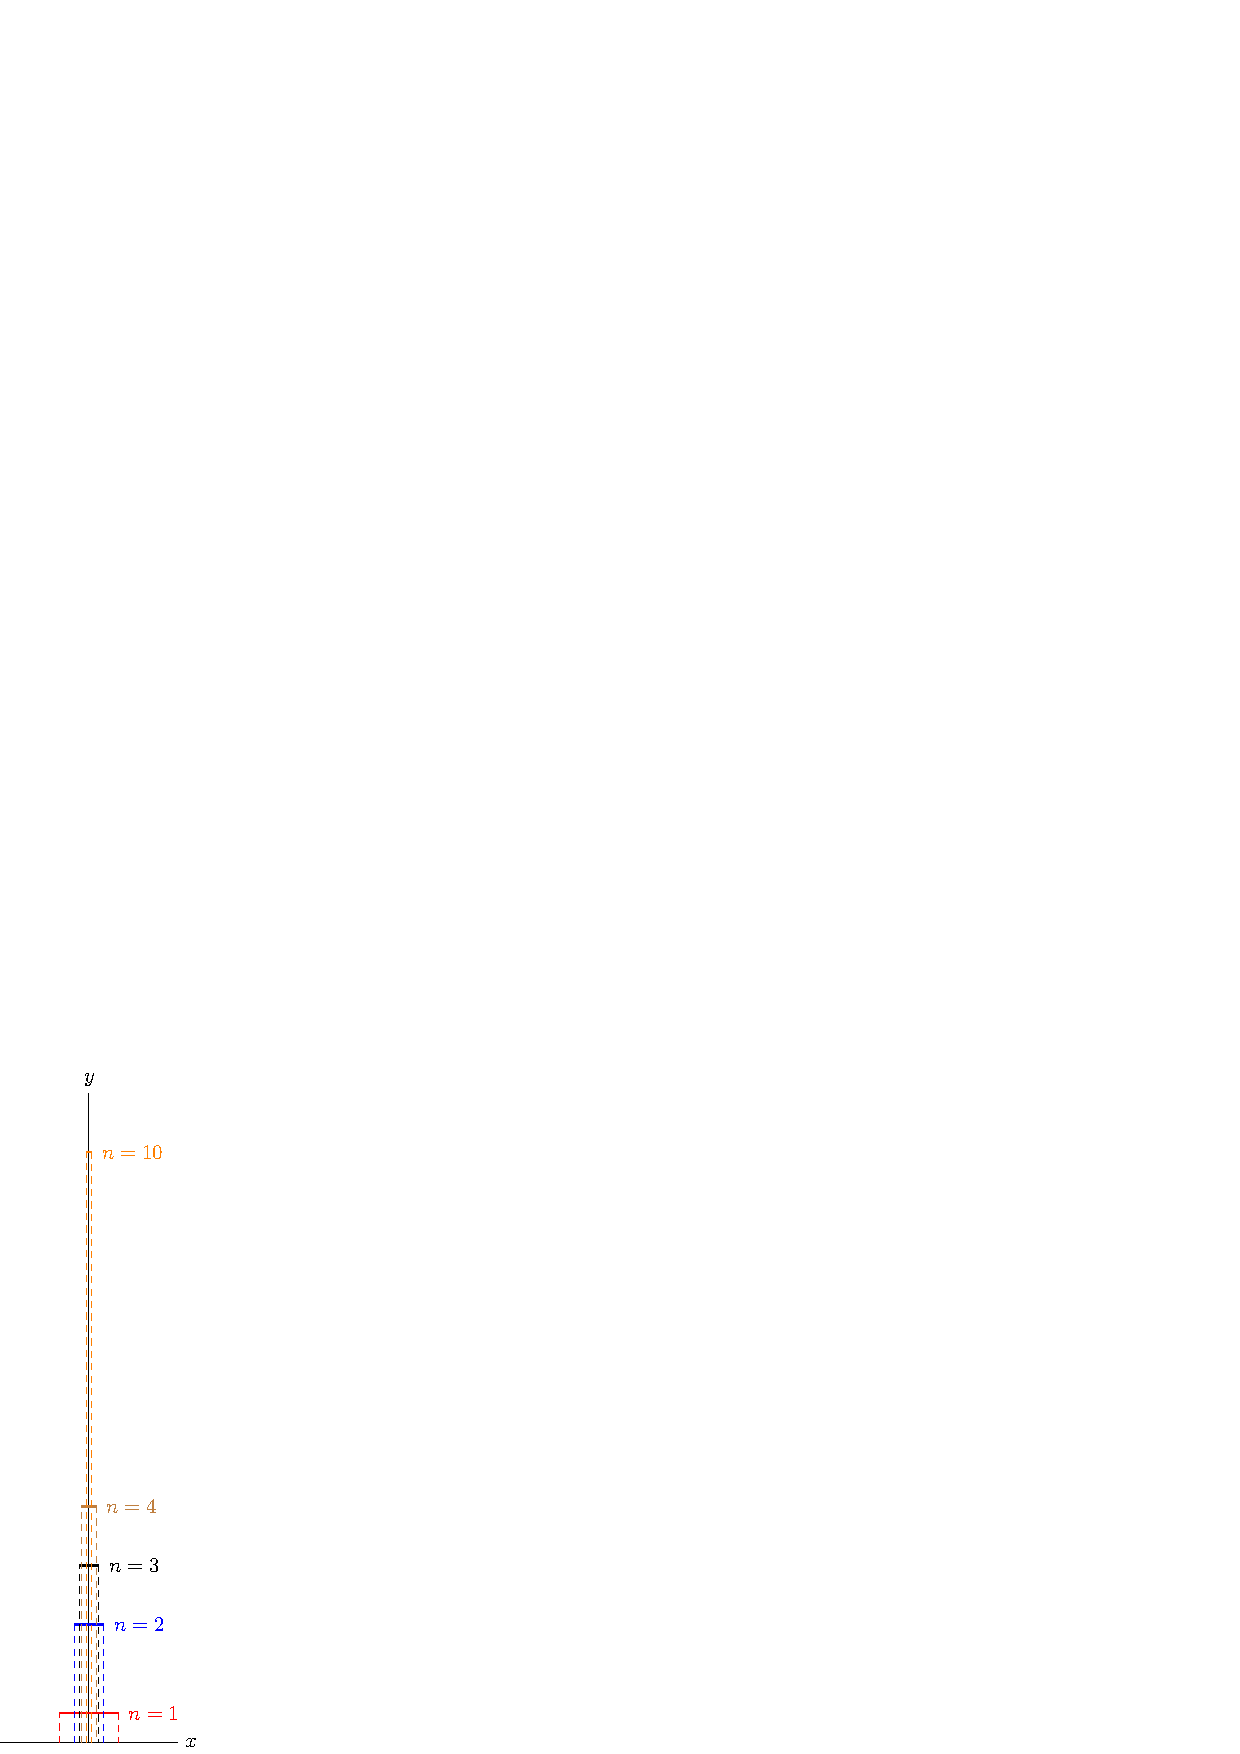
\includegraphics[scale=0.8]{Imagenes/plot_secuencia_delta.pdf}
    \caption{Secuencia delta para valores de $n = 1, 2, \ldots, 10$. El área debajo de la curva para cada $\phi_{n}$ siempre es $1$.}
    \label{fig:secuncia_delta_01}
\end{figure}
Para verificar esta afirmación consideremos la integral
%Apuntes FETI página 46
\begin{align*}
\scaleint{6ex}_{\bs -\infty}^{\infty} \phi_{n} (x) \: f (x) \dd{x}
\end{align*}
para cualquier función continua arbitraria $f (x)$. De la expresión (\ref{eq:ecuacion_delta_04}) para la secuencia delta se tiene
\begin{align*}
\scaleint{6ex}_{\bs -\infty}^{+ \infty} \phi_{n} (x) \: f (x) \dd{x} = \scaleint{6ex}_{\bs -\frac{1}{2 \, n}}^{\frac{1}{2 \, n}} n \: f (x) \: \dd{x} = n \scaleint{6ex}_{\bs -\frac{1}{2 \, n}}^{\frac{1}{2 \, n}} f (x) \:  \dd{x}
\end{align*}
Utilizando el teorema del valor medio para integrales, podemos deducir que
\begin{align*}
n \, \scaleint{6ex}_{\bs -\frac{1}{2 \, n}}^{\frac{1}{2 \, n}} f (x) \dd{x} = n \: \dfrac{1}{n} f (\xi) = f (\xi), \hspace{1cm} - \dfrac{1}{2 \, n} \leq \xi \leq \dfrac{1}{2 \, n}
\end{align*}
En el límite cuando $n \to \infty$, $\xi \to 0$. De la continuidad de la función $f (x)$ se sigue que $f (\xi) \to f (0)$, obteniendo así el resultado
\begin{align*}
\lim_{n \to \infty} \scaleint{6ex}_{\bs -\infty}^{+ \infty} \: \phi_{n} (x) \: f (x) \: \dd{x} = f (0)
\end{align*}
lo que nos dice que la secuencia (\ref{eq:ecuacion_delta_04}), es una secuencia delta.
Nótese que la secuencia delta (\ref{eq:ecuacion_delta_04}) no es derivable en el punto $x = 0$. Para muchos propósitos es deseable construir secuencias delta de funciones que sean continuas y diferenciables. Por ejemplo, en las figuras (\ref{fig:plot_secuencia_01}), (\ref{fig:plot_secuencia_02}) y (\ref{fig:plot_secuencia_03}) podemos apreciar algunas secuencias delta con estas características:
\begin{figure}[H]
    \centering
    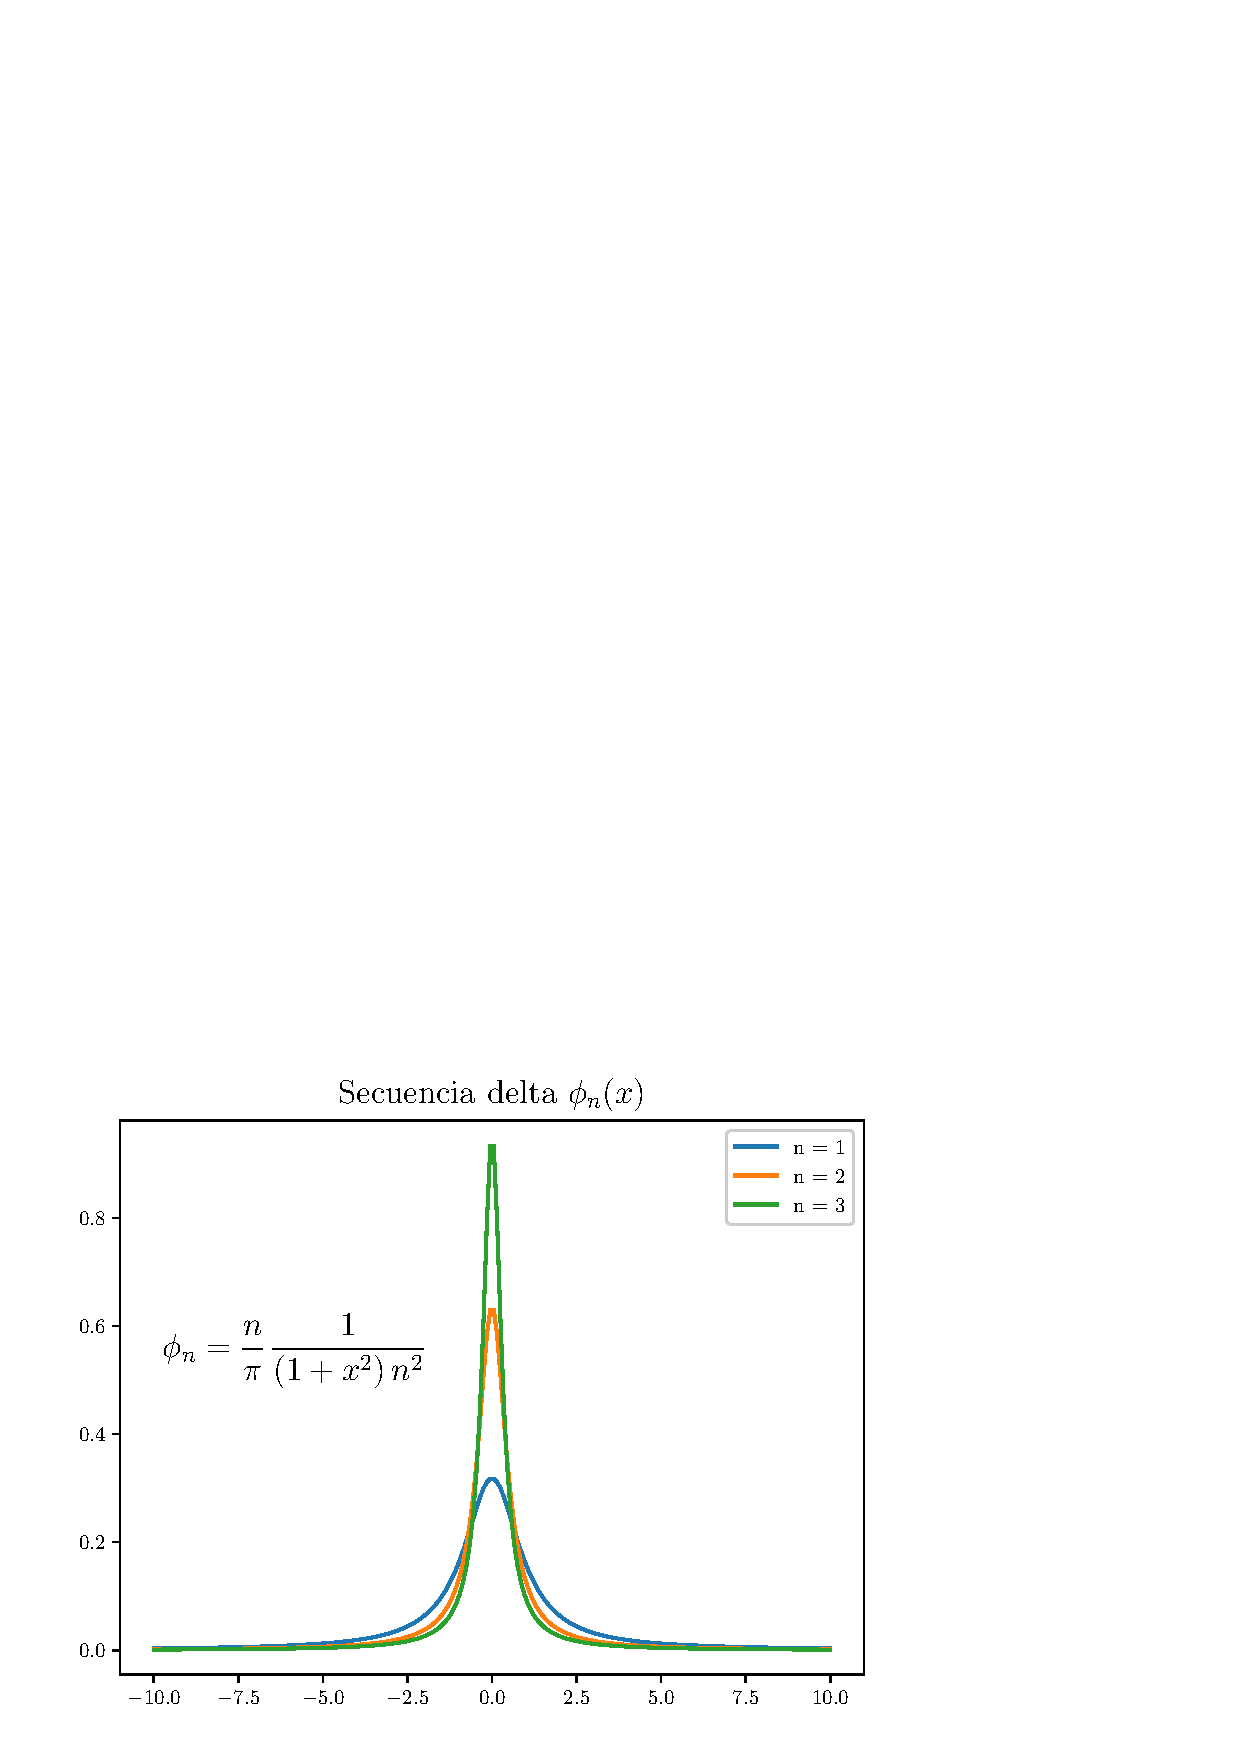
\includegraphics[scale=0.8]{Imagenes/secuencia_delta_01.pdf}
    \caption{Secuencia para $\phi_{n}$ con $n=1,2,3$}
    \label{fig:plot_secuencia_01}
\end{figure}
\begin{figure}[H]
    \centering
    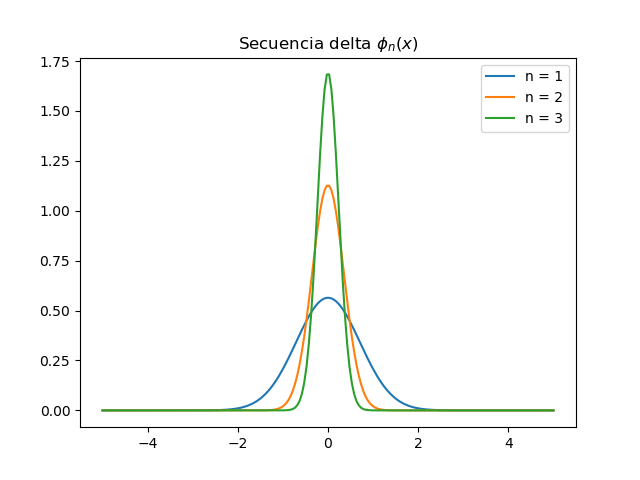
\includegraphics[scale=0.8]{Imagenes/secuencia_delta_02.pdf}
    \caption{Secuencia para $\phi_{n}$ con una función exponencial.}
    \label{fig:plot_secuencia_02}
\end{figure}

\begin{figure}[H]
    \centering
    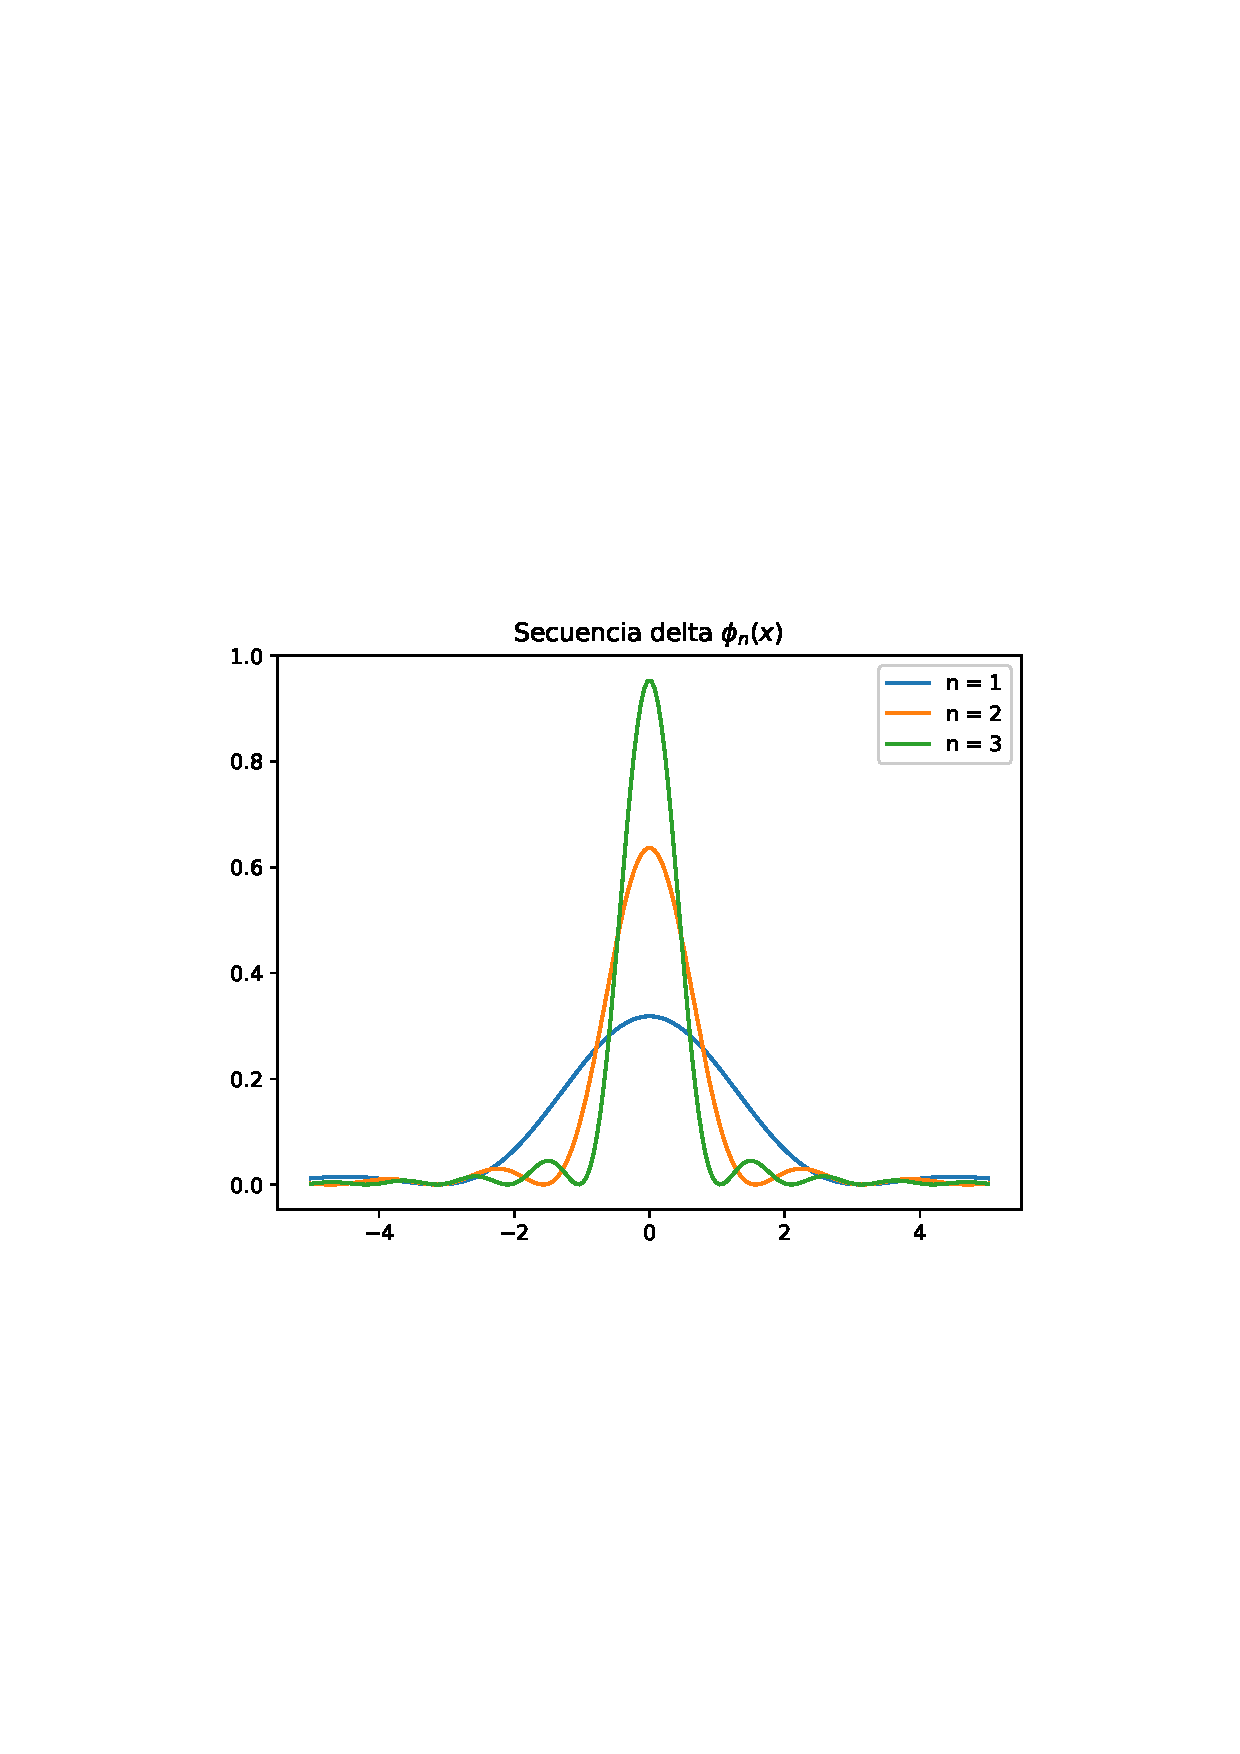
\includegraphics[scale=0.8]{Imagenes/secuencia_delta_03.pdf}
    \caption{Secuencia para $\phi_{n}$ con una función $\sin^{2}(x)/x$}
    \label{fig:plot_secuencia_03}
\end{figure}
Tomemos en cuenta que no es correcto expresar que éstas secuencias convergen a la función delta: los límites de esas secuencias \emph{no existen} (de acuerdo a las definiciones conocidas de convergencia).

Todas estas funciones están normalizadas a la unidad
\begin{equation}
\lim_{n \to \infty} \scaleint{6ex}_{\bs - \infty}^{+ \infty} \phi_{n}(x) \: \dd{x} = 1
\label{eq:ecuacion_delta_05}
\end{equation}

\subsection{Propiedades de la delta de Dirac.}

Una vez que hemos definido la delta de Dirac, nos gustaría saber ahora como operar con y en ella. ¿Es posible decir algo sobre su derivada? La respuesta a esta pregunta es afirmativa y las secuencias delta hechas de funciones diferenciables nos permiten responder a la pregunta de manera precisa.
\par
Por ejemplo, sea la secuencia delta
\begin{align*}
\phi_{n} &= \dfrac{n}{\sqrt{\pi}} e^{-n^{2} x^{2}}
\end{align*}
entonces, al diferenciar la secuencia
\begin{align*}
\dv{\phi_{n}(x)}{x} = - \dfrac{2 \: n^{3}}{\sqrt{\pi}} \: x \: \exp(-n^{2} \: x^{2})
\end{align*}
\begin{figure}[H]
    \centering
    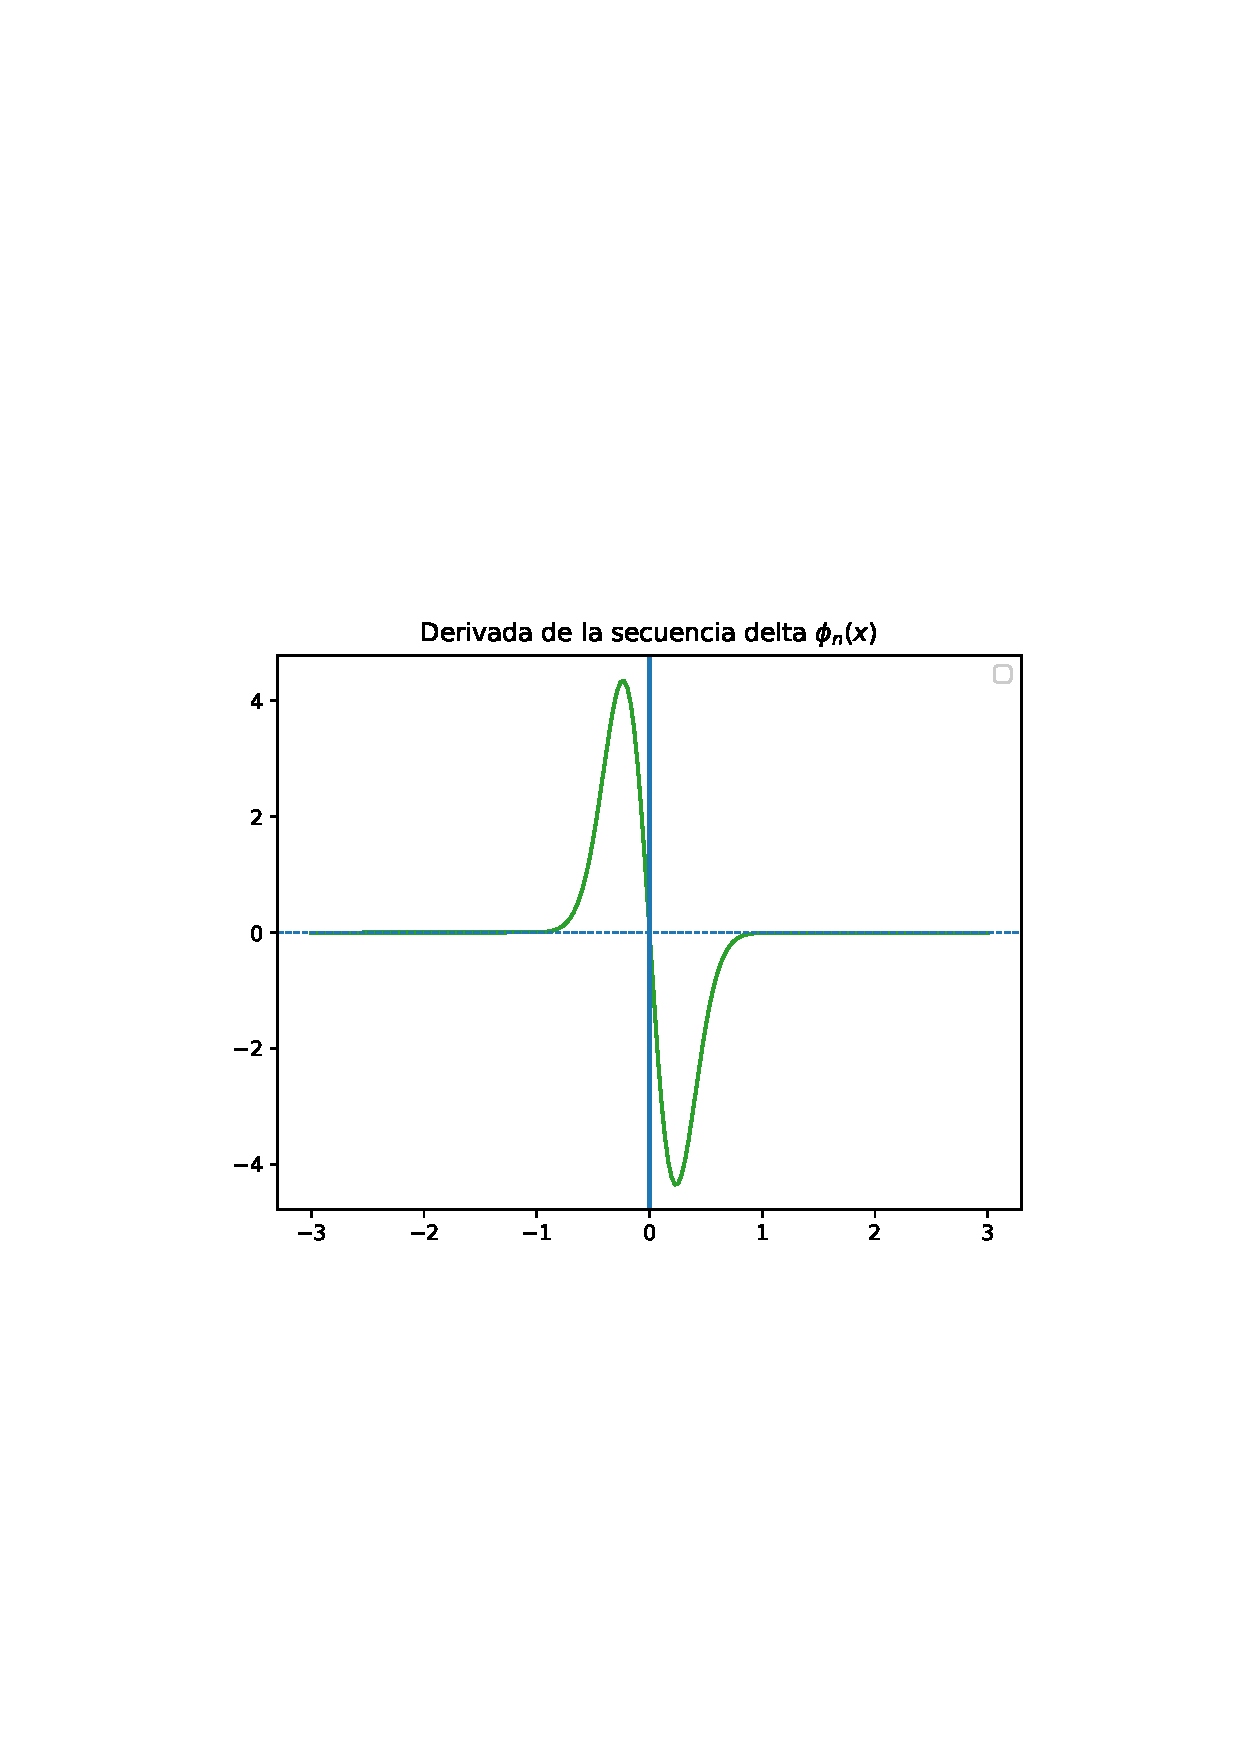
\includegraphics[scale=0.8]{Imagenes/secuencia_delta_04.pdf}
    \caption{Derivada de la secuencia delta.}
    \label{fig:fig_figura_delta_04}
\end{figure}
Consideremos ahora la integral
\begin{align*}
\scaleint{6ex}_{\bs -\infty}^{+\infty} \dv{\phi_{n}(x)}{x} \: f (x) \dd{x}
\end{align*}
donde $f (x)$ es diferenciable. Integrando por partes, se obtiene
\begin{align*}
\scaleint{6ex}_{\bs -\infty}^{+\infty} \dv{\phi_{n}(x)}{x} \: f (x) \dd{x} = \phi_{n} \: f (x) \eval_{-\infty}^{+\infty} - \scaleint{6ex}_{\bs -\infty}^{+\infty} \phi_{n} \: \dv{f (x)}{x} \dd{x}
\end{align*}
Suponemos que
\begin{align*}
\lim_{n \to \infty} \left( \dfrac{n}{\sqrt{\pi}} \right) \exp(-n^{2} \: x^{2}) \: f (x) = 0
\end{align*}
Esto normalmente es cierto, ya que estamos considerando funciones para las cuales la integral
\begin{align*}
\scaleint{6ex}_{\bs -\infty}^{+\infty} \phi_{n}(x) \: f (x) \dd{x} 
\end{align*}
converge.
\par
Entonces, haciendo que $n \to \infty$, tenemos
\begin{align*}
\lim_{n \to \infty} \scaleint{6ex}_{\bs -\infty}^{+\infty} \dv{\phi_{n}(x)}{x} \: f (x) \dd{x} = - \lim_{n \to \infty} \phi_{n}(x) \: f^{\prime} (x) \dd{x} =  -f^{\prime}(0)
\end{align*}
Vemos entonces que la secuencia $\phi^{\prime}(x)$ está relacionada con la propiedad de filtro.
\begin{propiedad}
Propiedad de filtro de las derivadas.
\\
La delta de Dirac satisface la siguiente propiedad:
\[ \scaleint{6ex}_{\bs -\infty}^{+\infty} \dv{\delta(x)}{x} \: f (x) \: \dd{x} = - \dv{f (0)}{x} \]
con $f (x)$ una función diferenciable.
\par
Con la idea anterior, se presenta la propiedad para las derivadas de orden superior de $\delta (x)$:
\begin{align*}
\scaleint{6ex}_{\bs -\infty}^{+\infty} \dv[m]{\delta (x)}{x} \: f (x) \dd{x} =  (-1)^{m} \: \dv[m]{f (0)}{x}
\end{align*}
Es necesario enfatizar que la expresión anterior tiene significado sólo cuando asumimos directamente que las funciones involucradas son $m$ veces diferenciables y que las integrales
\begin{align*}
\scaleint{6ex}_{\bs -\infty}^{+\infty} \dv[k]{\phi_{n}(x)}{x} \: f (x) \dd{x}
\end{align*}
convergen para todo valor de $n$ y para todo valor de $k$ de $0$ a $m$.
\end{propiedad}

La delta de Dirac satisface varias propiedades y conocerlas es de mucha utilidad cuando resolvemos problemas específicos en física. 
\par
\begin{propiedad}
Para el producto de la delta de Dirac con una función se tiene que
\begin{align}
x \: \delta(x) &= 0 \\
f (x) \: \delta(x - a) &= f(a) \: \delta(x - a)
\end{align}
\end{propiedad}
\begin{propiedad}
La paridad de la delta de Dirac y su derivada es
\begin{align}
\delta (-x) &= \delta (x) \\
\delta^{\prime} (-x) &= - \delta^{\prime} (x)
\end{align}
\end{propiedad}
\begin{propiedad}
También satisface las relaciones
\begin{align}
\delta(a \, x) &= \dfrac{1}{\vert a \vert} \: \delta (x), \hspace{1cm} a \neq 0 \\
\delta (x^{2} - a^{2}) &= \dfrac{1}{2 \, a} \left[ \delta (x + a) + \delta (x - a) \right] \hspace{1cm} a > 0
\end{align}
\end{propiedad}
\begin{propiedad}
Las propiedades de filtro
\begin{align}
\scaleint{6ex}_{\bs -\infty}^{\infty} f (x) \: \delta (x - a) \: \dd{x} &= f(a) \\
\scaleint{6ex} \delta (a - x) \: \delta (x - b) \: \dd{x} &= \delta (a - b)
\end{align}
\end{propiedad}

\section{Introduciendo más variables.}

Al introducir más variables:
\begin{equation}
\delta (\va{\bm{r}} - \va{\bm{r_{0}}}) = \delta (x - x_{0}) \: \delta (y - y_{0}) \: \delta (z - z_{0})
\label{eq:ecuacion_A_03}
\end{equation}
de manera que al integrar sobre todo el espacio tenemos
\[ \scaleint{6ex} \delta (\va{\bm{r}} - \va{\bm{r_{0}}}) \: \dd{x} \dd{y}  \dd{z} = 1 \]
\textbf{Ejemplo:}

La función delta permite especificar la densidad de carga debida a un conjunto de $N$ cargas puntuales de valores $q_{i}$ situadas en posiciones $\va{r_{i}}$  como:
\begin{equation}
\rho (\va{r}) = \sum_{i=1}^{N} q_{i} \: \delta(\va{r} - \va{r_{i}})
\label{eq:ecuacion_A_04}
\end{equation}
Las propiedades de la función delta permiten obtener el potencial $\varphi(\va{r})$ evaluando la función dentro de la integral en los puntos $\va{r_{i}}$, es decir
\begin{equation}
\varphi(\va{r}) = \scaleint{6ex} \dfrac{\rho(\va{r^{\prime}})}{\vert \va{r} - \va{r^{\prime}} \vert} \: d^{3}r^{\prime} = \sum_{i=1}^{N} q_{i} \scaleint{6ex} \dfrac{\delta ( \va{r} - \va{r_{i}})}{\vert \va{r} - \va{r^{\prime}} \vert} \: d^{3}r^{\prime} = \sum_{i=1}^{N} \dfrac{q_{i}}{\vert \va{r} - \va{r_{i}} \vert}
\label{eq:ecuacion_A_05}
\end{equation}
Nótese que $\delta (x)$ tiene unidades de inverso de $x$ y $\delta (\va{r})$ tiene unidades de densidad numérica.
\par
La función $\delta$ toma una forma particular en coordenadas cilíndricas y esféricas, dadas por la condición de normalización:
\begin{enumerate}
\item Para coordenadas cilíndricas
\begin{equation}
\scaleint{6ex} \delta (\va{r} - \va{r}_{0}) \: R \: \dd{R} \: \dd{\varphi} \: \dd{z} \Rightarrow \delta (\va{r}) =  \dfrac{1}{R} \: \delta (R - R_{0}) \: \delta (\varphi - \varphi_{0}) \: \delta (z - z_{0})
\end{equation}
\item Para coordenadas esféricas
\begin{equation}
\begin{aligned}
\scaleint{6ex} & \delta (\va{r} - \va{r}_{0}) \: r^{2} \, \dd{r} \, \sin \theta \, \dd{\theta} \, \dd{\varphi} = 1 \\
&\Rightarrow \delta (\va{r}) = \dfrac{1}{r^{2}} \: \delta (r - r_{0}) \, \delta (\cos \theta - \cos \theta_{0}) \, \delta (\varphi - \varphi_{0})
\end{aligned}
\end{equation}
\end{enumerate}
Algunas funciones que en el límite generan la función delta:
\begin{align*}
\delta(x) = \begin{cases}
\displaystyle
\lim_{\varepsilon \to 0^{+}} \dfrac{1}{\pi} \, \dfrac{\varepsilon}{x^{2} + \varepsilon^{2}} & \mbox{Lorentz} \\[1em]
\displaystyle
\lim_{\sigma \to 0^{+}} \dfrac{1}{\sigma \, \sqrt{2 \, \pi}} \, \exp \left( - \dfrac{x^{2}}{2 \, \sigma^{2}} \right) & \mbox{Gaussiana} \\[1em]
\displaystyle \lim_{\varepsilon \to 0^{+}} \dfrac{\sin(x / \varepsilon)}{ \pi \, x} & \mbox{Dirichlet} \\[1em]
\displaystyle \lim_{L \to \infty} \dfrac{1}{2 \, \pi} \scaleint{6ex}_{\bs - \abs{L}}^{\abs{L}} \exp(i \, k \, x) \dd{k} & \mbox{Fourier}
\end{cases}
\end{align*}
%Ref. Farlow (1993) PDE for scientists and engineers. Lesson 1 - Intro to PDE
\section{Ecuaciones diferenciales parciales.}

\subsection{Introducción.}

La mayoría de los fenómenos físicos, ya sea en el dominio de la dinámica de fluidos, la electricidad, el magnetismo, la mecánica clásica o cuántica, la óptica o el flujo de calor, pueden describirse en general mediante \emph{ecuaciones diferenciales parciales} (EDP).
\par
Encontraremos que la mayoría de la física matemática son EDP. Es cierto que se pueden hacer simplificaciones que reduzcan las ecuaciones en cuestión a ecuaciones diferenciales ordinarias, sin embargo, la descripción completa de estos sistemas reside en el área general de las EDP.
\subsection*{Definición.}
Una ecuación diferencial parcial es una ecuación que contiene derivadas parciales. En contraste con las ecuaciones diferenciales ordinarias (EDO), donde la función desconocida depende solo de una variable, en las EDP, la función desconocida depende de varias variables (como la temperatura $u (x, t)$ depende tanto de la posición $x$ como del tiempo $t$).
\par
La representación de una derivada parcial se acostumbra utilizar la notación de Leibniz, como un cociente $\pdv*{u}{t}$, para simplificar la escritura, haremos uso de la siguiente notación tensorial, es decir, con subíndices:
\begin{align*}
\text{\Large{$
u_{t} = \pdv{u}{t} \hspace{1cm} u_{x} = \pdv{u}{x} \hspace{1cm} u_{xx} = \pdv[2]{u}{x} \hspace{1cm} u_{xy} = \pdv[2]{u}{x}{y}$}}
\end{align*}
La forma general de una ecuación diferencial parcial ( EDP) que involucra a dos variables independientes: $x$ e $y$, está dada por:
\begin{align}
F(x, y, \phi_{x}, \phi_{y}, \phi_{xx}, \phi_{yy}, \phi_{xy}, \phi_{xxx}, \phi_{yyy}, \ldots) = 0, \hspace{0.5cm} x, y \in \Omega
\label{eq:ecuacion_B01_01}
\end{align}
donde $\Omega$ es un dominio dado, $F$ es una función con los argumentos que se indican y $\phi$ es una función arbitraria de $(x, y)$. Una solución de la ec. (\ref{eq:ecuacion_B01_01}) corresponde a la función $\phi(x, y)$ que cumple (\ref{eq:ecuacion_B01_01}) para todos los valores de $x$ e $y$.
\par
Si estamos manejando $n$ variables independientes $x_{1}, x_{2}, \ldots, x_{n}$, el dominio $\Omega$ se refiere al espacio n-dimensional que contiene una hipersuperficie $(n-1)$-dimensional. Una hipersuperficie de dimensión $(n-1)$ está dada por la ecuación de la forma $x_{1}^{2} + x_{2}^{2} + \ldots + x_{n}^{2} = 1$ en el espacio Euclidiano n-dimensional.
\par
Veamos de los ejemplos anteriores que la función desconocida $u$ siempre depende de más de una variable. La variable $u$ (que diferenciamos) se llama \textbf{variable dependiente}, mientras que aquellas con respecto a las que diferenciamos se llaman \textbf{variables independientes}. Por ejemplo, de la ecuación
\begin{align*}
\text{\Large{$u_{t} = u_{xx}$}}
\end{align*}
la variable dependiente $u(x, t)$ es una función de dos variables independientes $x$ y $t$; mientras que para la ecuación
\begin{align*}
\text{\Large{$u_{t} = u_{rr} + \dfrac{1}{r} \, u_{r} + \dfrac{1}{r^{2}} \, u_{\theta \theta}$}}
\end{align*}
se tiene que $u(r, \theta, t)$ depende de las variables $r$, $\theta$ y $t$.

\subsection*{¿Por qué son útiles las EDP?}

La mayoría de las leyes naturales de la física, como las ecuaciones de Maxwell, la ley de enfriamiento de Newton, las ecuaciones de Navier-Stokes, las ecuaciones de movimiento de Newton y la ecuación de Schrödinger de la mecánica cuántica, se expresan (o pueden ser expresadas) en términos de EDP, es decir, estas leyes describen los fenómenos físicos relacionando las derivadas espaciales y temporales.
\par
Las derivadas se presentan en estas ecuaciones porque las derivadas modelan cosas naturales (como velocidad, aceleración, fuerza, fricción, flujo, corriente). Por tanto, tenemos ecuaciones que relacionan derivadas parciales de alguna cantidad desconocida que nos gustaría encontrar.

\subsection{¿Cómo se resuelve una ecuación diferencial parcial?}

Esta es una buena pregunta que debemos de plantearnos. Resulta que hay conjunto amplio de métodos disponibles\footnote{Es por esta razón que el nombre de este Tema 2 es: Primeras técnicas de solución, aunque trabajamos con al menos tres técnicas, no implica que sean las únicas, sino que existen otras que se pueden ocupar dependiendo del problema que tengamos que resolver.} para resolver las EDP; los métodos \emph{más importantes son los que convierten las EDP en EDO}, ya que simplifican el manejo y su solución. A continuación mencionamos diez técnicas que son bastante útiles:
\begin{enumerate}
\item \emph{Separación de variables}. Esta técnica reduce una EDP de $n$ variables, a un sistema de $n$ EDO.
\item \emph{Transformadas integrales}. Este procedimiento reduce una EDP de $n$ variables independientes a una de $n - 1$ variables; por lo tanto, una EDP en dos variables podría cambiarse a una EDO.
\item \emph{Cambio de coordenadas}. Este método cambia la EDP original a una EDO o bien a otra EDP (una más fácil) cambiando las coordenadas del problema (rotando el eje o transformaciones similares).
\item \emph{Transformación de la variable dependiente}. Este método transforma la variable incógnita de una EDP en una nueva incógnita que es más fácil de encontrar.
\item \emph{Métodos numéricos}. Estos métodos cambian una EDP a un sistema de ecuaciones en diferencias que puede resolverse mediante un algoritmo con técnicas iterativas en una computadora; en muchos casos, esta es la única técnica que funcionará. Además de los métodos que reemplazan las EDP por ecuaciones en diferencias, existen otros métodos que intentan aproximar soluciones mediante curvas polinomiales (aproximaciones spline).
\item \emph{Métodos de perturbación}. Este método convierte un problema no lineal en una secuencia de problemas lineales que se aproxima al no lineal.
\item \emph{Técnica impulso-respuesta}. Este procedimiento descompone las condiciones iniciales y de frontera del problema en impulsos simples y encuentra la respuesta a cada impulso. La respuesta general se encuentra luego agregando estas respuestas simples.
\item \emph{Ecuaciones integrales}. Esta técnica cambia una EDP a una ecuación integral (una ecuación donde la incógnita está dentro de la integral). Luego, la ecuación integral se resuelve mediante varias técnicas.
\item \emph{Métodos de cálculo de variaciones}. Estos métodos encuentran la solución a las EDP reformulando la ecuación como un problema de minimización. Resulta que el mínimo de cierta expresión (muy probablemente la expresión representará la energía total) también es la solución a la EDP.
\item \emph{Expansión de funciones propias (eigenfunciones)}. Este método intenta encontrar la solución de una EDP como una suma infinita de funciones propias. Estas funciones propias se encuentran resolviendo lo que se conoce como un problema de valores propios correspondiente al problema original.
\end{enumerate}

\subsection{Tipos de EDP.}

Las ecuaciones diferenciales parciales se clasifican de acuerdo a ciertas características que presentan. La clasificación es un concepto importante porque la teoría general y \emph{los métodos de solución generalmente se aplican solo a una clase determinada} de ecuaciones.
\par
A continuación enlistamos seis clasificaciones básicas:
\begin{enumerate}
\item \textbf{Orden de la EDP}. El orden de una EDP es el orden de la derivada parcial más alta, por ejemplo:
\begin{table}[H]
\centering
\large
\begin{tabular}{l l}
\Large{$u_{t} = u_{xx}$} & es de segundo orden \\
\Large{$u_{t} = u_{x}$} & es de primer orden \\
\Large{$u_{t} = u \, u_{xxx} + \sin x$} & es de tercer orden
\end{tabular}
\end{table}

\item \textbf{Número de variables}. El número de variables es el número de variables independientes, por ejemplo:
\begin{table}[H]
\centering
\large
\begin{tabular}{l l}
\Large{$u_{t} = u_{xx}$} & dos variables: $x, t$ \\
\Large{$u_{t} = u_{rr} + \dfrac{1}{r} \, u_{r} + \dfrac{1}{r^{2}} \, u_{\theta \theta}$} & tres variables: $r, \theta, t$
\end{tabular}
\end{table}
\item \textbf{Linealidad}. Las EDP son lineales o no lineales. En las lineales, la variable dependiente $u$ y todas sus derivadas aparecen de forma lineal (no se multiplican juntas ni al cuadrado, por ejemplo). Más precisamente, una \emph{ecuación lineal de segundo orden en dos variables} es una ecuación de la forma
\begin{align}
\addtolength{\fboxsep}{5pt}\boxed{ A \, u_{xx} + B \, u_{xy} + C \, u_{yy} + D \, u_{x} + E \, u_{y} + F \, u = G}
\label{eq:ecuacion_01_01}
\end{align}
donde $A, B, C, D, E, F$ y $G$ pueden ser \emph{constantes} o \emph{funciones de} $(x, y)$, por ejemplo
\begin{table}[H]
\centering
\large
\begin{tabular}{l p{1cm} l}
\Large{$e^{-t} \, u_{xx} + \sin t = u_{tt}$} & & lineal \\
\Large{$u \, u_{xx} + u_{t} = 0$} & & no lineal \\
\Large{$u_{xx} + y \, u_{yy} = 0$} & & lineal \\
\Large{$x \, u_{x} + y \, u_{y} + u^{2} = 0$} & & no lineal
\end{tabular}
\end{table}
\item \textbf{Homogeneidad}. La ec. (\ref{eq:ecuacion_01_01}) se denomina \emph{homogénea} si el lado derecho de la igualdad $G(x, y)$ es cero para todo $x$, e $y$. Mientras que si $G(x, y)$ no se anula, entonces la ecuación se denomina \emph{no homogénea}.
\item \textbf{Tipo de coeficientes}. Si los coeficientes $A, B, C, D, E, F$ en la ec. (\ref{eq:ecuacion_01_01}) son constantes, entonces (\ref{eq:ecuacion_01_01}) tiene \emph{coeficientes constantes}, de otra manera, la ecuación tiene \emph{coeficientes variables}.
\item \textbf{Tres tipos de ecuaciones lineales}. Toda EDP lineal como la ec. (\ref{eq:ecuacion_01_01}) puede clasificarse como de tipo:
\begin{enumerate}[label=(\alph*)]
\item Parabólico.
\item Hiperbólico.
\item Elíptico.
\end{enumerate}
Las ecuaciones \textbf{parabólicas} describen por ejemplo el flujo de calor y procesos de difusión, además satisfacen la propiedad $B^{2} - 4 \, A \, C = 0$.
\par
Las ecuaciones \textbf{hiperbólicas} describen sistemas que vibran así como el movimiento de las ondas, satisfacen la propiedad $B^{2} - 4 \, A \, C > 0$.
\par
Las ecuaciones \textbf{elípticas} describe fenómenos estacionarios y satisfacen la propiedad $B^{2} - 4 \, A \, C < 0$.
\par
Como ejemplo veamos:
\begin{table}[H]
\centering
\large
\begin{tabular}{c l l l l l}
(a) & \Large{$u_{t} = u_{xx}$} & & \large{$B^{2} - 4 \, A \, C = 0$} & & parabólica \\
(b) & \Large{$u_{tt} = u_{xx}$} & & \large{$B^{2} - 4 \, A \, C = 4$} & & hiperbólica \\
(c) & \Large{$u_{\xi \eta} = 0$} & & \large{$B^{2} - 4 \, A \, C = 1$} & & hiperbólica \\
(d) & \Large{$u_{xx} + u_{yy} = 0$} & & \large{$B^{2} - 4 \, A \, C = -4$} & & elíptica \\
(e) & \Large{$y \, u_{xx} + u_{yy} = 0$} & & \large{$B^{2} - 4 \, A \, C = - 4 \, y$} & & \\
 & & & es $\begin{cases}
    \mbox{elíptica para } y > 0 \\
    \mbox{parabólica para } y = 0 \\
    \mbox{hipérbolica para } y < 0 \\
    \end{cases}$ &
\end{tabular}
\end{table}
En el caso de coeficientes variables, el tipo de ecuación cambia de punto a punto.
\end{enumerate}

\subsection*{Consideraciones}
\begin{enumerate}
\item En general, $B^{2} - 4 \, A \, C$ es una función de las variables independientes; por lo tanto, una ecuación puede cambiar de un tipo básico a otro en todo el dominio de la ecuación (aunque no es común).
\item La ecuación lineal general (\ref{eq:ecuacion_01_01}) se escribió con variables independientes $x$ e $y$. En muchos problemas, una de las dos variables representa el tiempo, por lo tanto, se escribiría en términos de $x$ y $t$.
\item En la figura (\ref{fig:figura_clasificacion_EDP}) se muestra un diagrama de clasificación general:
\begin{figure}[H]
    \centering
    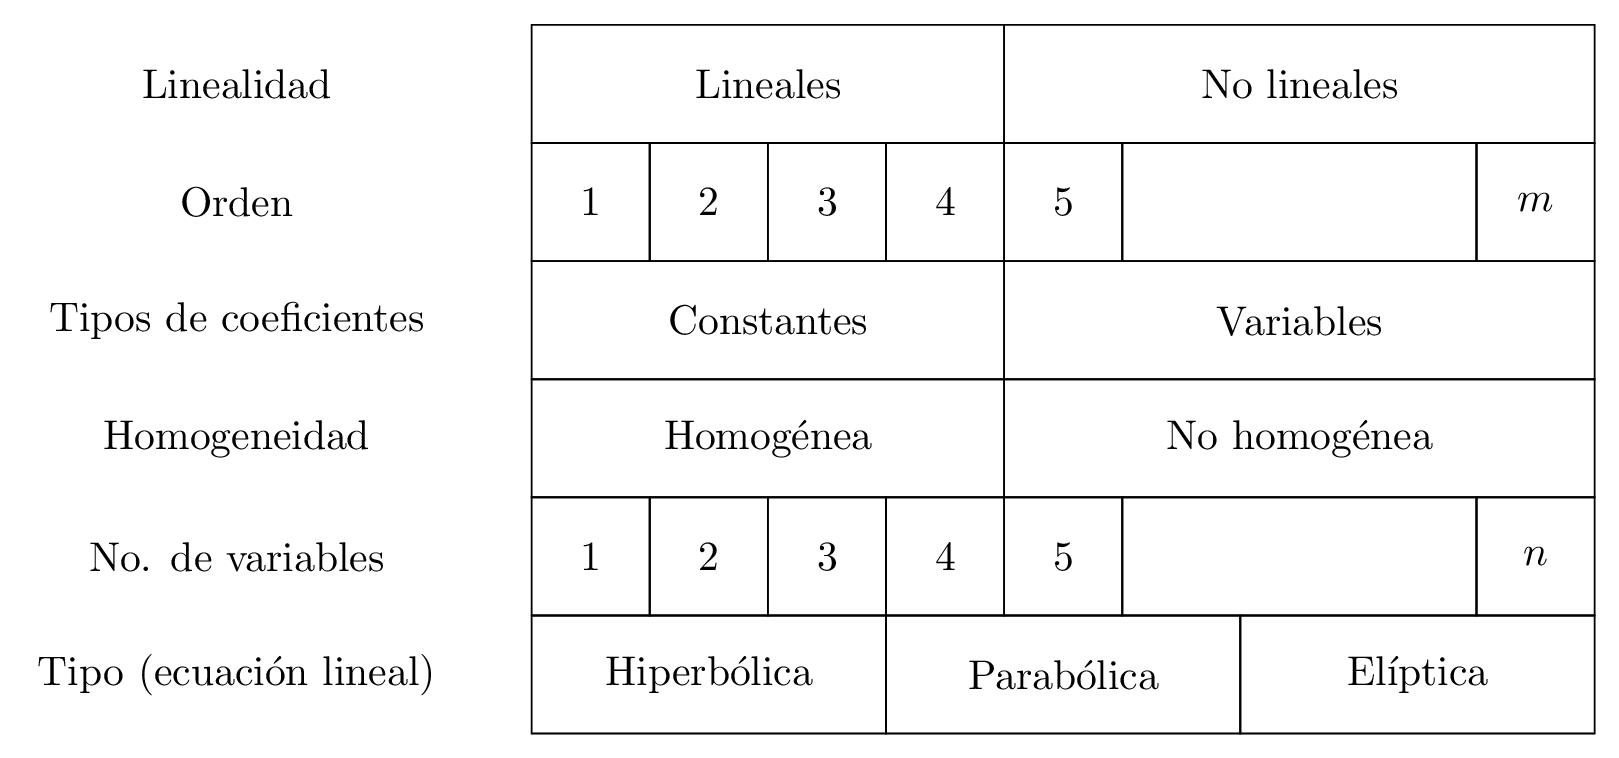
\includegraphics[scale=0.25]{Imagenes/Cuadro_Clasificacion_EDP.png}
    \caption{Diagrama de clasificación de EDP.}
    \label{fig:figura_clasificacion_EDP}
\end{figure}
\end{enumerate}

%Ref. Zamora (2012) . Notas EDP 1.1.3 Problemas asociados.
\section{Problemas asociados.}

Se denomina un \emph{problema} a la EDP junto con un conjunto de condiciones dadas. Suponiendo una ecuación de la forma:
\begin{align}
F(x, t, u, u_{x}, u_{t}, u_{xx}, u_{xt}, u_{tt}) = 0
\label{eq:ecuacion_Z01_06}
\end{align}
es decir, una EDP de segundo orden en dos variables, se definen los distintos problemas.

\subsection{Problema de Cauchy.}
Este problema se conoce también como \emph{problema de valores iniciales}. Dado el carácter de segundo orden en las derivadas respecto al tiempo $t$ de la ec. (\ref{eq:ecuacion_Z01_06}, son necesarias dos condiciones sobre la solución $u(x, t)$. Estas son:
\begin{align}
u(x, 0) &= \phi (x) \label{eq:ecuacion_Z01_07} \\[0.5em]
u_{t}(x, 0) &= \psi (x) \label{eq:ecuacion_Z01_08}
\end{align}
donde $\phi$ y $\psi$ son funciones dadas en el intervalo de interés, y se ha elegido el tiempo inicial $t = 0$.
\par
Nótese que si en la EDP el orden mayor de la derivada respecto a $t$ fuese $N,$ entonces serían necesarias las derivadas parciales de $u$ respecto a $t$ desde el orden $0$ hasta el $N - 1$ evaluadas al tiempo $t = 0$ como condiciones.

\subsection{Problema de Dirichlet.}

Este es un tipo de problema conocido como de valores en la frontera. Dado el carácter de segundo orden en las derivadas respecto a la posición $x$ de la ec. (\ref{eq:ecuacion_Z01_06}), se necesitan dos condiciones sobre la solución $u(x, t)$. Suponiendo que se busca la solución para $a  \leq x \leq b$, $t \geq 0$, éstas son:
\begin{align}
u(a, t) &= f (t) \label{eq:ecuacion_Z01_09} \\[0.5em]
u(b, t) &= g(t) \label{eq:ecuacion_Z01_10}
\end{align}
donde $f$ y $g$ son funciones dadas, definidas para $t \geq 0$.
\par
Ahora notemos que si en la EDP el orden mayor de la derivada respecto a $x$ fuese $N$, entonces serían necesarios los valores de $u$ en $N$ distintos $x = a_{i}$ como condiciones. De manera general, el problema de Dirichlet \emph{prescribe} el valor de la función incógnita, $u$, en toda la \emph{frontera} de la región de interés.

\subsection{Problema de Neumann.}

Este es otro tipo de problema de \emph{valores en la frontera}. Suponiendo que se busca la solución para $a \leq x \leq b$, $t \geq 0$, las condiciones son en este caso las siguientes:
\begin{align}
u_{x}(a, t) &= f(t) \label{eq:ecuacion_Z01_11} \\[0.5em]
u_{x}(b, t) &= g(t) \label{eq:ecuacion_Z01_12}
\end{align}
donde $f$ y $g$ son funciones dadas, definidas para $t \geq 0$.
\par
Revisemos que si en la EDP el orden mayor de la derivada respecto a $x$ fuese $N$, entonces serían necesarios los valores de $u_{x}$ en $N$ distintos $x = a_{i}$ como condiciones. De manera general, el problema de Neumann \emph{prescribe} el valor de la derivada normal de la función incógnita, $\pdv*{u}{n}$, en toda la \emph{frontera} de la región de interés.

\subsection{Problema de Robin.}

Este problema \emph{de valores en la frontera} generaliza los dos anteriores. Suponiendo que se busca la solución para $a \leq x \leq b$, $t \geq 0$, las condiciones son:
\begin{align}
A_{1} \, u(a, t) + B_{1} \, u_{x}(a, t) &= f(t) \label{eq:ecuacion_Z01_13} \\[0.5em]
A_{2} \, u(b, t) + B_{2} \, u_{x}(b, t) &= g(t) \label{eq:ecuacion_Z01_14}
\end{align}
donde $f$ y $g$ son funciones dadas, definidas para $t \geq 0$, y $A_{1}, B_{1}, A_{2} y B_{2}$ son constantes dadas.
\par
Vale la pena remarcar que si en la EDP el orden mayor de la derivada respecto a $x$ fuese $N$, entonces serían necesarios los valores de $u$ y $u_{x}$ en $N$ distintos $x = a_{i}$ como condiciones. De manera general, el problema de Robin \emph{prescribe} el valor de una combinación lineal de la función incógnita $u$ y su derivada normal $\pdv*{u}{n}$ en toda la \emph{frontera} de la región de interés.

\subsection{Problemas Mixtos.}

Son problemas \emph{de valores en la frontera} y/o iniciales que mezclan condiciones de los anteriores. Suponiendo que se busca la solución para $a \leq x \leq b$, $t \geq 0$, un ejemplo sería el siguiente:
\begin{align}
A_{1} \, u(a, t) + B_{1} \, u(b, t) &= f(t) \label{eq:ecuacion_Z01_15} \\[0.5em]
A_{2} \, u_{x}(a, t) + B_{2} \, u_{x}(b, t) &= g(t) (\label{eq:ecuacion_Z01_16}
\end{align}
donde $f$ y $g$ son funciones dadas, definidas para $t \geq 0$, y $A_{1}, B_{1}, A_{2} y B_{2}$ son constantes dadas.
\par
Notemos que si en la EDP el orden mayor de la derivada respecto a $x$ fuese $N$, entonces serían necesarios los valores de $u$ o $u_{x}$ en $N$ distintos $x = a_{i}$ como condiciones. De manera general, los problemas mixtos \emph{prescriben} valores de combinaciones lineales de la función incógnita $u$ (o de su derivada normal $\pdv*{u}{n}$) evaluada en distintas partes de la \emph{frontera} de la región de interés.

\section{Problemas bien definidos.}

Se dice que un problema matemático que involucra EDP está \emph{bien definido} (o planteado) si satisface los siguientes requisitos:
\begin{enumerate}
\item Existencia: hay al menos una solución.
\item Unicidad: hay como máximo una solución.
\item Estabilidad: La solución depende continuamente de los datos.
\end{enumerate}

El primer requisito es una condición lógica obvia, pero debemos tener en cuenta que no podemos simplemente afirmar que el problema matemático tiene una solución solo porque el problema físico tiene una solución. Bien podemos estar desarrollando erróneamente un modelo matemático, digamos, que consiste en una EDP cuya solución puede no existir en absoluto. Lo mismo puede decirse del requisito de unicidad. Para reflejar realmente el problema físico que tiene una solución única, el problema matemático debe tener una solución única.
\par
Para problemas físicos, no es suficiente saber que el problema tiene una solución única. Por lo tanto, el último requisito no solo es útil sino también esencial. Para que la solución tenga importancia física, un pequeño cambio en los datos iniciales debe producir un pequeño cambio en la solución. Los datos de un problema físico se obtienen normalmente de experimentos y se aproximan para resolver el problema por métodos numéricos o aproximados. Es fundamental saber que el proceso de hacer una aproximación a los datos produce solo un pequeño cambio en la solución.

%Ref. http://www.scholarpedia.org/article/Partial_differential_equation
\section{Ecuaciones en la Física Matemática.}

\subsection{Ecuaciones lineales.}
Enumeremos algunas EDP conocidas:
\begin{enumerate}
    \item La ecuación de calor (ecuación parabólica)
\begin{align}
\text{\Large{$u_{t} - u_{xx} = 0$}}
\label{eq:ecuacion_S11}
\end{align}
donde las variables $t$ y $x$ juegan el papel de tiempo y una coordenada espacial, respectivamente. Revisemos que  en cuenta que la ecuación (\ref{eq:ecuacion_S11}) contiene solo un término con una derivada más alta.
\par
La ecuación (\ref{eq:ecuacion_S11}) se encuentra a menudo en la teoría de la transferencia de calor y de masa. Describe procesos térmicos inestables unidimensionales en medios inactivos o sólidos con difusividad térmica constante. Se utiliza una ecuación similar para estudiar los correspondientes procesos de intercambio de masa inestables unidimensionales con difusividad constante.
\item La ecuación de onda (ecuación hiperbólica)
\begin{align}
\text{\Large{$u_{tt} - u_{xx} = 0$}}
\label{eq:ecuacion_S12}
\end{align}
donde las variables $t$ y $x$ juegan el papel del tiempo y la coordenada espacial, respectivamente. Revisemos que los términos de la derivada más alta en la ecuación (\ref{eq:ecuacion_S12}) difieren en un signo.
\par
Esta ecuación también se conoce como \emph{ecuación de vibración de una cuerda}. A menudo se encuentra en elasticidad, aerodinámica, acústica y electrodinámica.
\item Ecuación de Laplace (ecuación elíptica)
\begin{align}
\text{\Large{$u_{xx} + u_{yy} = 0$}}
\label{eq:ecuacion_S14}
\end{align}
donde $x$ e $y$ juegan el papel de las coordenadas espaciales. Tomemos en cuenta que los términos de la derivada más alta en la ecuación (\ref{eq:ecuacion_S14}) tienen signos similares. La ecuación de Laplace a menudo se escribe brevemente como $\laplacian{u} = 0$, donde $\laplacian$ es el operador de Laplace o laplaciano.
\par
La ecuación de Laplace se encuentra a menudo en la teoría de transferencia de calor y masa, mecánica de fluidos, elasticidad, electrostática y otras áreas de la mecánica y la física. Por ejemplo, en la teoría de transferencia de calor y masa, esta ecuación describe la distribución de temperatura en estado estable en ausencia de fuentes de calor y sumideros en el dominio en estudio.
\end{enumerate}
\subsection{Ecuaciones no lineales.}
\begin{enumerate}
\item Ecuación no lineal de calor:
\begin{align}
\pdv{u}{t} = \pdv{x} \left[ f(u) \, \pdv{u}{x} \right]
\label{eq:ecuacion_S27}  
\end{align}
Esta ecuación describe procesos térmicos inestables unidimensionales en medios o sólidos en reposo en el caso en que la difusividad térmica depende de la temperatura, $f (u)> 0$. En el caso especial $f (w) \equiv 1$, la ecuación no lineal (\ref{eq:ecuacion_S27}) se convierte en la ecuación de calor lineal (\ref{eq:ecuacion_S11}).
\item Ecuación Kolmogorov-Petrovskii-Piskunov:
\begin{align}
\pdv{u}{t} = a \, \pdv[2]{w}{x} + f(u), \hspace{1cm} a > 0
\label{eq:ecuacion_S28}
\end{align}
Las ecuaciones de esta forma se encuentran a menudo en varios problemas de transferencia de masa y calor (siendo $f$ la reacción de cambio del volumen en una reacción química), teoría de la combustión, biología y ecología.
\par
En el caso especial de $f (u) \equiv 0$ y $a = 1$, la ecuación no lineal (\ref{eq:ecuacion_S28}) se convierte en la ecuación de calor lineal (\ref{eq:ecuacion_S11}).
\par
Observación: La ecuación (\ref{eq:ecuacion_S28}) también se le conoce como \emph{ecuación de calor con una fuente no lineal}.
\item Ecuación de Burgers:
\begin{align}
\pdv{w}{t} + u \, \pdv{u}{x} = \pdv[2]{u}{x}
\label{eq:ecuacion_S29}
\end{align}
Se ocupa para describir procesos ondulatorios en la dinámica de gases, hidrodinámica, en acústica y para el flujo del tráfico.
\item Ecuación de onda no lineal:
\begin{align}
\pdv[2]{u}{t} = \pdv{x} \left[ f(u) \, \pdv{u}{x} \right]
\label{eq:ecuacion_S30}
\end{align}
Esta ecuación se encuentra en dinámica de ondas y gases, con $f(u) > 0$. En el caso especial $f(u) \equiv 1$, la ecuación no lineal (\ref{eq:ecuacion_S30}) pasa a ser la ecuación de onda lineal (\ref{eq:ecuacion_S12}).
\item Ecuación Klein-Gordon no lineal:
\begin{align}
\pdv[2]{u}{t} = a \, \pdv[2]{u}{x} + f(u),\hspace{1cm} a > 0
\label{eq:ecuacion_S31}
\end{align}
Las ecuaciones de esta forma surgen en geometría diferencial y diversas áreas de la física: superconductividad, dislocaciones en cristales, ondas en materiales ferromagnéticos, pulsos de láser en medios bifásicos, entre otros. Para $f (u) \equiv 0$ y $a = 1$, la ecuación coincide con la ecuación de onda lineal.
\item Ecuación de Laplace no lineal:
\begin{align}
\pdv[2]{u}{x} + \pdv[2]{u}{y} = f(u)
\label{eq:ecuacion_S32}
\end{align}
A esta ecuación se le conoce también como \emph{ecuación estacionaria de calor con una fuente no lineal.}
\item Ecuación Monge-Ampere:
\begin{align}
\left( \pdv[2]{u}{x}{y} \right)^{2} - \pdv[2]{u}{x} \, \pdv[2]{u}{y} = (x, y)
\label{eq:ecuacion_S33}
\end{align}
Esta ecuación se encuentra en geometría diferencial, dinámica de gases y meteorología.
\end{enumerate}

\subsection{Ecuaciones lineales de derivadas de orden mayor.}

\begin{enumerate}
\item Ecuación de vibración de un varilla elástica:
\begin{align*}
\pdv[2]{w}{t} + a^{2} \, \pdv[4]{u}{x} = 0
\end{align*}
\item La ecuación biarmónica
\begin{align*}
\nabla^{4} = 0
\end{align*}
donde $\nabla^{4}$ es el operador biarmónico:
\begin{align*}
\nabla^{4} = \pdv[4]{x} + 2 \, \dfrac{\partial^{4}}{\partial x^{2} \, \partial y^{2}} + \pdv[4]{u}{y}
\end{align*}
La ecuación biarmónica se encuentra en problemas bidimensionales de elasticidad (como la función de tensión de Airy). También se utiliza para describir flujos lentos de fluidos viscosos incompresibles ($u$ es la función de corriente).
\end{enumerate}
Las ecuaciones que se han mencionado no son todas en la física matemática, habrá otras ecuaciones que extenderán este listado. Dependiendo del área de interés que decidas abordar, lo más seguro es que te encuentres con nuevas ecuaciones, que esperamos logres identificar las características principales, así como un abordaje para su solución. En el siguiente material de trabajo se revisará la técnica de solución: \emph{separación de variables.}
\section{Ecuaciones diferenciales parciales.}

Una vez que se ha realizado la formulación de una EDP el siguiente paso es resolver la ecuación, en un primer momento podemos considerar la solución general de la EDP, entonces en vez de constantes arbitrarias aparecen funciones arbitrarias.
\par
Por ejemplo, la solución general de $u_{xy} = 0$ es 
\begin{align*}
u (x, y) = G (x) + F (y)
\end{align*}
donde $G$, $F$ son funciones arbitrarias.
\par
Dado que se quieren resolver problemas específicos, hay que estudiar el tipo de condiciones que hay que imponer para garantizar \emph{la unicidad} de la solución. Como se revisó en la presentación anterior, tenemos una clasificación con tres tipos de ecuaciones (parabólica, hiperbólica y elíptica) a continuación presentamos un posible tipo de condiciones de frontera (CDF) que se pueden presentar.

\subsection{EDP Parabólica.}

Consideremos la ecuación del calor
\begin{align*}
u_{t} =  \alpha^{2} \,  u_{xx}
\end{align*}
En este caso se trabajará con un problema unidimensional, es decir, la transmisión del calor a lo largo de una barra de longitud $L$.
\par
Para que el problema tenga solución se debe de especificar la distribución inicial de temperatura de la barra, es decir, hay que dar una función $\varphi (x)$ de modo que
\begin{align}
u (x, 0) = \alpha (x) \hspace{1.5cm} \text{distribución inicial de temperatura}
\label{eq:ecuacion_06_02_02}
\end{align}
que en analogía con las EDO, tiene sentido llamar tal condición una \emph{condición inicial}.
\par
A su vez, como la barra tiene una longitud finita, hay que especificar la interacción de los extremos de la barra con el medio ambiente. Tales condiciones se conocen como \emph{condiciones de frontera}.
\par
Para los problemas de una dimensión hay tres tipos de condiciones de frontera usuales, aunque solo se estudiarán las primeras dos en esta revisión:
\begin{enumerate}
\item \textbf{Condición de Dirichlet}: Consiste en especificar la temperatura en los extremos de la barra en todo instante, es decir, dar dos funciones $f (t)$ y $g (t)$ de modo que:
\begin{align}
u (0, t) = f (t)  \hspace{1cm} u (L, t) = g (t) \hspace{1cm} \text{condiciones tipo Dirichlet}
\label{eq:ecuacion_06_02_03}    
\end{align}
\item \textbf{Condición de Neumann}: Consiste en especificar la derivada de la temperatura en los extremos de la barra, es decir, especificar el flujo de calor en los extremos de la barra:
\begin{align}
u_{x} (0, t) = f (t) \hspace{1cm} u_{x} (L, t) = g (t) \hspace{1cm} \text{condiciones tipo Neumann}
\label{eq:ecuacion_06_02_04}    
\end{align}
\item \textbf{Condiciones mixtas (de Robin)}: Consiste en especificar una combinación de $u$ y de $u_{x}$ en los extremos de la barra.
\end{enumerate}

\subsection{EDP Elíptica.}

Sea la ecuación de Laplace:
\begin{align*}
u_{xx} + u_{yy} = 0
\end{align*}
Se puede interpretar como la ecuación de un potencial electrostático sobre una región del plano $xy$ o bien la distribución de temperatura en el caso estacionario para una placa o una región del plano $xy$.
\par
En este caso no hay que especificar condiciones iniciales pues la función no depende del tiempo. Se estudiarán dos tipos de condiciones:
\begin{enumerate}
\item \textbf{Condición de Dirichlet}: Si se trabaja sobre una lámina rectangular $0 < x < a$ y $0 < y < b$ las condiciones de Dirichlet consisten en especificar los valores de la temperatura (o el potencial) sobre todos los lados, es decir:
\begin{align}
\begin{aligned}
u (0, y) &= f_{1} (y) \hspace{1.5cm} u (a, y) = f_{2} (y) \\
u (x, 0) &= g_{1} (x) \hspace{1.5cm} u (x, b) = g_{2} (x)
\end{aligned}
\label{eq:ecuacion_06_02_05}
\end{align}
\item \textbf{Condiciones Mixtas}: Para los lados de la placa se toman dos de las condiciones de Dirichlet y las otras dos de Neumann, por ejemplo:
\begin{align}
\begin{aligned}
u_{y} (0, y) &= f_{1} (y) \hspace{1.5cm} u_{y} (a, y) = f_{2} (y) \\
u (x, 0) &= g_{1} (x) \hspace{1.5cm} u (x, b) = g_{2} (x)
\end{aligned}
\label{eq:ecuacion_06_01_06}
\end{align}
\end{enumerate}

\subsection{EDP Hiperbólica.}

La ecuación de onda
\begin{align*}
u_{tt} = v^{2} \, u_{xx}
\end{align*}
En este caso se considera una cuerda de longitud $L$. Como la ecuación es de segundo orden en el tiempo, tiene sentido esperar que haya que especificar la posición inicial de la cuerda así como su velocidad inicial, es decir, proporcionar:
\begin{align}
u (x, 0) = \phi (x) \hspace{1.5cm} u_{t} (x, 0) = \psi (x) \hspace{1cm} \mbox{condiciones iniciales}
\label{eq:ecuacion_06_02_07}
\end{align}
a su vez, hay que especificar como se relaciona la cuerda con su frontera y nuevamente se van a estudiar las condiciones de Dirichlet y de Neumann.
\begin{enumerate}
\item \textbf{Condición de Dirichlet}: Se especifica la posición de los extremos de la cuerda, es decir:
\begin{align}
u (0, t) = f (t) \hspace{1.5cm} u (L, t) = g (t)
\label{eq:ecuacion_06_02_08}   
\end{align}
\item \textbf{Condición de Neumann}: Se especifica la forma en que se están \enquote{jalando} los extremos de la cuerda, es decir:
\begin{align}
u_{x} (0, t) = f (t) \hspace{1.5cm} u_{x} (L, t) = g (t)
\label{eq:ecuacion_06_02_09}    
\end{align}
\end{enumerate}
Como se veremos más adelante, el \emph{método de separación de variables} consiste en suponer que la solución depende como un producto de funciones, cada una de las cuales depende exclusivamente de una de las variables independientes.
\par
Para que tenga éxito el método, se ocupará que varias de las condiciones de frontera estén igualadas a cero, de forma que se utilicen para restringir las soluciones a las ecuaciones diferenciales ordinarias que aparecen.
\par
Luego, dado que las ecuaciones son lineales se propone por el principio de superposición una combinación lineal (de hecho una serie en la mayoría de los casos) de tales soluciones y las constantes que aparecen se hallan tomando el desarrollo de Fourier de las otras condiciones iniciales o de frontera que todavía no se han utilizado.

\section{Método de separación de variables.}

El método de separación de variables es una de las técnicas más antiguas para resolver problemas de valores con condiciones iniciales y se aplica en problemas donde:
\begin{enumerate}
\item La EDP es lineal y homogénea (no necesariamente con coeficientes constantes).
\item Las condiciones de frontera tienen la forma:
\begin{align*}
\alpha \, u_{x} (0, t) + \beta \, u (0, t) &= 0 \\
\gamma \, u_{x} (1, t) + \delta \, u (1, t) &= 0
\end{align*}
donde $\alpha, \beta, \gamma, \delta$ son constantes (las condiciones de frontera de esta forma se denominan \textbf{condiciones de frontera lineales homogéneas}).
\end{enumerate}
Como referencia histórica, este método se remonta a la época de Joseph Fourier (de hecho, ocasionalmente se le llama \emph{método de Fourier}) y es probablemente el método de solución más utilizado (cuando corresponde).
\par
En lugar de mostrar cómo funciona el método en general, apliquémoslo a un problema específico.

\subsection{Planteamiento del problema.}

Considera el siguiente problema de valores iniciales con la ecuación de calor:
\\
Ecuación diferencial:
\begin{align*}
\addtolength{\fboxsep}{5pt}\boxed{ u_{t} = \alpha^{2} \, u_{xx}, \hspace{1.5cm} 0 < x < L,\hspace{0.5cm} 0 < t < \infty}
\end{align*}
Condiciones de frontera (CDF):
\begin{align*}
\addtolength{\fboxsep}{5pt}\boxed{
\begin{cases}
u (0, t) = 0 \\
u (L, t) = 0
\end{cases}
\hspace{1.5cm}
0 < t < \infty }
\end{align*}
Condiciones iniciales (CI):
\begin{align*}
\addtolength{\fboxsep}{5pt}\boxed{
u (x, 0) = \phi (x) \hspace{1.5cm} 0 \leq x \leq L
}
\end{align*}
Antes de revisar el método de separación de variables, pensemos primero en nuestro problema: Aquí tenemos una varilla finita de longitud $L$ donde la temperatura en los extremos se fija en cero (supongamos que es un problema de temperatura donde cero significa tantos grados). 
\begin{figure}[H]
    \centering
    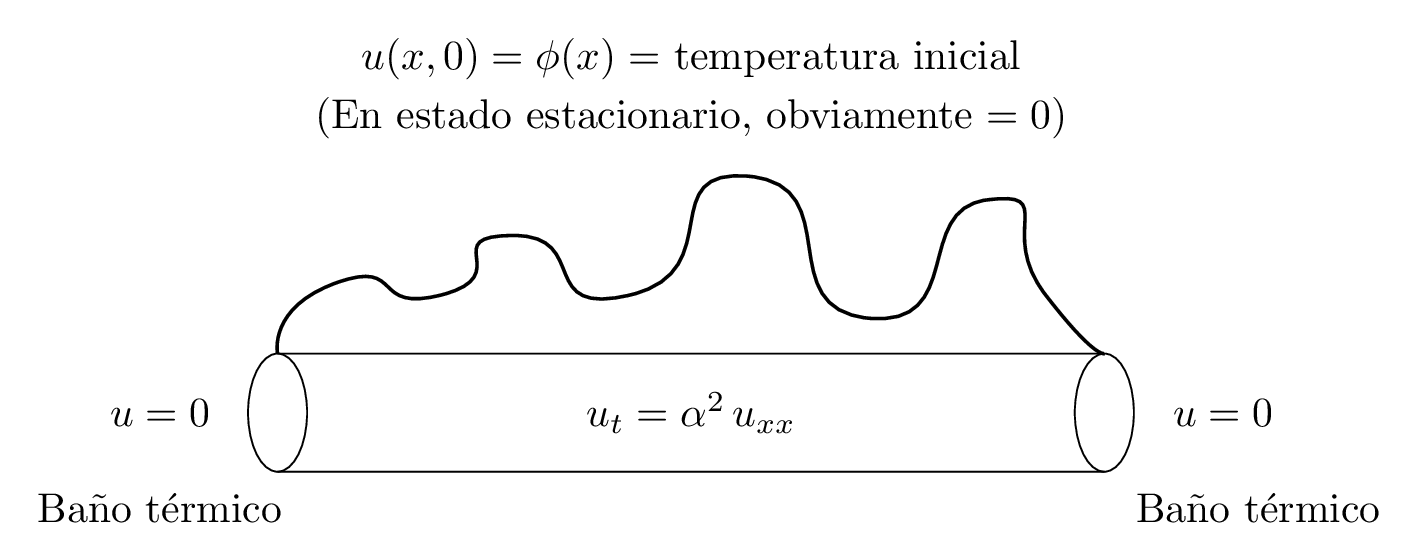
\includegraphics[scale=0.25]{Imagenes/Separacion_Variables_00_Barra.png}
    \caption{Esquema que representa la barra conductora así como las condiciones iniciales y de frontera.}
    \label{fig:figura_barra_01}
\end{figure}

También se nos dan datos sobre el problema en forma de condición inicial; nuestro objetivo es encontrar la temperatura $u (x, t)$ en puntos posteriores en el tiempo.

Ahora veamos una descripción general.

\subsection{La técnica.}

El método de separación de variables supone la existencia de soluciones sencillas de una EDP de la forma:
\begin{align*}
u (x, t) =  X (x) \, T (t)
\end{align*}
donde $X (x)$ es alguna \emph{función que depende solo de} $x$ y $T (t)$ es alguna \emph{función que depende solo de} $t$.
\par
Las soluciones son sencillas porque cualquier temperatura $u (x, t)$ de esta forma conservará su \enquote{forma} básica para diferentes valores de tiempo $t$, como podemos ver en la figura (\ref{fig:figura_separacion_variables_01})
\begin{figure}[H]
    \centering
    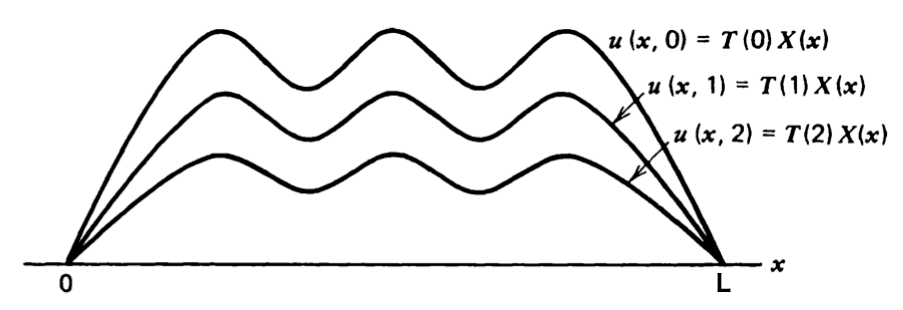
\includegraphics[scale=0.4]{Imagenes/Separacion_Variables_01.png}
    \caption{Gráfica de $X(x)$ y $T(t)$ para distintos valores de $t$.}
    \label{fig:figura_separacion_variables_01}
\end{figure}
La idea general que tenemos nos plantea la posibilidad de encontrar un número infinito de estas soluciones a la EDP (que al mismo tiempo también satisfacen las condiciones de frontera). Estas funciones simples
\begin{align*}
u_{n} (t) = X_{n} (x) \, T_{n} (t)
\end{align*}
se les denomina \textbf{soluciones fundamentales}, son las componentes básicas de nuestro problema, y de la solución $u (x, t)$ que estamos buscando. Sumando las soluciones fundamentales $X_{n} (x) \, T_{n} (t)$ de tal manera que la suma resultante
\begin{align*}
\nsum_{n=1}^{\infty} A_{n} \, X_{n} (x) \, T_{n} (t)
\end{align*}
satisface las condiciones iniciales. Dado que esta suma aún satisface la EDP y las CDF, ahora tenemos la solución a nuestro problema. Veamos a detalle el método de separación de variables.

\subsection{Paso 1. Encontrar las soluciones elementales de la EDP.}

Nos interesa encontrar la función $u (x, t)$ que satisfaga las siguientes condiciones:
\begin{align*}
\text{EDP} \hspace{1.5cm} &u_{t} = \alpha^{2} \, u_{xx} \hspace{1cm} 0 < x < L, \hspace{0.3cm} 0 < t < \infty \\[0.5em] 
\text{CDF} \hspace{1.5cm} &\begin{cases}
u (0, t) = 0 \\
u (L, t) = 0
\end{cases}
\hspace{1cm}
0 < t < \infty \\[0.5em]
\text{CI} \hspace{1.5cm} & u (x, 0) = \phi (x) \hspace{1cm} 0 \leq x \leq L
\end{align*}
Para comenzar, buscamos soluciones de la forma $u (x, t) = X (x) \, T (t)$ sustituyendo $X (x) \, T (t)$ en la EDP y resolvemos para  $X (x) \, T (t)$. Haciendo esta sustitución obtenemos:
\begin{align*}
X (x) \, \pderivada{T} (t) = \alpha^{2} \, \sderivada{X} (x) \, T (t)
\end{align*}
La parte que hace todo el trabajo es la siguiente: si \emph{dividimos} cada lado de esta ecuación por $\alpha^{2} \, X (x) \, T (t)$, tenemos que:
\begin{align*}
\dfrac{\pderivada{T} (t)}{\alpha^{2} \, T (t)} = \dfrac{\sderivada{X} (x)}{X (x)}
\end{align*}
para obtener lo que se conoce como \emph{variables separables}, es decir, la expresión del lado izquierdo de la igualdad depende solo de $t$, mientras que la expresión del lado derecho\footnote{El primado sencillo indica la diferenciación de primer grado con respecto a la variable señalada, mientras que el primado doble, señala la diferenciación de segundo grado con respecto a la variable que se indica.}, depende solo de $x$.
\par
Dado que $x$ y $t$ son independientes entre sí, cada lado debe ser una constante fija (digamos $k$),  por tanto podemos escribir:
\begin{align*}
\dfrac{\pderivada{T}}{\alpha^{2} \, T} = \dfrac{\sderivada{X}}{X} = k
\end{align*}
o de manera equivalente
\begin{align*}
\pderivada{T} - k \, \alpha^{2} \, T &= 0 \\[0.5em]
\sderivada{X} - k \, X &= 0
\end{align*}
Entonces, ahora podemos resolver cada uno de estas dos EDO, para luego multiplicarlas y así obtener una solución a la EDP (toma en cuenta que esencialmente hemos cambiado una EDP de segundo orden a dos EDO)
\par
Sin embargo, ahora hacemos una observación importante, a saber, queremos que la constante de separación $k$ sea negativa (o de lo contrario el factor $T (t)$ no se anula cuando $t \to \infty$). Teniendo esto en cuenta, es una práctica general cambiar el nombre de $k = - \lambda$, donde $\lambda$ es distinta de cero. Llamando a nuestra \emph{constante de separación} por su nuevo nombre, ahora podemos escribir las dos EDO como:
\begin{align*}
\pderivada{T} + \lambda \, \alpha^{2} \, T &= 0 \\[0.5em]
\sderivada{X} + \lambda \, X &= 0
\end{align*}
Ahora podemos resolver ese par de ecuaciones, para $\sderivada{X} + \lambda \, X = 0$ son de la forma:
\begin{align}
\begin{cases}
X (x) = A + B \, x & \hspace{0.2cm} \lambda = 0 \\
X (x) = A \, e^{a x} + B \, e^{-a x} & \hspace{0.2cm} \lambda = - a^{2} \\
X (x) = A \cos (a x ) + B \, \sin (a x) & \hspace{0.2cm} \lambda = a^{2}
\end{cases}
\label{eq:ecuacion_06_02_31}
\end{align}
mientras que para $\pderivada{T} + \lambda \, \alpha^{2} \, T = 0$ se tiene:
\begin{align}
T (t) = A \, e^{- \lambda \, \alpha^{2} \, t} \hspace{1.5cm} \text{con A arbitraria}
\label{eq:ecuacion_06_02_36a}    
\end{align}
y de aquí
\begin{align*}
u (x, t) = X (x) \, T (t) 
\end{align*}
En este punto, tenemos un número infinito de funciones que satisfacen la EDP.

\newpage

\subsection{Paso 2. Encontrar las soluciones de la EDP con las CDF.}

Ahora debemos de considerar un subconjunto de las soluciones obtenidas en el paso anterior, que a su vez satisfagan las condiciones de frontera (CDF):
\begin{align*}
u (0, t) &= 0 \\[0.5em]
u (L, t) &= 0
\end{align*}
por las CDF únicamente en las posibles soluciones para $X (x)$ (ec. \ref{eq:ecuacion_06_02_31}), la tercera posibilidad produce una solución no trivial. De hecho, trabajando con
\begin{align*}
X (x) = A \cos (a x) + B \, \sin (a x) \hspace{2cm}
\end{align*}
que al sustituir en la solución:
\begin{align*}
u (0, t) &= A \, e^{-\lambda \alpha^{2} \, t} = 0 \hspace{0.3cm} \Longrightarrow \hspace{0.3cm} A = 0 \\[0.5em]
u (L, t) &= B \, e^{-\lambda \alpha^{2} \, t} \, \sin (\lambda \, L) = 0 \hspace{0.3cm} \Longrightarrow \hspace{0.3cm} \sin (\lambda \, L) = 0
\end{align*}
Esta última CDF restringe la constante de separación $\lambda$ de ser cualquier número distinto de cero, debe ser una raíz de la ecuación $\sin (\lambda \, L) = 0$. En otras palabras, para que $u (L, t) = 0$, es necesario elegir
\begin{align}
\lambda \, L = n \, \pi \hspace{1.5cm} n \in \mathbb{Z}
\label{eq:ecuacion_06_02_34}    
\end{align}
Sin embargo, para no contar dos veces la misma solución se toma $n$ positivo, es decir:
\begin{align}
\lambda = \dfrac{n^{2} \, \pi^{2}}{L^{2}} \hspace{1.5cm} n = 1, 2, 3, \ldots
\label{eq:ecuacion_06_02_35}
\end{align}
En este paso hemos encontrado un número infinito de funciones que son solución a la EDP:
\begin{align}
u_{n} (x, t) = A_{n} \, \exp \left( - \dfrac{n^{2} \, \alpha^{2} \, \pi^{2}}{L^{2}} \, t \right) \, \sin \left( \dfrac{n \, \pi}{L} \, x \right)
\label{eq:ecuacion_06_02_37}    
\end{align}
por el principio de superposición, la solución que se propone es:
\begin{align}
u (x, t) = \nsum_{n=1}^{\infty} A_{n} \, \exp \left( - \dfrac{n^{2} \, \alpha^{2} \, \pi^{2}}{L^{2}} \, t \right) \, \sin \left( \dfrac{n \, \pi}{L} \, x \right)
\label{eq:ecuacion_06_02_38}
\end{align}
Nos queda por considerar las condiciones iniciales del problema para obtener entonces la solución a la EDP.

\subsection{Paso 3. Encontrar la solución de la EDP, con las CDF y la condición inicial.}

El último paso (y probablemente el más interesante desde un punto de vista matemático) es agregar las soluciones fundamentales (ec. \ref{eq:ecuacion_06_02_38} de tal manera (eligiendo los coeficientes $A_{n}$) que la condición inicial:
\begin{align*}
u (x, 0) = \phi (x)
\end{align*}
se satisfaga. Utilizando la CI en la suma, se tiene que:
\begin{align*}
\phi (x) = \nsum_{n=1}^{\infty} A_{n} \, \sin \left( \dfrac{n \, \pi}{L} \, x \right)
\end{align*}
Vemos que esto es equivalente a encontrar el desarrollo en series\footnote{Se debe de ocupar el desarrollo en una serie de Fourier y ocupar la propiedad de ortogonalidad de la función seno.} de la función seno de $\phi (x)$, que tiene por solución:
\begin{align}
A_{n} = \dfrac{2}{L} \scaleint{6ex}_{\bs 0}^{L} \phi (x) \, \sin \left( \dfrac{n \, \pi}{L} \, x \right) \dd{x}
\label{eq:ecuacion_06_02_40}    
\end{align}
por lo que la solución al problema de Dirichlet para la ecuación de calor es:
\begin{align}
\resizebox{0.9\hsize}{!}{
\addtolength{\fboxsep}{5pt}\boxed{
u (x, t) = \dfrac{2}{L} \nsum_{n=1}^{\infty} \left[ \scaleint{6ex}_{\bs 0}^{L} \phi (x) \, \sin \left( \dfrac{n \pi}{L} x \right) \dd{x} \right] \exp \left( - \dfrac{n^{2} \alpha^{2} \pi^{2}}{L^{2}} t \right) \, \sin \left( \dfrac{n \pi}{L} x \right)
}}
\label{eq:ecuacion_06_02_41}    
\end{align}
Este seguimiento de pasos es el que se debe de utilizar cuando aplicamos el método de separación de variables. Con el ejercicio del caso unidimensional, encontramos una solución a las EDO resultantes, en el siguiente ejercicio veremos un caso con una complejidad mayor, y que nos va a devolver una ecuación diferencial con ciertas características que revisaremos más adelante en el curso.

%Ref. Zamora (2012) - Notas EDP 2.1.6 Lámina rectangular
\section{Ecuación de calor en un lámina rectangular.}

Consideremos ahora el problema de \emph{conducción de calor en dos dimensiones} en un sistema cartesiano:
\begin{align}
u_{t} = \alpha^{2} \, \laplacian{u}
\label{eq:ecuacion_02_187}
\end{align}

Con las condiciones de frontera (CDF):
\begin{align}
u (0, y, t) &= 0 \label{eq:ecuacion_02_188} \\
u (a, y, t) &= 0 \label{eq:ecuacion_02_189} \\
u (x, 0, t) &= 0 \label{eq:ecuacion_02_190} \\
u (x, b, t) &= 0 \label{eq:ecuacion_02_191} \\
0 < t &< \infty \nonumber
\end{align}

Y las condiciones iniciales (CI):
\begin{align}
u (x, y, 0) = f (x, y) \label{eq:ecuacion_02_192}
\end{align}

definido para $0 < x < a$, $0  < y < b$ y $t > 0$.
\begin{figure}[H]
    \centering
    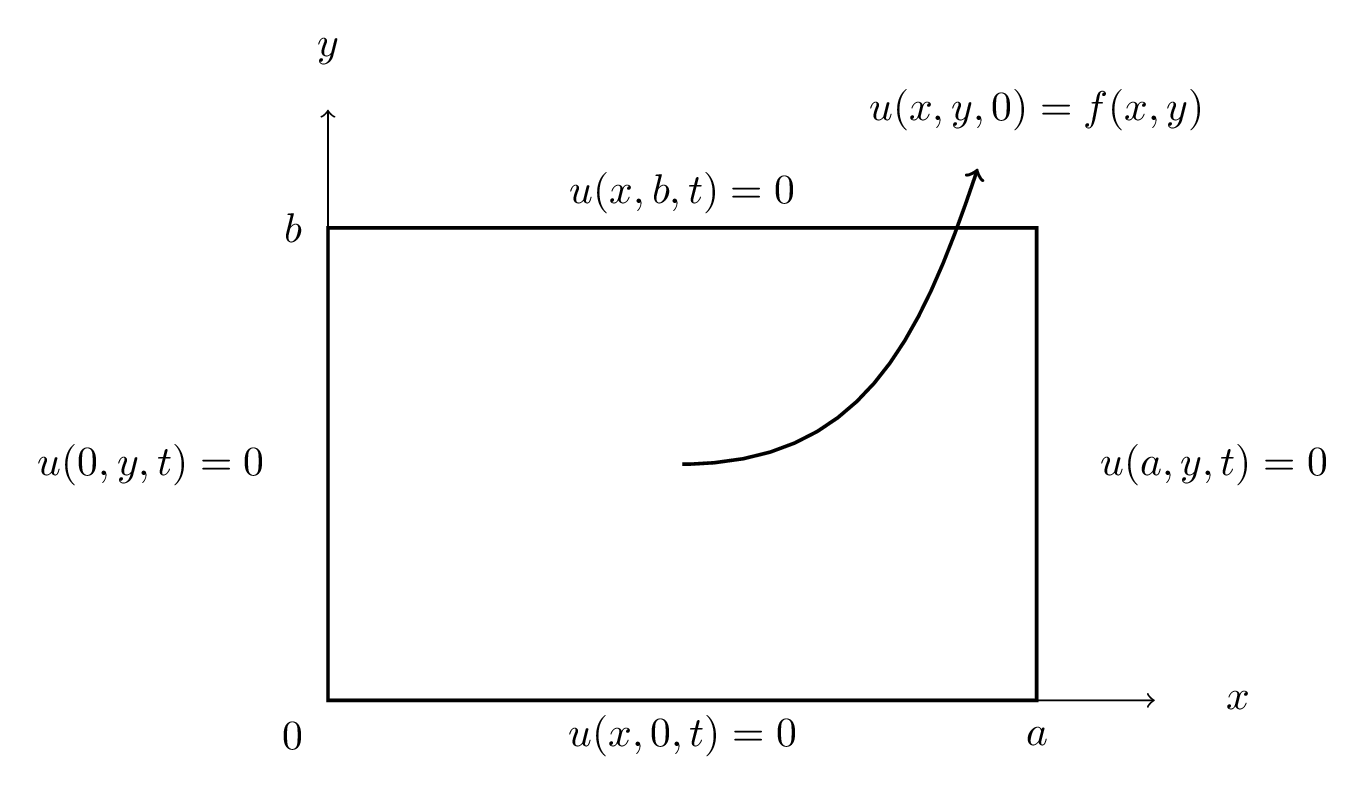
\includegraphics[scale=0.325]{Imagenes/Separacion_Variables_01_Lamina_Cuad.png}
    \caption{Región de una lámina cuadrada para resolver el problema.}
    \label{fig:figura_lamina_cuadrada}
\end{figure}

Ocuparemos la definición del operador de Laplace o Laplaciano en dos dimensiones $x$, $y$:
\begin{align}
\laplacian{u} = u_{xx} + u_{yy}
\label{eq:ecuacion_02_193}
\end{align}
Nótese que, a pesar que $u$ es función tanto de $(x, y) $ como de $t$, el Laplaciano sólo actúa en las coordenadas espaciales.
\par
Podemos interpretar este problema como la difusión de calor a través de la frontera de la lámina rectangular $[0, a] \cp [0, b]$ cuando esta lámina se encuentra aislada térmicamente tanto en su área superior como en su área inferior, como se aprecia en la fig (\ref{fig:figura_lamina_cuadrada}). Las condiciones de frontera (\ref{eq:ecuacion_02_188})-(\ref{eq:ecuacion_02_191}) para este problema especifican una temperatura constante cero en todo el perímetro del rectángulo.
\par
La propuesta de solución para la técnica de separación de variables es para este caso:
\begin{align}
u (x, y, t) = X (x) \, Y (y) \, T (t)
\label{eq:ecuacion_02_194}
\end{align}

Recordemos que cada función con mayúscula depende de una sola variable.
\par
Calculamos las derivadas parciales que habrá que sustituir en la ecuación (\ref{eq:ecuacion_02_194}):
\begin{align*}
u_{t} &= X (x) \, Y (y) \, \pderivada{T} (t) \\[0.5em]
u_{xx} &= \sderivada{X} (x) \, Y (y) \, T (t) \\[0.5em]
u_{yy} &= X (x) \, \sderivada{Y} (y) \, T (t)
\end{align*}
por lo que tendremos:
\begin{align*}
X (x) \, Y (y) \, \pderivada{T} (t) = \alpha^{2} \left[ \sderivada{X} (x) \, Y (y) \, T (t) + X (x) \, \sderivada{Y} (y) \, T (t) \right]
\end{align*}

Continuamos con el siguiente paso: que es dividir entre la solución propuesta.
\par
Ahora dividimos entre $X (x) \, Y (y) \, T (t)$, obteniendo:
\begin{align*}
\dfrac{\pderivada{T} (t)}{\alpha^{2}  \, T (t)} = \left[ \dfrac{\sderivada{X} (x)}{X (x)} + \dfrac{\pderivada{Y} (y)}{Y (y)} \right]
\end{align*}

en donde encontramos que la expresión del lado izquierdo de la igualdad depende solo de la variable $t$, mientras que la expresión del lado derecho depende tanto de $x$ e $y$.
\par
Como $t$, $x$, $y$ son variables independientes, la igualdad solo puede ser posible si ambas funciones son iguales a una función constante.
\begin{align*}
\dfrac{\pderivada{T} (t) }{T (t)} =  \alpha^{2} \left[ \dfrac{\sderivada{X} (x)}{X (x)} + \dfrac{\pderivada{Y} (y)}{Y (y)} \right] = A
\end{align*}

Donde $A$ es una constante por determinar.

Tendremos entonces la primera EDO:
\begin{align}
\pderivada{T} (t) - A \, T (t) = 0
\label{eq:ecuacion_02_195}
\end{align}

Del curso de EDO I, ya tenemos una idea de cómo resolver esta ecuación, quedando pendiente definir primera constante de separación $A$.
\par
Tomando por separado la igualdad del lado derecho, tendremos una segunda constante de separación:
\begin{align*}
\left[ \dfrac{\sderivada{X} (x)}{X (x)} + \dfrac{\pderivada{Y} (y)}{Y (y)} \right]  = \dfrac{A}{\alpha^{2}} = B
\end{align*}    

Avanzando en la revisión del término para las variables $x$ e $y$, se tiene que:
\begin{align*}
\dfrac{\sderivada{X} (x)}{X (x)} = -  \dfrac{\pderivada{Y} (y)}{Y (y)} = C
\end{align*}
y además
\begin{align}
\sderivada{X} (x) - C \, X (x) = 0 \label{eq:ecuacion_02_196} \\[0.5em]
\sderivada{Y} (y) - D \, Y (y) = 0 \label{eq:ecuacion_02_197}
\end{align}
con $A$, $B$, $C$ y $D$ constantes que satisfacen $B = C + D$ y $B = A / \alpha^{2}$, además de las condiciones de frontera:
\begin{align}
X (0) &= 0 \label{eq:ecuacion_02_198} \\[0.5em]
X (a) &= 0 \label{eq:ecuacion_02_199} \\[0.5em]
Y (0) &= 0 \label{eq:ecuacion_02_200} \\[0.5em]
Y (b) &= 0 \label{eq:ecuacion_02_201} \\[0.5em]
\end{align}

Expresando las soluciones para las EDO2H (\ref{eq:ecuacion_02_196}) y (\ref{eq:ecuacion_02_197}) - que son más fáciles de resolver, ya que las derivadas son ordinarias-, se tiene que:
\begin{align}
X (x) &= \sin \left( \dfrac{n \, \pi}{a} \, x \right) \hspace{0.5cm} n = \pm 1, \pm, 2, \ldots \label{eq:ecuacion_02_202} \\[0.5em]
Y (x) &= \sin \left( \dfrac{m \, \pi}{b} \, y \right) \hspace{0.5cm} m = \pm 1, \pm, 2, \ldots \label{eq:ecuacion_02_203}
\end{align}
Por lo que ya es posible determinar las constantes $C$ y $D$:
\begin{align*}
C &= - \dfrac{n^{2} \, \pi^{2}}{a^{2}} \\[0.5em]
D &= - \dfrac{m^{2} \, \pi^{2}}{b^{2}}
\end{align*}
que son constantes negativas.
\par
Notemos el hecho de que $C = 0$ (o $D = 0$) no es posible, ya que la solución sería:
\begin{align*}
X (x) = c_{1} \, x + c_{2} \hspace{1cm} \mbox{o } \hspace{0.3cm} Y (y) = c_{1} \, y + c_{2}
\end{align*}
que nos daría $X (x) \equiv 0$ (o $Y (y) \equiv 0$) al utilizar las condiciones de frontera.
\par
Ahora entonces, ya podemos calcular la constante $B$:
\begin{align*}
B = C + D = - \left( \dfrac{n^{2}}{a^{2}} + \dfrac{m^{2}}{b^{2}} \right) \, \pi^{2}
\end{align*}
y como la constante $B = A / \alpha^{2}$, tenemos que:
\begin{align}
A = - \left( \dfrac{n^{2}}{a^{2}} + \dfrac{m^{2}}{b^{2}} \right) \, \pi^{2} \, \alpha^{2}
\label{eq:ecuacion_02_204}
\end{align}
Con estos resultados, ya podemos presentar la solución de la EDO2H (\ref{eq:ecuacion_02_195}):
\begin{align}
T (t) = \exp\left[ - \left( \dfrac{n^{2}}{a^{2}} + \dfrac{m^{2}}{b^{2}} \right) \, \pi^{2} \, \alpha^{2} \, t \right]
\label{eq:ecuacion_02_205}
\end{align}
Al tener ya una solución para cada una de las EDO2H, presentamos la solución general para nuestro problema:
\begin{align}
u_{nm} (x, y, t) = \sin \left( \dfrac{n \, \pi}{a} \, x \right) \, \sin \left( \dfrac{m \, \pi}{b} \, y \right) \, \exp\left[ - \left( \dfrac{n^{2}}{a^{2}} + \dfrac{m^{2}}{b^{2}} \right) \, \pi^{2} \, \alpha^{2} \, t \right]
\label{eq:ecuacion_02_206}
\end{align}
Tomando la combinación lineal más general (principio de superposición) e intercambiando la suma sobre los enteros negativos por una sobre los positivos, llegamos a:
\begin{align}
&u (x, y, t) = \nsum_{n=1}^{\infty} \nsum_{m=1}^{\infty} b_{mn} \, u_{nm} (x, y, t) = \label{eq:ecuacion_02_207} \\[0.5em]
&= \nsum_{n=1}^{\infty} \nsum_{m=1}^{\infty} b_{mn} \sin \left( \dfrac{n \pi}{a} x \right) \sin \left( \dfrac{m \pi}{b} y \right) \exp\left[ - \left( \dfrac{n^{2}}{a^{2}} {+} \dfrac{m^{2}}{b^{2}} \right) \pi^{2} \alpha^{2} t \right] \label{eq:ecuacion_02_208}
\end{align}

Esta ecuación satisface las CDF e iniciales, pero donde los coeficientes $b_{mn}$ están aún por determinar por la condición inicial (\ref{eq:ecuacion_02_192}). Evaluando ésta en $u (x, y, t)$ en $t = 0$ y con la condición (\ref{eq:ecuacion_02_192}), obtenemos que:
\begin{align}
f (x,y) = \nsum_{p=1}^{\infty} \nsum_{q=1}^{\infty} b_{pq} \sin \left( \dfrac{p \pi}{a} x \right) \sin \left( \dfrac{q \pi}{b} y \right) 
\end{align}
en donde se ha hecho un cambio de índices mudos. Al multiplicar ambos lados por el producto:
\begin{align*}
\sin \left( \dfrac{n \pi}{a} x \right) \sin \left( \dfrac{m \pi}{b} y \right) 
\end{align*}
e integrando sobre el rectángulo $[0, a] \cp [0, b]$, llegamos a:
\begin{align}
\begin{aligned}[b]
\scaleint{6ex}_{\bs 0}^{a} \scaleint{6ex}_{\bs 0}^{b} & f (x, y) \sin \left( \dfrac{n \pi}{a} x \right) \sin \left( \dfrac{m \pi}{b} y \right) \dd{x} \dd{y} = \\[0.5em]
&=\left( \dfrac{a b}{4} \right) \nsum_{p=1}^{\infty} \nsum_{q=1}^{\infty} b_{pq} \delta_{pn} \delta_{qm}
\end{aligned}
\label{eq:ecuacion_02_210}
\end{align}
en donde se ha utilizado:
\begin{align}
\scaleint{6ex}_{\bs 0}^{a} \sin \left( \dfrac{p \pi}{a} x \right) \sin \left( \dfrac{n \pi}{a} x \right) \dd{x} &= \dfrac{a}{2} \, \delta_{pn} \label{eq:ecuacion_02_211} \\[0.5em]
\scaleint{6ex}_{\bs 0}^{b} \sin \left( \dfrac{q \pi}{b} y \right) \sin \left( \dfrac{m \pi}{b} y \right) \dd{y} &= \dfrac{b}{2} \, \delta_{qm} \label{eq:ecuacion_02_212}
\end{align}
Llevando a cabo las sumas en la ec. (\ref{eq:ecuacion_02_210}), llegamos al resultado que determina los coeficientes $b_{nm}$:
\begin{align}
b_{mn} = \dfrac{4}{ab} \scaleint{6ex}_{\bs 0}^{a} \scaleint{6ex}_{\bs 0}^{b} f (x, y) \sin \left( \dfrac{n \pi}{a} x \right) \sin \left( \dfrac{m \pi}{b} y \right) \dd{x} \dd{y}
\label{eq:ecuacion_02_213}
\end{align}
De esta manera la solución completa para este problema de una lámina rectangular, está dada por la función $u (x, y, t)$ de la ec. (\ref{eq:ecuacion_02_208}), con los coeficientes $b_{mn}$ dados por la ec. (\ref{eq:ecuacion_02_213}), que es válida para toda $(x, y) \in [0, a] \cp [0, b]$ y para todo $t \geq 0$. 

%Referencia. Arfken (2006) - 9.3 Separation of variables

\section{Coordenadas cilíndricas \texorpdfstring{$(\rho, \varphi, z)$}{(r, v, z)}.}

En el siguiente ejercicio ocuparemos nuevamente el método de separación de variables, en donde no se han especificado las condiciones de frontera ni las condiciones iniciales; la geometría en donde se plantea el problema es con el sistema coordenado cilíndrico, y como partimos de una ecuación que involucra al operador diferencial Laplaciano, se debe de representar en la respectiva geometría, el correspondiente Laplaciano. Este ejercicio sirve de base para demostrar que una ecuación diferencial es separable en otra simetría.

\subsection{Ecuación de Helmholtz.}

Consideremos una función desconocida $\psi$ que depende de $\rho, \varphi$ y $z$, la ecuación de Helmholtz se expresa como:
\begin{align}
\laplacian{\psi (\rho, \varphi, z)} + k^{2} \, \psi (\rho, \varphi, z) = 0
\label{eq:ecuacion_09_45}    
\end{align}

\subsection{Ecuación en coordenadas cilíndricas.}

En coordenadas cilíndricas\footnote{Aquí recuperamos lo que vimos en el Tema 1 - La física y la geometría, ya que para expresar el operador laplaciano, debemos de ocupar los factores de escala para este sistema coordenado.} la ecuación de Helmholtz tiene la forma:
\begin{align}
\dfrac{1}{\rho} \, \pdv{\rho} \left( \rho \, \pdv{\psi}{\rho} \right) + \dfrac{1}{\rho^{2}} \, \pdv[2]{\psi}{\varphi} + \pdv[2]{\psi}{z} + k^{2} \, \psi = 0
\label{eq:ecuacion_09_46}
\end{align}
Ocuparemos la primera suposición que vimos en el ejemplo anterior para la ecuación de calor, es decir, suponemos que existe una solución del tipo
\begin{align}
\psi (\rho, \varphi, z) = P (\rho) \, \Phi (\varphi) \, Z (z)
\label{eq:ecuacion_09_47}
\end{align}
Sustituyendo en la ecuación (\ref{eq:ecuacion_09_46}), tendremos que\footnote{Como se ha definido que las funciones $P$, $\Phi$ y $Z$ dependen cada una de ellas de una sola variable, podemos ahorrar en la escritura la dependencia de esa variable, quedando la expresión más clara y entendible.}:
\begin{align}
\dfrac{\Phi \, Z}{\rho} \, \dv{\rho} \left( \rho \, \dv{P}{\rho} \right) + \dfrac{\Phi \, Z}{\rho^{2}} \, \dv[2]{\Phi}{\varphi} + P \, \Phi \, \dv[2]{Z}{z} + k^{2} \, P \, \Phi \, Z = 0 
\label{eq:ecuacion_09_48}    
\end{align}
Todas las derivadas parciales quedan como derivadas ordinarias, ya que las funciones dependen sólo de una variable. Dividiendo entre $P \, \Phi \, Z$, dejando el término de la derivada de $z$ a la derecha de la igualdad, resulta en:
\begin{align}
\dfrac{1}{\rho \, P} \dv{\rho} \left( \rho \, \dv{P}{\rho} \right) + \dfrac{1}{\rho^{2} \, \Phi} \, \dv[2]{\Phi}{\varphi} + k^{2} =  - \dfrac{1}{Z} \, \dv[2]{Z}{z}
\label{eq:eq:ecuacion_09_49}
\end{align}
Encontramos que una función de $z$ a la derecha parece depender de una función de $\rho$ y $\varphi$ a la izquierda. Resolvemos esto haciendo que cada lado de la ec. (\ref{eq:eq:ecuacion_09_49}) sea igual a la misma constante.

\subsection{Primera constante de separación.}

La elección del signo de la constante de separación es arbitraria. Sin embargo, se elige un signo menos para la coordenada axial $z$ con la expectativa de una posible dependencia exponencial de $z$ (de la ec. (\ref{eq:ecuacion_09_50})). Se elige un signo positivo para la coordenada azimutal $\varphi$ con la expectativa de una dependencia periódica de $\varphi$ (de la ec. (\ref{eq:ecuacion_09_53})).
\par
Escogemos la constante de separación $- l^{2}$. Por tanto, tenemos el sistema:
\begin{align}
\dv[2]{Z}{z} &= l^{2} \, Z \label{eq:ecuacion_09_50} \\[0.5em]
\dfrac{1}{\rho \, P} \dv{\rho} \left( \rho \, \dv{P}{\rho} \right) + \dfrac{1}{\rho^{2} \, \Phi} \dv[2]{\Phi}{\varphi} + k^{2} &= - l^{2} \label{eq:ecuacion_09_51}
\end{align}
Haciendo $k^{2} + l^{2} = n^{2}$, multiplicando por $\rho^{2}$, y reordenando los términos tenemos:
\begin{align}
\dfrac{\rho}{P} \dv{\rho} \left( \rho \, \dv{P}{\rho} \right) + n^{2} \, \rho^{2} = - \dfrac{1}{\Phi} \, \dv[2]{\Phi}{\varphi}
\label{eq:ecuacion_09_52}
\end{align}

\subsection{Segunda constante de separación.}

Si definimos que la expresión del lado derecho sea igual a $m^{2}$, que en este caso representa la segunda constante de separación, entonces:
\begin{align}
\dv[2]{\Phi}{\varphi} = - m^{2} \, \Phi
\label{eq:ecuacion_09_53}
\end{align}
Para el término con dependencia en $\rho$, se tiene
\begin{align}
\rho \, \dv{\rho} \left( \rho \, \dv{P}{\rho} \right) + (n^{2} \, \rho^{2} - m^{2}) \, P = 0
\label{eq:ecuacion_09_54}
\end{align}
Esta última ecuación se le conoce como la \textbf{ecuación diferencial de Bessel}, cuya solución y sus propiedades se presentarán en el Tema 4 - Funciones Especiales. 
\par
Como dato adicional: la separación de variables de la ecuación de Laplace en coordenadas parabólicas también devuelve la ecuación de Bessel, es decir, bajo una geometría en particular, se obtendrán ecuaciones diferenciales con relevancia para la física matemática.
\par
La ecuación de Helmholtz inicial (ec. \ref{eq:ecuacion_09_45}), que es una EDP en tres dimensiones y ocupando dos constantes de separación \iffalse \footnote{Como vemos, si $n$ es el orden de la EDP, entonces tendremos $n-1$ constantes de separación.} \fi, ha sido reemplazada por tres EDO (\ref{eq:ecuacion_09_50}), (\ref{eq:ecuacion_09_53}) y (\ref{eq:ecuacion_09_54}). Una solución de la ecuación de Helmholtz es:
\begin{align}
\psi (\rho, \varphi, z) = P(\rho) \, \Phi (\varphi) \, Z(z)
\label{eq:ecuacion_09_55}    
\end{align}

\subsection{Solución general.}

Identificando las soluciones específicas para $P, \Phi, Z$ por los subíndices, la solución más general de la ecuación de Helmholtz, es una combinación lineal del producto de las soluciones:
\begin{align}
\Psi (\rho, \varphi, z) =  \nsum_{m,n} a_{mn} \, P_{mn}(\rho) \, \Phi_{m}(\varphi) \, Z_{n}(z)
\label{eq:ecuacion_09_56}
\end{align}
Para resolver un caso particular, se deberán de tener en cuenta las condiciones de frontera, así como las condiciones iniciales, que nos devolvería una solución particular a un problema.
\chapter{Método de Frobenius.}

\section{Método de Frobenius.}
\subsection{Introducción.}
%Ref. Bruzzone - Introducción al método de Frobenius

El método propone la búsqueda de soluciones en series de potencias para ecuaciones diferenciales lineales de segundo orden.
\par
Este procedimiento requiere el encontrar relaciones de recurrencia entre los coeficientes de las series buscadas, asumiendo que el primer término de la serie es no nulo.

\subsection{Soluciones analíticas.}

Una clase muy extensa de ecuaciones diferenciales poseen soluciones que se expresan en series de potencias, las cuales son válidas en un dominio determinado. Las funciones que gozan de esta particularidad se les llama \emph{analíticas}.
\par
Las ecuaciones diferenciales más familiares como la ecuación de un oscilador armónico:
\begin{align*}
\ddot{x} + \omega^{2} \, x = 0
 \end{align*}
admite soluciones del tipo
\begin{align*}
x(s) = A_{1} \, \sin(\omega \, s) + A_{2} \, \cos (\omega \, s)
\end{align*}
siendo claro que $\sin(\omega \, s)$ y $\cos(\omega \, s)$ son funciones analíticas.
\par
De igual manera para la ecuación de un oscilador amortiguado, como en un gran número de ecuaciones de la mecánica nos encontraremos que forman parte de este tipo de ecuaciones.

\subsection{Definición.}

Una expresión de la forma:
\begin{align}
a_{0} + a_{1} \, (x - x_{0}) + \ldots + a_{n} \, x^{n} = \nsum_{n=0}^{\infty} a_{n} \, (x - x_{0})^{n}
\label{eq:ecuacion_01}    
\end{align}
se llama \textit{serie de potencias}.
\par
La serie puede estar definida por el límite
\begin{align*}
\lim_{N \to \infty} \nsum_{n=0}^{N} a_{n} \, (x - x_{0})
\end{align*}
para aquellos valores de $x$ en que exista el límite. En ese caso, se le conoce a la serie como una serie convergente.
\par
Para determinar los valores de $x$ que cumplen la condición de convergencia, se utiliza el criterio del cociente:
\begin{align*}
\lim_{n \to \infty} \dfrac{a_{n+1}}{a_{n}} = \rho \hspace{1.5cm} \begin{cases}
\text{Converge si } & \rho < 1 \\
\text{Diverge si } & \rho > 1
\end{cases}
\end{align*}
El criterio no clasifica si $\rho = 1$.
\par
Más general es considerar el valor absoluto de dicho cociente, si está acotado por cierto numero $\sigma$ cuando $n \to \infty$, la serie converge cuando $\sigma < 1$. Por lo tanto, tendríamos que
\begin{align*}
\rho = \lim_{n \to \infty} \abs{\dfrac{a_{n+1}}{a_{n}}} \, \abs{x - x_{0}} = L \, \abs{x - x_{0}}
\end{align*}
en donde
\begin{align*}
L = \lim_{n \to \infty} \abs{\dfrac{a_{n+1}}{a_{n}}}
\end{align*}
\par
Si este límite existe, se deduce por la ec. (\ref{eq:ecuacion_01}):
\begin{align}
\begin{aligned}        
\text{converge si } &\abs{x - x_{0}} < \dfrac{1}{L} \\[0.5em]
\text{diverge si } &\abs{x - x_{0}} > \dfrac{1}{L}
\end{aligned}
\label{eq:ecuacion_02}    
\end{align}
De esta manera tendremos un intervalo de convergencia cuando $L$ existe:
\begin{align*}
\bigg( x_{0} - \dfrac{1}{L}, x_{0} + \dfrac{1}{L} \bigg)
\end{align*}
Este intervalo es simétrico respecto de $x_{0}$, de manera tal que \textbf{la serie es convergente dentro} de este intervalo y \textbf{divergente fuera} del mismo.

\section{Puntos singulares.}
\subsection{Definiciones.}
%Ref. Arfken

Se presenta el concepto de un \textbf{punto singular o singularidad} (tal como se aplica a una ecuación diferencial).
\par
El interés en este concepto radica en su utilidad en:
\begin{enumerate}
\item Clasificar las EDO.
\item Revisar la viabilidad de una solución en series, esta viabilidad es parte del teorema de Fuchs.
\end{enumerate}
Usando la notación $\displaystyle \dv[2]{y}{x} = \sderivada{y}$, tenemos:
\begin{align}
\sderivada{y} = f (x, y, \pderivada{y})
\label{eq:ecuacion_09_74}
\end{align}
Ahora bien, si en la ec. (\ref{eq:ecuacion_09_74}) $y$ e $\pderivada{y}$ pueden tener todos los valores finitos a $x = x_{0}$ e $\sderivada{y}$ permanece finita, el punto $x = x_{0}$ es un \textbf{punto ordinario}.
\par
Por otra parte, si $\sderivada{y}$ se vuelve infinita para cualquier selección finita de $y$ e  $\sderivada{y}$, el punto $x = x_{0}$ se denomina \textbf{punto singular}.
\par
Si escribimos esta EDO2H (en $y$) como
\begin{align}
\sderivada{y} + P (x) \, \tilde{y} + Q(x) \, y = 0
\label{eq:ecuacion_09_75}
\end{align}
Ahora bien, si las funciones $P (x)$ y $Q (x)$ permanecen finitas a $x = x_{0}$, el punto $x = x_{0}$ es un \emph{punto ordinario}.
\par
Al contrario, si $P (x)$ y/o $Q (x)$ divergen mientras $x \to x_{0}$, el punto $x_{0}$ es un \emph{punto singular}.
\par
Usando la ecuación (\ref{eq:ecuacion_09_75}) podemos distinguir entre dos tipos de puntos singulares:
\begin{enumerate}
\item Si $P (x)$ y/o $ Q(x)$ divergen a medida que $x \to x_{0}$, pero $(x - x_{0}) \: P (x)$ y $(x - x_{0})^{2} \: Q (x)$ permanecen finitas a medida que $x \to x_{0}$, entonces el punto $x = x_{0}$ se llama \textbf{punto singular regular o punto singular no esencial}.
\item Si $P (x)$ diverge más rápidamente que $\dfrac{1}{(x - x_{0})}$, de tal modo que $(x - x_{0}) \: P (x)$ tiene a infinito a medida que $x \to x_{0}$, o cuando $Q (x)$ diverge más rápidamente que $\dfrac{1}{(x - x_{0})^{2}}$, de modo que $(x - x_{0})^{2} \: Q (x)$ tiene a infinito, a medida que $x \to x_{0}$, entonces el punto $x = x_{0}$ se llama \textbf{singularidad esencial o singularidad irregular}.
\end{enumerate}
Estas definiciones son válidas para todos los valores finitos de $x_{0}$. 
\par
El análisis de los puntos al infinito $(x \to \infty)$ es similar al tratamiento que se hace para las funciones en variable compleja: hacemos el cambio de variable $x = 1/z$, sustituyendo en la ED y entonces hacemos que $z \to 0$. 
\par
Haciendo el cambio de variable en las derivadas:
\begin{align}
\dv{y(x)}{x} = \dv{y(z^{-1})}{z} \: \dv{z}{x} = - \dfrac{1}{x^{2}} \dv{y(z^{-1})}{z} = -z^{2} \: \dv{y(z^{-1})}{z}
\label{eq:ecuacion_09_76}
\end{align}
Entonces:
\begin{align}
\begin{aligned}
\dv[2]{y(x)}{x} &= \dv{z} \left[ \dv{y(x)}{x} \right] \dv{z}{x} = \\
&= (-z^{2}) \left[ -2 \: z \dv{y(z^{-1})}{z} - z^{2} \: \dv[2]{y(z^{-1})}{z} \right] = \\
&= 2 \: z^{3} \: \dv{y(z^{-1})}{z} + z^{4} \: \dv[2]{y(z^{-1})}{z}
\end{aligned}
\label{eq:ecuacion_09_77}
\end{align}
Usando estos resultados, podemos transformar la ecuación (\ref{eq:ecuacion_09_75}) en:
\begin{align}
z^{4} \: \dv[2]{y}{z} + [ 2 \: z^{3} - z^{2} \: P(z^{-1})] \: \dv{y}{z} + Q(z^{-1}) \: y = 0
\label{eq:ecuacion_09_78}
\end{align}
El comportamiento en $x = \infty, (z = 0)$ entonces dependerá del comportamiento de los nuevos coeficientes
\begin{align*}
\dfrac{2 \: z - P(z^{-1})}{z^{2}} \hspace{1cm} \text{ y } \hspace{1cm} \dfrac{Q(z^{-1})}{z^{4}}
\end{align*}
a medida que $z \to 0$.
\par
Si estas dos expresiones se mantienen finitas, el punto $x = \infty$ es un punto ordinario.
\par
Si las expresiones divergen con mayor rapidez que $1/z$ y $1/z^{2}$, respectivamente, el punto $x = \infty$ es un punto regular singular, de otra manera, el punto es irregular singular (una singularidad esencial).

% %Ref. Hassani 2009 Chap. 26
\section{Método de Frobenius.}
\subsection{El método.}

El supuesto básico del método de Frobenius es que la solución de la ED se puede \textbf{representar mediante una serie de potencias}.
\par
Esta no es una suposición restrictiva porque todas las funciones encontradas en aplicaciones físicas pueden escribirse como series de potencias siempre que estemos interesados en sus valores que se encuentran en su intervalo de convergencia.
\par
Este intervalo puede ser muy pequeño o puede cubrir toda la línea real.
\par
Una ecuación diferencial de segundo orden homogénea y lineal, se puede escribir como
\begin{align}
p_{2} (x) \, \dv[2]{y}{x} + p_{1} (x) \, \dv{y}{x} + p_{0} (x) \, y = 0
\label{eq:ecuacion_26_07}    
\end{align}
Para casi todas las aplicaciones que se encuentran en física, consideramos que $p_{0}, p_{1}, p_{2}$ son polinomios.
\par
Es posible que la ED no se presenta en la forma que se muestra a partir de, digamos, el método de separación de variables, pero se puede \enquote{llevar} a esa forma.
\par
La forma más complicada de los coeficientes de las derivadas en una ED son típicamente funciones racionales (razones de dos polinomios).
\par
Por lo tanto, multiplicar la ED por el producto de los tres denominadores nos devolverá la ED en la forma dada en la ec. (\ref{eq:ecuacion_26_07}).
\par
El primer paso en el método de Frobenius es \textbf{asumir una serie de potencias infinita para y}. Es común elegir que el punto de expansión sea $x = 0$.
\par
Si $p_{2} (0) \neq 0$, solo es necesario considerar las potencias no negativas de $x$.
\par
Si $p_{2} (0) = 0$, la ED pierde su carácter de \enquote{segundo orden}, y las soluciones no se revisarían en estas notas.
\par
Se tienen dos opciones:
\begin{enumerate}
\item Elegir un punto de expansión diferente a $x_{0} \neq 0$, tal que $p_{2} (x_{0}) \neq 0$.
\item Permitir las potencias no positivas de $x$ en la expansión de $y$.
\end{enumerate}
Rara vez se utiliza la primera opción. Resulta que la forma más económica, pero general, de incorporar la segunda opción es escribir la solución como se muestra a continuación:
\par
La solución que suponemos es del tipo:
\begin{align}
\begin{aligned}[b]
y &= x^{r} \, \nsum_{n=0}^{\infty} a_{n} \, x^{n} = \\[0.5em]
&= \nsum_{n=0}^{\infty} a_{n} \, x^{n+r} = \\[0.5em]
&= a_{0} \, x^{r} + a_{1} \, x^{r+1} + a_{2} \, x^{r+2} + \ldots
\end{aligned}
\label{eq:ecuacion_26_08}    
\end{align}
donde $r$ es un número real (no necesariamente un entero positivo) que quedará determinado por la ED.
\par
Es habitual elegir $a_{0} = 1$ porque cualquier múltiplo constante de una solución también es una solución.
\par
Si $a_{0} \neq 1$, entonces se multiplica la serie por $1/a_{0}$ y así obtener el valor.
\par
Ya que una serie de potencias es uniformemente convergente (con su radio de convergencia), por lo que se puede diferenciar término a término.
\par
Por lo que al diferenciar la solución en una primera ocasión, tenemos:
\begin{align}
\begin{aligned}[b]
\dv{y}{x} &= \nsum_{n=0}^{\infty} a_{n} \, (n + r) \, x^{n+r-1} = \\[0.5em]
&= r \, a_{0} \, x^{r-1} + (r + 1) \, a_{1} \, x^{r} + \ldots
\end{aligned}
\label{eq:ecuacion_26_09a}
\end{align}
Por lo que al diferenciar por segunda vez, tenemos:
\begin{align}
\begin{aligned}[b]
\dv[2]{y}{x} &= \nsum_{n=0}^{\infty} a_{n} \, (n + r) \, (n + r - 1) \, x^{n+r-1} = \\[0.5em]
&= r \, (r - 1) \, a_{0} \, x^{r-2} + (r + 1) \, r \, a_{1} \, x^{r}-1 + \ldots
\end{aligned}
\label{eq:ecuacion_26_09b}
\end{align}

Ahora sustituimos las ecuaciones (\ref{eq:ecuacion_26_08}), (\ref{eq:ecuacion_26_09a}) y (\ref{eq:ecuacion_26_09b}) en la EDO2H (\ref{eq:ecuacion_26_07}).
\par
Multiplicamos los polinomios en la serie, agrupamos todas las potencias distintas de $x$ y establecemos el coeficiente de cada término igual a cero. Así obtenemos un conjunto de ecuaciones cuya solución determina el valor de $r$ y las $a_{n}$.
\par
La ecuación que surge de la \textbf{potencia más baja de x} involucra solo a $r$, se llama \textbf{ecuación de índices}\footnote{En algunos textos se le conoce como \textbf{ecuación indicial}, que sería una traducción literal del inglés; en estas notas preferimos la referencia como ecuación de índices, ya que es más directa la asociación.}.
\par
Esta suele ser una ecuación cuadrática en $r$ que se puede resolver para obtener el(los) posible(s) valor(es) de $r$, cada uno de los cuales conduce generalmente a una solución diferente.
\par
Las otras ecuaciones que provienen de potencias superiores de $x$ permiten establecer \textbf{relaciones de recurrencia}, es decir, ecuaciones que dan $a_{n}$ en términos de $a_{n-1}$ y $a_{n-2}$. Al iterar esta relación, se pueden obtener todos los $a_{n}$ en términos de solo dos coeficientes.

\subsection{Ejercicio}
% %Ref. Zill ED pág. 279

Resuelve la siguiente EDO2H mediante el método de Frobenius:
\begin{align}
3 \, x \, \sderivada{y} + \pderivada{y} - y = 0
\label{eq:ecuacion_04}    
\end{align}
Como primer paso, proponemos una solución del tipo:
\begin{align*}
y = \nsum_{n=0}^{\infty} a_{n} \, x^{n+r}
\end{align*}
Procedemos a calcular la primera y segunda derivada de la solución:
\begin{align*}
\pderivada{y} &= \nsum_{n=0}^{\infty} (n + r) \, a_{n} \, x^{n+r-1} \\[0.5em]
\sderivada{y} &= \nsum_{n=0}^{\infty} (n + r) \, (n + r - 1) \, a_{n} \, x^{n+r-2}
\end{align*}
Ahora se sustituyen las expresiones en la ED inicial (\ref{eq:ecuacion_04}), de donde obtenemos\footnote{Revisa con cuidado los cambios de signo, ya que en correspondencia con el álgebra, al final del renglón se deja el signo $(+)$, y si el término está restando, en el siguiente renglón se presenta el signo $(-)$.}:
\begin{align*}
3 \, x \, \sderivada{y} + \pderivada{y} - y &= 3 \, x \, \left[  \nsum_{n=0}^{\infty} (n + r) \, (n + r - 1) \, a_{n} \, x^{n+r-2} \right] + \\[0.5em]
&+ \nsum_{n=0}^{\infty} (n + r) \, a_{n} \, x^{n+r-1} - \nsum_{n=0}^{\infty} a_{n} \, x^{n+r} = 0
\end{align*}
Comenzamos a simplificar la expresión:
\begin{align*}
3 \, \left[ \nsum_{n=0}^{\infty} (n + r) \, (n + r - 1) \, a_{n} \, x^{n+r-1} \right] &+ \nsum_{n=0}^{\infty} (n + r) \, a_{n} \, x^{n+r-1} + \\[0.5em]
&- \nsum_{n=0}^{\infty} a_{n} \, x^{n+r} = 0
\end{align*}
Factorizando las primeras sumas:
\begin{align*}
\nsum_{n=0}^{\infty} (n + r) \, \left[ 3 \, (n + r - 1) + 1 \right] \, a_{n} \, x^{n+r-1} - \nsum_{n=0}^{\infty} a_{n} \, x^{n+r} &= 0 \\[0.5em] 
\Rightarrow \hspace{0.3cm} \nsum_{n=0}^{\infty} (n + r) \, (3 \, n + 3 \, r - 2) \, a_{n} \, x^{n+r-1} - \nsum_{n=0}^{\infty} a_{n} \, x^{n+r} &= 0
\end{align*}
La primera suma tiene el exponente más bajo para $x$, extraemos el primer término con $n = 0$, así llegamos a:
\begin{align*}
r (3 \, r - 2) \, a_{0} \, x^{r-1} + \nsum_{n=1}^{\infty} (n + r) \, (3 \, n + 3 \, r - 2) \, a_{n} \, x^{n+r-1} - \nsum_{n=0}^{\infty} a_{n} \, x^{n+r} &= 0
\end{align*}
Sabemos que para factorizar nuevamente las dos sumas, los índices de las mismas deben de comenzar con el mismo valor, así como los exponentes de $x$ deben de ser iguales. Ocupamos la propiedad que tienen los índices en las sumas infinitas: pasamos el índice de $n = 1$ a $n = 0$, haciendo el correspondiente ajuste en los términos que involucran a $n$:
\begin{align*}
r(3 \, r - 2) \, a_{0} \, x^{r-1} &+ \nsum_{n=0}^{\infty} (n + r + 1) \, (3 \, (n + 1) + 3 \, r - 2) \, a_{n+1} \, x^{n+r} + \\[0.5em]
&- \nsum_{n=0}^{\infty} a_{n} \, x^{n+r} = 0
\end{align*}    
Al contar ya con los índices que inician en el mismo valor y los exponentes de $x$ son iguales, ya es posible factorizar:
\begin{align*}
r(3 \, r - 2) \, a_{0} \, x^{r-1} &+ \nsum_{n=0}^{\infty} \bigg[ (n + r + 1) \, (3 \, n + 3 \, r + 1) \, a_{n+1} - a_{n} \bigg] \, x^{n+r} = 0    
\end{align*}
De la teoría de series infinitas, sabemos que todos los coeficientes de la suma deben de ser nulos, y como $a_{0} \neq 0$ desde la propuesta de la solución en series: tenemos dos resultados importantes, el primero de ellos lo consideramos de la expresión con el exponente más pequeño del desarrollo:
\begin{align*}
r \, (3 \, r - 2) \, a_{0} = 0
\end{align*}
que es la \textbf{ecuación de índices}.
\par
El segundo resultado es la \textbf{relación de recurrencia}:
\begin{align*}
(n + r + 1)(3 \, n + 3 \, r + 1) \, a_{n+1} - a_{n} = 0
\end{align*}
Por lo que:
\begin{align}
a_{n+1} = \dfrac{a_{n}}{(n + r + 1)(3 \, n + 3 \, r + 1)}
\label{eq:ecuacion_07}
\end{align}
De la ecuación de índices, sabemos desde el inicio que $a_{0} \neq 0$, por lo que
\begin{align}
r (3 \, r - 2) = 0
\label{eq:ecuacion_06}
\end{align}
que tiene por raíces los valores:
\begin{align*}
r_{1} = \dfrac{2}{3} \hspace{1.5cm} r_{2} = 0
\end{align*}
Ocupamos la primera raíz $r_{1} = 2/3$ en la relación de recurrencia (\ref{eq:ecuacion_07}):
\begin{align}
\begin{aligned}[b]
a_{n+1} &= \dfrac{a_{n}}{ \left( n + \dfrac{2}{3} + 1\right) \left(3 \, n + 3 \, \left( \dfrac{2}{3} \right) + 1\right)} \\[0.5em]
&= \dfrac{a_{n}}{\left( \dfrac{3 \, n + 5}{3} \right) \bigg( 3 (n + 1) \bigg)} = \\[0.5em]
a_{n+1} &= \dfrac{a_{n}}{(3 \, n + 5)(n + 1)} \hspace{1.5cm} n = 0, 1, 2, \ldots
\end{aligned}
\label{eq:ecuacion_08}    
\end{align}
De tal manera que ya podemos calcular los valores de los coeficientes a partir de la relación de recurrencia anterior, ocupando los valores de $n$:
\begin{align*}
a_{1} &= \dfrac{a_{0}}{5 \cdot 1} \\[0.5em]
a_{2} &= \dfrac{a_{1}}{8 \cdot 2} = \dfrac{a_{0}}{2! \, 5 \cdot 8} \\[0.5em]
a_{3} &= \dfrac{a_{2}}{11 \cdot 3} = \dfrac{a_{0}}{3! \, 5 \cdot 8 \cdot 11} \\
\vdots \\[0.5em]
a_{n} &= \dfrac{a_{0}}{n! \, 5 \cdot 8 \cdot 11 \ldots (3\, n + 2)} \hspace{1cm} n = 1, 2, 3, \ldots
\end{align*}
Con este desarrollo hemos obtenido la primera solución $y_{1}(x)$ de la EDO2H inicial, ocupando la raíz $r_{1}$:
\begin{align}
y_{1} (x)= a_{0} \, x^{2/3} \left[ 1 + \nsum_{n=1}^{\infty} \dfrac{a_{0}}{n! \, 5 \cdot 8 \cdot 11 \ldots (3\, n + 2)} \, x^{n} \right]
\label{eq:ecuacion_10}    
\end{align}
Con la segunda raíz de la ecuación de índices: $r_{2} = 0$ se genera una regla de recurrencia distinta:
\begin{align}
a_{n+1} = \dfrac{a_{n}}{(n+1)(3 \, n + 1)} \hspace{1.5cm} n = 0, 1, 2, \ldots
\label{eq:ecuacion_09}    
\end{align}
Por lo que los coeficientes que se obtienen son:
\begin{align*}
a_{1} &= \dfrac{a_{0}}{1 \cdot 1} \\[0.5em]
a_{2} &= \dfrac{a_{1}}{2 \cdot 4} = \dfrac{a_{0}}{2! \, 1 \cdot 4}  \\[0.5em]
a_{3} &= \dfrac{a_{2}}{3 \cdot 7} = \dfrac{a_{0}}{3! \, 4 \cdot 7}  \\[0.5em]
\vdots \\
a_{n} &= \dfrac{a_{0}}{n! \, 1 \cdot 4 \cdot 7 \ldots (3 \, n - 2)} \hspace{1cm} n = 1, 2, 3, \ldots
\end{align*}
La segunda solución $y_{2}(x)$ para la EDO2H inicial es:
\begin{align}
y_{2} (x)= a_{0} \, x^{0} \left[ 1 + \nsum_{n=1}^{\infty} \dfrac{1}{n! \, 1 \cdot 4 \cdot 7 \ldots (3\, n - 2)} \, x^{n} \right]
\label{eq:ecuacion_11}
\end{align}    
Se puede demostrar que las soluciones (\ref{eq:ecuacion_10}) y (\ref{eq:ecuacion_11}) convergen ambas para todos los valores finitos de $x$.
\par
También es posible ver que las soluciones no es múltiplo de la otra, por lo que $y_{1}(x)$ y $y_{2}(x)$ son linealmente independientes con respecto a $x$.
\par
Por el principio de superposición, tenemos que:
\begin{align*}
y (x) &= C_{1} \, y_{1} (x) + C_{2} \, y_{2} (x) = \\[0.5em]
&= C_{1} \, \left[ x^{2/3} + \nsum_{n=1}^{\infty} \dfrac{a_{0}}{n! \, 5 \cdot 8 \cdot 11 \ldots (3\, n + 2)} \, x^{n} \right] + \\[0.5em]
&+ C_{2} \, \left[ 1 + \nsum_{n=1}^{\infty} \dfrac{1}{n! \, 1 \cdot 4 \cdot 7 \ldots (3\, n - 2)} \, x^{n} \right]
\end{align*}

\subsection{Casos de las raíces.}

Al ocupar el método de Frobenius se pueden presentar tres casos, que corresponden a la naturaleza de las raíces de la ecuación de índices.
\par
Haremos la suposición de que $r_{1}$ y $r_{2}$ son las soluciones \emph{reales} de la ecuación de índices, que cuando son distintas, $r_{1}$ representa la raíz mayor.

\subsection*{Caso 1. Las raíces no difieren un entero.}

Si $r_{1}$ y $r_{2}$ son distintas, pero no difieren  en un entero, entonces existen dos soluciones linealmente independientes de la ED, cuya forma es:
\begin{subequations}
\begin{align}
y_{1} (x) &= \nsum_{n=0}^{\infty} a_{n} \, x^{n+r_{1}} \hspace{0.5cm} a_{0} \neq 0 \label{eq:ecuacion_14a} \\[0.5em]
y_{2} (x) &= \nsum_{n=0}^{\infty} b_{n} \, x^{n+r_{2}} \hspace{0.5cm} b_{0} \neq 0 \label{eq:ecuacion_14b}
\end{align}
\end{subequations}

\subsection*{Caso 2. Las raíces difieren en un entero positivo.}

Si $r_{1} - r_{2} = N$, donde $N$ es un entero positivo, entonces existe dos soluciones linealmente independientes de la ED, de la forma:
\begin{subequations}
\begin{align}
y_{1} (x) &= \nsum_{n=0}^{\infty} a_{n} \, x^{n+r_{1}} \hspace{0.5cm} a_{0} \neq 0 \label{eq:ecuacion_20a} \\[0.5em]
y_{2} (x) &= C \, y_{1} (x) \ln x + \nsum_{n=0}^{\infty} b_{n} \, x^{n+r_{2}} \hspace{0.5cm} b_{0} \neq 0 \label{eq:ecuacion_20b}
\end{align}
\end{subequations}

\subsection*{Caso 3. Las raíces son iguales.}

Si $r_{1} = r_{2}$, siempre existen dos soluciones linealmente independientes de la ED, de la forma:
\begin{subequations}
\begin{align}
y_{1} (x) &= \nsum_{n=0}^{\infty} a_{n} \, x^{n+r_{1}} \hspace{0.5cm} a_{0} \neq 0 \label{eq:ecuacion_21a} \\[0.5em]
y_{2} (x) &= y_{1} (x) \ln x + \nsum_{n=0}^{\infty} b_{n} \, x^{n+r_{1}} \hspace{0.5cm} b_{0} \neq 0 \label{eq:ecuacion_21b}
\end{align}
\end{subequations}

% \noindent
% \textbf{Ejercicio a cuenta (21).} Determina los puntos singulares de las siguientes ED, clasifica cada punto singular en regular o irregular.
% \begin{enumerate}[label=\roman*)]
% \item $x^{3} \, \sderivada{y} + 4 \, x^{2} \, \pderivada{y} + 3 \, y = 0$
% \item $x \, \sderivada{y} - (x + 3)^{-2} \, y = 0$
% \item $(x^{2} - 9)^{2} \, \sderivada{y} + (x + 3) \, \pderivada{y} + 2 \, y = 0$
% \item $\sderivada{y} - \dfrac{1}{x} \, \pderivada{y} + \dfrac{1}{(x - 1)^{3}} \, y = 0$
% \end{enumerate}

% \noindent
% \textbf{Ejercicio a cuenta (22). } Resuelve las siguientes ED con el método de Frobenius:
% \begin{enumerate}[label=\roman*)]
% \item $2 \, x \, \sderivada{y} - \pderivada{y} + 2 \, y = 0$
% \item $2 \, x \, \sderivada{y} + 5 \, \pderivada{y} + x \, y = 0$
% \item $x (x - 1) \, \sderivada{y} + 3 \, \pderivada{y} - 2 \, y = 0$
% \item $\sderivada{y} - \dfrac{3}{x} \, \pderivada{y} - 2 \, y = 0$
% \end{enumerate}

% Ref Kirkwood (2012). Chap. 8
\section{Ecuación de calor.}
\subsection{Problema completo.}

Considera la ecuación de calor:
\begin{align*}
u_{t} =  K \,  \laplacian{u}
\end{align*}

La razón por la que las ecuaciones que se obtienen por el método de separación de variables en coordenadas cilíndricas no es tan simple como en coordenadas cartesianas, se debe a la forma del Laplaciano. 

En coordenadas cilíndricas, el Laplaciano\footnote{El uso de distintas notaciones para expresar una EDP será frecuente en el curso, es por ello que al mezclar la escritura de distinta manera, nos permitirá manejar con mayor soltura las expresiones.} está dado por
\begin{align*}
u_{xx} = u_{rr} + \dfrac{1}{r} \, u_{r} + \dfrac{1}{r^{2}} \, u_{\theta \theta} + u_{zz}
\end{align*}

Vamos a simplifcar nuestros cálculos y nos permitirá demostrar cómo surgen las funciones de Bessel\footnote{Ya en algunos ejemplos las ecuaciones resultantes o soluciones tendrán un nombre particular, aunque en esta parte del curso solo se haga la referencia, más adelante se abordará el estudio de esas ecuaciones o soluciones.} si suponemos que $u$ es una función de $r$, $\theta$ y $t$, pero no una función de $z$.

\subsection{Separación de variables.}

Ocupando el método de separación de variables que se revisó previamente, suponemos que existe una solución para $u$, tal que:
\begin{align*}
u_{t} = K \, \laplacian{u}
\end{align*}
Puede expresarse como:
\begin{align*}
R (r) \, \Theta (\theta) \, \pderivada{T} &= K \bigg[ \sderivada{T} (r) \, \Theta (\theta) \, T (t) + \\[0.5em]
&+ \dfrac{1}{r} \pderivada{R} (r) \, \Theta(\theta) \, T (t) + \dfrac{1}{r^{2}} \, R (r) \, \sderivada{\Theta} \, T (t) \bigg]
\end{align*}
Dividiendo entre $K \, R (r) \, \Theta (\theta) \, T (t)$, tenemos que:
\begin{align}
\dfrac{1}{K} \, \dfrac{\pderivada{T} (t)}{T (t)} = \dfrac{\sderivada{R} (r)}{R (r)} + \dfrac{1}{r} \, \dfrac{\pderivada{R} (r)}{R (r)} + \dfrac{1}{r^{2}} \, \dfrac{\sderivada{\Theta} (\theta)}{\Theta (\theta)}
\label{eq:ecuacion_K01}
\end{align}
El lado izquierdo de la ecuación (\ref{eq:ecuacion_K01})es función sólo de $t$. Mientras que el lado derecho de la ecuación es función de $r$ y $\theta$, por lo que deben ser iguales a una constante.
\par
En este caso, corresponde a la primera constante de separación: $- \lambda$. Entonces tenemos que:
\begin{align*}
\dfrac{1}{K} \, \dfrac{\pderivada{T} (t)}{T (t)} = - \lambda
\end{align*}
o de manera equivalente
\begin{align}
\pderivada{T} (t) + \lambda \, K \, T (t) = 0
\label{eq:ecuacion_K02}    
\end{align}
También tenemos que:
\begin{align*}
\dfrac{\sderivada{R} (r)}{R (r)} + \dfrac{1}{r} \, \dfrac{\pderivada{R} (r)}{R (r)} + \dfrac{1}{r^{2}} \, \dfrac{\sderivada{\Theta} (\theta)}{\Theta (\theta)} = - \lambda
\end{align*}
Separando nuevamente las funciones:
\begin{align*}
\dfrac{\sderivada{R} (r)}{R (r)} + \dfrac{1}{r} \, \dfrac{\pderivada{R} (r)}{R (r)} + \lambda = - \dfrac{1}{r^{2}} \, \dfrac{\sderivada{\Theta} (\theta)}{\Theta (\theta)}
\end{align*}
Así tenemos:
\begin{align}
r^{2} \left[ \dfrac{\sderivada{R} (r)}{R (r)} + \dfrac{1}{r} \, \dfrac{\pderivada{R} (r)}{R (r)} + \lambda \right] = - \dfrac{\sderivada{\Theta} (\theta)}{\Theta (\theta)}
\label{eq:ecuacion_K03}    
\end{align}
El lado izquierdo de la ecuación (\ref{eq:ecuacion_K03}) es función solo de $r$ y el lado derecho es una función de $\theta$, por lo que debe ser igual a una constante: $\mu$, la segunda constante de separación.
\begin{align}
\sderivada{\Theta} (\theta) + \mu \, \Theta (\theta) = 0
\label{eq:ecuacion_K04}    
\end{align}
y además:
\begin{align*}
r^{2} \left[ \dfrac{\sderivada{R} (r)}{R (r)} + \dfrac{1}{r} \, \dfrac{\pderivada{R} (r)}{R (r)} + \lambda \right] = \mu
\end{align*}
Que al acomodar los términos:
\begin{align*}
\dfrac{\sderivada{R} (r)}{R (r)} + \dfrac{1}{r} \, \dfrac{\pderivada{R} (r)}{R (r)} + \lambda = \dfrac{\mu}{r^{2}}
\end{align*}
La ecuación a la que llegamos es:
\begin{align}
\sderivada{R} (r) + \dfrac{1}{r} \, \pderivada{R} (r) + \left( \lambda - \dfrac{\mu}{r^{2}} \right) \, R (r) = 0
\label{eq:ecuacion_K05}    
\end{align}
Por lo tanto, para resolver la ecuación de calor en coordenadas polares, necesitamos resolver las ecuaciones (\ref{eq:ecuacion_K02}), (\ref{eq:ecuacion_K04}) y (\ref{eq:ecuacion_K05}). De éstas, solo la ecuación (\ref{eq:ecuacion_K05}) requiere atención adicional.
\par
La ecuación (\ref{eq:ecuacion_K05}) es (como) una \textbf{ecuación diferencial de Bessel}, es decir, presenta la forma de la ED de Bessel, que es una ecuación que como veremos más adelante, ésta ecuación forma parte de un conjunto de ecuaciones diferenciales de la física matemática que llamaremos \textbf{funciones especiales}.
\par
La ecuación que obtuvimos, se presenta cuando usamos el Laplaciano en coordenadas polares o cilíndricas en la ecuación de onda o la ecuación de calor.
\par
Como punto importante hay que señalar que a partir de una ecuación inicial, bajo cierta geometría encontramos una ED resultante, para obtener su solución. Este modo de trabajo lo retomaremos en el Tema 4 - Funciones Especiales.
\par
En la ecuación de Laplace, veremos que la ecuación tiene la forma
\begin{align*}
\sderivada{R} (r) + \dfrac{1}{r} \, \pderivada{R} (r) + \left( m^{2} - \dfrac{n^{2}}{r^{2}} \right) \, R(r) = 0
\end{align*}
y tendrá que manejarse de manera diferente.
\par
Si hubiéramos asumido que la función $u$ también dependía de $z$ y que la solución propuesta fuese:
\begin{align*}
u (r, \theta, z, t) =  R (r) \, \Theta (\theta) \, Z (z) \, T (t) 
\end{align*}
la ec. (\ref{eq:ecuacion_K05}) todavía habría sido la única EDO complicada que habría surgido.

\subsection{Solución en series.}

La ecuación (\ref{eq:ecuacion_K05}) es una ecuación tipo Bessel.
\par
A continuación, definimos una ecuación de Bessel, demostraremos una solución a tales ecuaciones y luego haremos una transformación que nos permitirá resolver la ecuación anterior
\par
Dado que esta es una ED de segundo orden, hay dos soluciones pero una no está acotada en $r = 0$. Debido a consideraciones físicas, esta será una solución inadmisible para nuestros problemas.
\par
Una ecuación de Bessel es una ecuación de la forma
\begin{align*}
x^{2} \, \sderivada{y} (x) + x \,\pderivada{y} (x) + (x^{2} - \nu^{2}) \, y (x) = 0 \hspace{1cm} 0 \leq x < \infty
\end{align*}
El método de solución que usaremos es mediante una serie de potencias.
\par
Proponemos una solución de la forma:
\begin{align*}
y = \nsum_{n=0}^{\infty} \, a_{n} \, x^{n+r}
\end{align*}
Para que la solución esté acotada en $x = 0$, se necesita que $r \geq 0$.
\par
Procedemos a diferenciar con respecto a $x$ la solución propuesta y agrupamos los términos, así tenemos que:
\begin{align*}
\pderivada{y} = \nsum_{n=0}^{\infty} \, a_{n} \, (n + r) \, x^{n+r-1}
\end{align*}
Por lo que:
\begin{align*}
x \, \pderivada{y} = \nsum_{n=0}^{\infty} \, a_{n} \, (n + r) \, x^{n+r}
\end{align*}
La segunda derivada es:
\begin{align*}
\sderivada{y} = \nsum_{n=0}^{\infty} \, a_{n} \, (n + r) \, (n + r - 1) \, x^{n+r-2}
\end{align*}
Por tanto:
\begin{align*}
x^{2} \, \sderivada{y} = \nsum_{n=0}^{\infty} \, a_{n} \, (n + r) \, (n + r - 1) \, x^{n+r}
\end{align*}
Al sustituir en la ec. de tipo Bessel y simplificando el producto por $x$ y $x^{2}$, se obtiene
\begin{align*}
&x^{2} \, \sderivada{y} (x) + x \,\pderivada{y} (x) + (x^{2} - \nu^{2}) \, y(x) = \\[0.5em]
&= \nsum_{n=0}^{\infty} \, \bigg[ \left[ a_{n} \, (n + r) (n + r -1) \, x^{n+r} \right] + a_{n} \, (n + r) \, x^{n+r} + \\[0.5em]
&+ \left[ (a_{n} \, x^{n+r+2} ) - \nu \, a_{n} \, x^{n+r} \right] \bigg] = 0
\end{align*}
Como nos interesa identificar el coeficiente del exponente menor de $x$, arreglamos la ecuación anterior para ordenar los coeficientes de menor exponente a los de mayor exponente, como veremos a continuación:
\begin{align*}
&a_{0} \bigg[ r (r - 1) + r - \nu^{2} \bigg] \, x^{r} + a_{1} \bigg[ (r + 1) r + (r + 1) - \nu^{2} \bigg] \, x^{r+1} + \\[0.5em]
&+ \nsum_{n=2}^{\infty} \left\{ a_{n} \bigg[ (n + r) \left[ (n + r) - 1 \right] + (n + r) - \nu^{2} \bigg] + a_{n-2} \right\} \, x^{r+n} =
\end{align*}
En donde vemos que los dos primeros términos los hemos dejado fuera de la suma. Volvemos a reducir la expresión, para obtener:
\begin{align*}
&= a_{0} (r^{2} - \nu^{2}) \, x^{r} + a_{1} \bigg[ (r + 1)^{2} - \nu^{2} \bigg] + \\[0.5em]
&+ \nsum_{n=2}^{\infty} \left\{ \bigg[ (n + r)^{2} - \nu^{2} \bigg] \, a_{n} + a_{n-2} \right\} \, x^{r+n} = 0
\end{align*}
Recordemos que el coeficiente de cada potencia de $x$ debe de anularse.
\par
El coeficiente de $x^{r}$ debe ser igual a cero, lo que nos devuelve la ecuación de índices que nos determina el valor de $r$.
\par
Si $a_{0} \neq 0$, se tiene que:
\begin{align*}
r^{2} - \nu^{2} = 0
\end{align*}
Por lo tanto:
\begin{align*}
r^{2} = \nu^{2}
\end{align*}
Entonces ocurre que:
\begin{align*}
a_{1} \big[ (r + 1)^{2} - \nu^{2} \big] &= a_{1} \big[ (r + 1)^{2} - r^{2} \big] = \\[0.5em]
&= a_{1} \, \big[ 2 \, r + 1 \big] = 0
\end{align*}
Si la solución está acotada, entonces $r$ debe de ser un valor no negativo, por tanto $a_{1} = 0$.
\par
La regla de recurrencia es:
\begin{align*}
a_{n} \big[ (n + r) \left[ (n + r) - 1 \right] + (n + r) - \nu^{2} \big] + a_{n-2} = 0
\end{align*}
que de manera equivalente, tenemos:
\begin{align*}
&a_{n} \big[ (n + r) \left( (n + r) - 1 \right) + (n + r) - \nu^{2} \big] = \\[0.5em]
&= a_{n} \, \big[ (n + r)^{2} - \nu^{2} \big] + a_{n-2} = 0
\end{align*}
Al sustituir $\nu$ para $r$
\begin{align*}
a_{n} \, \big[ (n + r)^{2} - \nu^{2} \big] = a_{n} \, n \, (n + 2 \, \nu) = - a_{n-2}
\end{align*}
Es decir:
\begin{align*}
a_{n} = \dfrac{- a_{n-2}}{n (n + 2 \, \nu)}
\end{align*}
Como $a_{1} = 0$, entonces $a_{k} = 0$ para todo entero impar $k$.
\par
Los coeficientes que se mantienen son los $a_{2 k}$, entonces se tiene que:
\begin{align*}
a_{2} &= - \dfrac{a_{0}}{2 (2 + 2 \, \nu)} \\[0.5em]
a_{4} &= - \dfrac{a_{2}}{4 (4 + 2 \, \nu)} = \dfrac{(-1)}{4 (4 + 2 \nu)} \, \dfrac{(-1)a_{0}}{2 (2 + 2 \nu)} \\[0.5em]
a_{6} &= - \dfrac{a_{4}}{6 (6 + 2 \, \nu)} = - \dfrac{a_{0}}{2^{3} \, (1 \cdot 2 \cdot 3) (3 + \nu)(2 + 2 \nu)(1 + \nu)}\\
&\ldots&
\end{align*}
Entonces para el $k$-ésimo coeficiente, tendremos que:
\begin{align*}
a_{2k} = \dfrac{(-1)^{k} \, a_{0}}{2^{2 k} \, (k!) \, (k + \nu) \, (k - 1 + \nu) \ldots (1 + \nu)}
\end{align*}
Entonces podemos presentar una solución a la ecuación diferencial de Bessel:
\begin{align*}
y_{1}(x) = a_{0} \, x^{\nu} \left[ 1 + \nsum_{k=1}^{\infty} \dfrac{(-1)^{k} \, a_{0} \, k}{2^{2 k} \, (k!) \, (k + \nu) \, (k -1 + \nu)\ldots (1 + \nu)} \right]
\end{align*}
Que es una solución para cualquier valor de $a_{0}$. Hagamos notar que no se han impuesto condiciones de frontera alguna.
\par
La solución obtenida se le conoce como \textbf{función de Bessel de primera clase de orden $\nu$}. Se le representa como $J_{\nu} (x)$.
\par
Si hacemos lo siguiente (que es una norma común en física matemática):
\begin{align*}
a_{0} = \dfrac{1}{\nu!} \, 2^{\nu}
\end{align*}
Se puede expresar $J_{\nu} (x)$ como:
\begin{align*}
J_{\nu} (x) &= \nsum_{k=0}^{\infty} \dfrac{(-1)^{k} \, x^{2k+\nu}}{2^{2k+\nu} \, (k!) \, (k + \nu)!} = \\[1em]
&= \nsum_{k=0}^{\infty} \dfrac{(-1)^{k} \, \left( \dfrac{x}{2}\right)^{2k+\nu}}{(k!) \, (k + \nu)!}
\end{align*}
Aplicando la prueba del cociente (razón), la serie converge para todos los valores de $x$.
\par
En el caso de que la ecuación de estudio sea de la forma:
\begin{align*}
\sderivada{R} (r) + \dfrac{1}{r} \, \pderivada{R} (r) + \left( m^{2} - \dfrac{n^{2}}{r^{2}} \right) \, R (r) = 0
\end{align*}
que sería el caso de la ecuación de Laplace, la solución sería una \textbf{función de Bessel modificada}. A esta función de Bessel modificada, se le conoce también como función de Bessel con argumento imaginario. Se le denota como $I_{\nu} (x)$
\par
La función es:
\begin{align*}
I_{\nu}(x) = \dfrac{x^{\nu}}{2^{\nu} \, \nu!} \left[ 1 + \nsum_{n=1}^{\infty} \dfrac{x^{2n}}{2^{2n} \, n! \, (1 + \nu) \ldots (n + \nu)} \right]
\end{align*}
La función modificada de Bessel se obtiene al sustituir $x$ por $i \, x$ en la ecuación de Bessel.

\subsection*{Conclusiones.}

La ecuación de Bessel es una EDO2, por lo que debería de tener dos soluciones linealmente independientes.
\par
Haremos de manera conveniente una pausa con la segunda solución, ya que ésta diverge en $x = 0$.
\par
La ecuación mostrada en este ejercicio es de la forma:
\begin{align*}
\sderivada{y}(r) + \dfrac{d - 1}{r} \, \pderivada{y}(r) + \left( \lambda - \dfrac{\mu}{r^{2}} \right) \, y(r) = 0
\end{align*}
En coordenadas cilíndricas $d = 2$ y $\mu$ normalmente es $m^{2}$. En coordenadas esféricas: $d = 3$ y $\mu$ es $k(k+1)$.

\subsection{Singularidades regulares e irregulares.}

El éxito del método de la sustitución en series depende de las raíces de la ecuación de índices y el grado de singularidad de los coeficientes en la EDO. Para comprender mejor el efecto de los coeficientes de la ecuación en este procedimiento de sustitución en series, consideremos cuatro ecuaciones diferenciales simples:
\begin{subequations}
\begin{align}
\sderivada{y} - \dfrac{6}{x^{2}} \, y &= 0 \label{eq:ecuacion_09_110a} \\[0.25em]
\sderivada{y} - \dfrac{6}{x^{3}} \, y &= 0 \label{eq:ecuacion_09_110b} \\[0.25em]
\sderivada{y} + \dfrac{1}{x} \: y^{\prime} - \dfrac{a^{2}}{x^{2}} \, y &= 0 \label{eq:ecuacion_09_110c} \\[0.25em]
\sderivada{y} + \dfrac{1}{x^{2}} \: y^{\prime} - \dfrac{a^{2}}{x^{2}} \, y &= 0 \label{eq:ecuacion_09_110d}
\end{align}
\end{subequations}
Se puede demostrar fácilmente que para la ec. (\ref{eq:ecuacion_09_110a}), la ecuación de índices es
\begin{align*}
k^{2} - k - 6 = 0
\end{align*}
considerando que $k = 3, -2$. Ya que la ecuación es homogénea en $x$ (contando $\dv*[2]{x}$ como $x^{-2}$), no existe relación de recurrencia; $a_{i} = 0$ para $i > 0$. Sin embargo, se han logrado dos soluciones perfectamente satisfactorias: $x^{3}$ y $x^{-2}$.
\par
La ec. (\ref{eq:ecuacion_09_110b}) difiere de la ec. (\ref{eq:ecuacion_09_110a}) tan sólo por una potencia de $x$, pero esto transforma la ecuación de índices en
\begin{align*}
- 6 \, a_{0} = 0
\end{align*}
lo cual no tienen ninguna solución ya que se ha acordado que $a_{0} \neq 0$. El método de sustitución en series ha funcionado para la ec. (\ref{eq:ecuacion_09_110a}), que tan sólo tenía una singularidad regular, pero ha sido inadecuado para la ec. (\ref{eq:ecuacion_09_110b}), la cual tiene un punto singular irregular en el origen.
\par
Continuando con la ec. (\ref{eq:ecuacion_09_110c}), se ha agregado el término $y/x$. La ecuación de índices es
\begin{align*}
k^{2} - a^{2} = 0
\end{align*}
pero nuevamente no se tiene una relación de recurrencia. Las soluciones son
\begin{align*}
y = x^{a} \hspace{2cm} y = x^{-a}
\end{align*}
ambas perfectamente aceptables como series de un término.
\par
Cuando se cambia la potencia de $x$ en el coeficiente de $\pderivada{y}$ desde $-1$ a $-2$, en la ec. (\ref{eq:ecuacion_09_110d}) se origina un cambio drástico en la solución. La ecuación de índices (que solamente tiene la contribución del término $\pderivada{y}$), se transforma en
\begin{align*}
k = 0
\end{align*}
Se tiene una relación de recurrencia
\begin{align*}
a_{j+1} = - a_{j} \, \dfrac{a^{2} - j (j - 1)}{j + 1}
\end{align*}
A menos de que se seleccione el parámetro $a$ para lograr que termine la serie, se tendrá
\begin{align*}
\lim_{j \to \infty} \abs{ \dfrac{a_{j+1}}{a_{j}}} &= \lim_{j \to \infty} \dfrac{j (j - 1)}{j + 1} = \\[0.5em]
&= \lim_{j \to \infty} \, \dfrac{j^{2}}{j} = \infty
\end{align*}
En consecuencia, la solución en series diverge para todas las $x \neq 0$. Nuevamente, nuestro método ha funcionado para la ec. (\ref{eq:ecuacion_09_110c}) con una singularidad regular, pero ha fallado cuando se tiene la singularidad irregular de la ec. (\ref{eq:ecuacion_09_110d}).

\subsection{Teorema de Fuchs.}

La respuesta a la pregunta básica de cuándo se espera que el método de sustitución en series funcione adecuadamente, está dado por el teorema de Fuchs, que afirma que siempre puede lograrse al menos una solución en serie de potencias, siempre que se esté expandiendo alrededor de un punto que sea un punto ordinario o al menos en un punto singular regular. Si se intenta el desarrollo alrededor de  una singularidad esencial o irregular, el método puede fallar como en el caso de la ec. (\ref{eq:ecuacion_09_110b}) y la ec. (\ref{eq:ecuacion_09_110d}). En la física matemática las ecuaciones más importantes no tienen singularidades irregulares en el plano infinito.
\par
A modo de resumen:
\par
Si se hace una expansión sobre un punto ordinario o al menos en una singularidad regular, la sustitución por una serie de potencias, devolverá al menos una solución (Teorema de Fuchs). Si obtenemos una o dos diferentes soluciones dependerá de las raíces de la ecuación indicial:
\begin{enumerate}
\item Si las dos raíces de la ecuación de índices son iguales, se obtiene una única solución con el método de sustitución con una serie de potencias.
\item Si las dos raíces difieren por un número no entero, se pueden obtener dos soluciones independientes.
\item Si las dos raíces difieren por un número entero, se toma la raíz de mayor valor para generar la solución. La raíz con valor menor puede o no generar una solución, ya que depende del comportamiento de los coeficientes.
\end{enumerate}

%Referencia Arfken - 9.6 A Second Solution

\section{Una segunda solución.}

Con el método de Frobenius se obtuvo una solución de una EDO2H a partir de la sustitución en una serie de potencias. Esto es posible por el teorema de Fuchs, siempre que la serie de potencias se haga alrededor de un punto ordinario o un punto singular no esencial.
\par
No hay garantía de que este enfoque devuelva dos soluciones independientes que esperamos de una EDO lineal de segundo orden. Vamos a demostrar que una EDO de este tipo tiene como máximo dos soluciones linealmente independientes. De hecho, la técnica dio sólo una solución para la ecuación de Bessel (con $n$ un número entero).
\par
En esta clase desarrollamos dos métodos para obtener una segunda solución independiente:
\begin{enumerate}
\item Un método integral.
\item Una serie de potencias que contiene un término logarítmico.
\end{enumerate}
En primer lugar, sin embargo, consideramos la independencia de un conjunto de funciones.

\section{Independencia lineal de las soluciones.}

Dado un conjunto de funciones $\varphi_{\lambda}$, el criterio de dependencia lineal es la existencia de una relación de la forma
\begin{align}
\nsum_{\lambda} k_{\lambda} \: \varphi_{\lambda} = 0 
\label{eq:ecuacion_09_111}
\end{align}
en la cual, no necesariamente todos los coeficientes de $k_{\lambda}$ son cero. Dicho de otra forma, si la única solución de la ecuación (\ref{eq:ecuacion_09_111}) es $k_{\lambda} = 0$, para toda $\lambda$, el conjunto de funciones $\varphi_{\lambda}$ se dice que es \textbf{linealmente independiente}.
\par
Pensemos en la dependencia lineal entre vectores. Consideremos $\vb{A}$, $\vb{B}$, y $\vb{C}$, en el espacio 3D, con $\vb{A} \cdot \vb{B} \cp \vb{C} \neq 0$. Entonces la relación no trivial de la forma
\begin{align}
a \: \vb{A} + b \: \vb{B} + c \: \vb{C} = 0
\label{eq:ecuacion_09_112}
\end{align}
no existe. Por lo que vemos que $\vb{A}$, $\vb{B}$, y $\vb{C}$ son linealmente independientes.
\par
En el caso de que un cuarto vector $\vb{D}$, se puede expresar como una combinación lineal de $\vb{A}$, $\vb{B}$, y $\vb{C}$, podemos escribir una ecuación de la forma
\begin{align}
\vb{D} -  a \: \vb{A} - b \: \vb{B} - c \: \vb{C} = 0
\label{eq:ecuacion_09_113}
\end{align}
y los cuatro vectores no son linealmente independientes. Si un conjunto de vectores o funciones son mutuamente ortogonales, entonces sabemos que son linealmente independientes. La ortogonalidad implica independencia lineal.
\par
Suponemos que las funciones $\varphi_{\lambda}$ son diferenciables, por tanto, podemos diferenciar la expresión (\ref{eq:ecuacion_09_111}) repetidamente, donde obtenemos el conjunto de ecuaciones
\begin{align}
\nsum_{\lambda} k_{\lambda} \: \varphi^{\prime}_{\lambda} &= 0 \label{eq:ecuacion_09_114} \\[0.5em]
\nsum_{\lambda} k_{\lambda} \: \varphi^{\prime \prime}_{\lambda} &= 0 \label{eq:ecuacion_09_115} \\[0.5em]
&\vdots \nonumber
\end{align}
y así, sucesivamente. Lo que nos proporciona un conjunto de ecuaciones lineales homogéneas, en donde los coeficientes $k_{\lambda}$ con cantidades desconocidas. Sabemos que existe una solución $k_{\lambda} \neq 0$, sólo si el determinante de los coeficientes de las $k_{\lambda}$ se anulan, esto implica que:
\begin{align}
\mdet{
\varphi_{1} & \varphi_{2} & \ldots & \varphi_{n} \\[0.5em]
\varphi^{\prime}_{1} & \varphi^{\prime}_{2} & \ldots & \varphi^{\prime}_{n} \\[0.5em]
\ldots & \ldots & \ldots & \ldots \\[0.5em]
\varphi^{(n-1)}_{1} & \varphi^{(n-1)}_{2} & \ldots & \varphi^{(n-1)}_{n} \\
} = 0
\label{eq:ecuacion_09_116}
\end{align}
A este determinante se le llama \emph{Wronskiano}:
\begin{enumerate}
\item Si el Wronskiano no es cero, entonces la ecuación (\ref{eq:ecuacion_09_111}) no tiene solución más que $k_{\lambda}=0$. El conjunto de funciones es por tanto, independiente.
\item Si el Wronskiano se anula en ciertos valores aislados del argumento, esto no prueba necesariamente la dependencia lineal (a menos que el conjunto de funciones sea de dos funciones). De cualquier manera, si el Wronskiano es cero en un rango amplio de la variable, las funciones $\varphi_{\lambda}$ son linealmente independientes dentro de ese rango.
\end{enumerate}
\par
\noindent
\textbf{Ejemplo: Independencia lineal.} 
\\
Las soluciones de la ecuación del oscilador lineal que hemos visto son $\varphi_{1} = \sin \: \omega x$ y $\varphi_{2} = \cos \: \omega x$. Por lo que el Wronskiano resulta ser
\begin{align*}
\mqty|
\sin \omega x & \cos \omega x \\
\omega \: \cos \omega x & - \omega \: \sin \omega x
| = -\omega \neq 0
\end{align*}
Estas dos soluciones $\varphi_{1}$ y $\varphi_{2}$ son por tanto linealmente independientes. Para estas dos funciones, esto significa que una no es múltiplo de la otra, lo cual es cierto.
\par
Sabemos que
\begin{align*}
\sin \omega x = \pm (1 - \cos^{2} \: \omega x)^{1/2}
\end{align*}
pero ésta no es una relación lineal de la forma que muestra la ec. (\ref{eq:ecuacion_09_111}).
\par
\noindent
\textbf{Ejemplo: Dependencia lineal.}
\\
Consideremos ahora las soluciones de la ecuación de difusión unidimensional, tales que $\varphi_{1} = e^{x}$ y $\varphi_{2} = e^{-x}$, y agreguemos $\varphi_{3} = \cosh x$ que también es una solución. 
\par
El Wronskiano es:
\begin{align*}
\mqty|
e^{x}  & e^{-x} & \cosh x \\
e^{x}  & -e^{-x} & \sinh x \\
e^{x}  & e^{-x} & \cosh x
| = 0
\end{align*}
El determinante se anula para todos los valores de $x$, ya que el primer y tercer renglón son iguales. Por tanto $e^{x}$, $e^{-x}$ y $\cosh x$ son linealmente dependientes. Tenemos pues una relación de la forma (\ref{eq:ecuacion_09_111}):
\begin{align*}
e^{x} + e^{-x} - 2 \: \cosh x = 0 \hspace{2cm} \text{con } k_{\lambda} \neq 0
\end{align*}

\section{Segunda solución.}

Regresando a la ecuación diferencial lineal de segundo orden y homogénea de la forma
\begin{align}
\sderivada{y} + P (x) \, \pderivada{y} + Q (x) \, y = 0
\label{eq:ecuacion_09_118}
\end{align}
sean $y_{1}$ y $y_{2}$ dos soluciones independientes. El Wronskiano por definición es:
\begin{align}
W = y_{1} \, \pderivada{y}_{2} - \pderivada{y} \, y_{2}
\label{eq:ecuacion_09_119}
\end{align}
diferenciando el Wronskiano, obtenemos
\begin{align*}
\pderivada{W} &= \pderivada{y}_{1} \, \pderivada{y}_{2} + y_{1} \, \sderivada{y}_{2} - \sderivada{y}_{1} \, y_{2} - \sderivada{y}_{1} \: \pderivada{y}_{2} \\
&= y_{1} \big[ - P (x) \, \pderivada{y}_{2} - Q (x) \, y_{2} \big] - y_{2} \big[ - P (x) \, \pderivada{y}_{1} - Q (x)  \, y_{1}] \\
&= - P (x) \, \big[ y_{1} \, \pderivada{y}_{2} - \pderivada{y}_{1} \, y_{2} \big]
\end{align*}
Donde la expresión entre paréntesis es el Wronskiano mismo, por tanto
\begin{align}
\pderivada{W} = - P (x) \, W
\label{eq:ecuacion_09_120}
\end{align}
En el caso especial, si $P (x) = 0$, entonces
\begin{align}
\sderivada{y} + Q (x) \, y = 0
\label{eq:ecuacion_09_121}
\end{align}
y el Wronskiano
\begin{align}
W = y_{1} \, \pderivada{y}_{2} - \pderivada{y}_{1} \, y_{2} = \text{ constante}
\label{eq:ecuacion_09_1202}
\end{align}
Ya que nuestra ecuación diferencial es homogénea, podemos multiplicar las soluciones $y_{1}$ e $y_{2}$ por cualesquiera constantes, para ajustar que el valor del Wronskiano sea uno (ó $-1$).
\par
El caso $P (x) = 0$ aparece más frecuentemente de lo esperado:
\begin{itemize}
\item El Laplaciano $\laplacian$ en coordenadas cartesianas no contiene la primera derivada.
\item La dependencia radial de $\laplacian (\dfrac{\psi} {r})$ en coordenadas esféricas polares carece de la primera derivada radial.
\end{itemize}
Cualquier EDO2 lineal puede transformarse en una ecuación de la forma (ec. \ref{eq:ecuacion_09_121}).
\par
Para el caso general, vamos a suponer que tenemos una solución para la ecuación (\ref{eq:ecuacion_09_118}) sustituyendo una serie (o adivinando). Desarrollamos una segunda solución independiente para la cual $W \neq 0$, reescribimos la ecuación (\ref{eq:ecuacion_09_120}) como
\begin{align*}
\dfrac{\dd{W}}{W} = - P (x) \dd{x_{1}}
\end{align*}
integramos con respecto a $x$, desde $a$ hasta $x$ de donde obtenemos
\begin{align*}
\ln \dfrac{W (x)}{W (a)} = - \scaleint{6ex}_{\bs {a}}^{x} P (x_{1}) \dd{x_{1}}
\end{align*}
que es lo mismo
\begin{align}
\setlength{\fboxsep}{2\fboxsep}\boxed{W (x) = W (a) \, \exp \left[ - \scaleint{6ex}_{\bs {a}}^{x} P (x_{1}) \dd{x_{1}} \right]}
\label{eq:ecuacion_09_123}
\end{align}
Pero
\begin{align}
W (x) = y_{1} \: \pderivada{y}_{2} - \pderivada{y}_{1} \, y_{2} = y_{1}^{2} \dv{x} \left( \dfrac{y_{2}}{y_{1}} \right)
\label{eq:ecuacion_09_124}
\end{align}
Combinando las ecuaciones (\ref{eq:ecuacion_09_123}) y (\ref{eq:ecuacion_09_124}), tenemos que
\begin{align}
\dv{x} \left( \dfrac{y_{2}}{y_{1}} \right) =  W (a) \, \dfrac{\exp \left[\displaystyle - \scaleint{6ex}_{\bs {a}}^{x} \, P (x_{1}) \dd{x_{1}} \right]}{y^{2}_{1}}
\label{eq:ecuacion_09_125}
\end{align}
Finalmente integramos la ecuación (\ref{eq:ecuacion_09_125}) de $x_{2} = b$ a $x_{2} = x$, para obtener
\begin{align}
y_{2} = y_{1} \: W (a) \, \scaleint{6ex}_{\bs {b}}^{x} \dfrac{\exp \left[ \displaystyle - \scaleint{6ex}_{\bs {a}}^{x_{2}} P (x_{1}) \dd{x_{1}} \right]}{[y_{1} (x_{2})]^{2}} \dd{x_{2}}
\label{eq:ecuacion_09_126}
\end{align}
Donde $a$ y $b$ son constantes arbitrarias, los términos $y_{1} (x) \, y_{2} (b)/y_{1} (b)$ se han omitido, ya que no conducen a algo.
\par
Para $W (a)$, el Wronskiano evaluado en $x = a$, es una constante y las soluciones de la ecuación diferencial homogénea siempre contienen un factor de normalización desconocido, hacemos que $W (a) = 1$ y escribimos
\begin{align}
\setlength{\fboxsep}{2\fboxsep}\boxed{y_{2} (x) =  y_{1} (x) \,  \scaleint{6ex}^{x} \dfrac{\exp \left[ \displaystyle - \scaleint{6ex}^{x_{2}} P (x_{1}) \dd{x_{1}} \right]}{[y_{1} (x_{2})]^{2}} \dd{x_{2}}}
\label{eq:ecuacion_09_127}
\end{align}
en donde se han omitido los límites inferiores de integración $x_{1} = a$ y $x_{2} = b$. En caso contrario, simplemente originan una contribución igual a una constante multiplicada por al primera solución conocida $y_{1} (x)$, lo cual consecuentemente no agrega nada nuevo.
\par
Si tenemos el caso especial e importante, cuando $P (x) = 0$, la ecuación (\ref{eq:ecuacion_09_127}), toma la forma:
\begin{align}
y_{2} (x) =  y_{1} (x) \, \scaleint{6ex}^{x} \dfrac{\dd{x_{2}}}{[y_{1} (x_{2})]^{2}}
\label{eq:ecuacion_09_128}
\end{align}
Lo que significa que usando ya sea (\ref{eq:ecuacion_09_127}) o (\ref{eq:ecuacion_09_128}), podemos tomar una solución conocida y luego integrando, podemos generar una segunda solución independiente.
\par
\begin{ejemplo}{Segunda solución del oscilador lineal.}
De la ecuación
\begin{align*}
\dv[2]{y}{x} + y = 0 \hspace{1cm} \text{con } P (x) = 0
\end{align*}
hacemos una solución tipo $y_{1} = \sin x$, aplicando la solución (\ref{eq:ecuacion_09_128}), resulta
\begin{align*}
y_{2} (x) &= \sin x \scaleint{6ex}^{x} \dfrac{\dd{x_{2}}}{\sin^{2} x_{2}} \\
&= \sin x (-\cot x) = - \cos x
\end{align*}
La cual es obviamente independiente (y no un múltiplo lineal) de $\sin x$.
\end{ejemplo}

\section{Desarrollo en series de una segunda solución.}

Para una mayor comprensión en la naturaleza de la segunda solución de la ecuación diferencial, veamos los siguientes pasos:
\begin{enumerate}
\item Expresamos $P (x)$ y $Q (x)$ en la ecuación (\ref{eq:ecuacion_09_118}) como
\begin{align}
P (x) = \nsum_{i=-1}^{\infty} p_{i} \: x^{i} \hspace{2cm} Q (x) = \nsum_{j=-2}^{\infty} q_{j} \: x^{j}
\label{eq:ecuacion_09_129}
\end{align}
Los límites inferiores de las sumas se eligen para crear una potencial singularidad regular (en el origen). Estas condiciones satisfacen el Teorema de Fuchs.
\item Desarrollamos los primeros términos de la solución en series de potencias.
\item Usamos la solución obtenida como $y_{1}$, obtenemos una segunda solución en tipo de series $y_{2}$, con la ecuación (\ref{eq:ecuacion_09_127}) integramos término a término.
\end{enumerate}
Siguiendo el paso 1, tenemos
\begin{equation}
\sderivada{y} + (p_{-1} \, x^{-1} + p_{0} + p_{1} \, x + \ldots) \, \pderivada{y} + (q_{-2} \, x^{-2} + q_{-1} \, x^{-1} + \ldots) \, y = 0
\label{eq:ecuacion_09_130}
\end{equation}
en donde el punto $x = 0$ es en el peor de los casos un punto singular regular. Si $p_{-1} = q_{-1} = q_{-2} = 0$, se reduce a un punto ordinario. Sustituimos
\begin{align*}
y = \nsum_{\lambda = 0}^{\infty} a_{\lambda} \: x^{k + \lambda}
\end{align*}
Obtenemos (paso 2)
\begin{align}
\begin{aligned}
\nsum_{\lambda=0}^{\infty} (k &+ \lambda)(k + \lambda - 1) \: a_{\lambda} \, x^{k + \lambda - 2} + \nsum_{i=-1}^{\infty} p_{i} \, x^{i} \nsum_{\lambda=0}^{\infty} (k + \lambda) \,  a_{\lambda} x^{k + \lambda - 1} + \\
&+ \nsum_{j=-2}^{\infty} q_{j} \, x^{j} \: \nsum_{\lambda=0}^{\infty} a_{\lambda} \, x^{k + \lambda} = 0
\end{aligned}
\label{eq:ecuacion_09_131}
\end{align}
suponiendo que $p_{-1} \neq 0, q_{-2} \neq 0$, la ecuación de índices es:
\begin{align*}
k \, (k - 1) + p_{-1} \, k + q_{-2} = 0
\end{align*}
lo que hace que el coeficiente neto de $x^{k-2}$ sea igual a cero, por lo que se reduce a
\begin{align}
k^{2} + (p_{-1} - 1) \, k + q_{-2} = 0
\label{eq:ecuacion_09_132}
\end{align}
Escribimos las raíces de la ecuación de índices como $k = \alpha$ y $k= \alpha - n$ donde $n$ es cero o un entero positivo (si $n$ es no entero, esperamos dos soluciones independientes en series). Por lo que
\begin{align}
(k - \alpha)(k - \alpha + n) = 0
\label{eq:ecuacion_09_133}
\end{align}
que es lo mismo
\begin{align*}
k^{2} + (n - 2 \, \alpha) \, k + \alpha \, (\alpha - n) = 0
\end{align*}
Igualando los coeficientes de $k$ en las ecuaciones (\ref{eq:ecuacion_09_132}) y (\ref{eq:ecuacion_09_133}), tenemos
\begin{align}
p_{-1} -1 = n - 2 \: \alpha
\label{eq:ecuacion_09_134}
\end{align}
La solución en series conocida corresponde al valor más grande de la raíz $k = \alpha$, que se escribe como
\begin{align*}
y_{1} =  x^{\alpha} \, \nsum_{\lambda=0}^{\infty} a_{\lambda} \: x^{\lambda}
\end{align*}
Sustituimos la solución en series en la ecuación (\ref{eq:ecuacion_09_127}) - Paso 3- y vemos que
\begin{align}
y_{2} (x) = y_{1} (x) \, \scaleint{6ex}^{x} \dfrac{\exp \left[ \displaystyle - \scaleint{6ex}_{\bs {a}}^{x_{2}} \nsum_{i=-1}^{\infty} p_{i} \, x^{i}_{1} \, \dd{x_{1}} \right] }{x_{2}^{2 \, \alpha} \left( \displaystyle \nsum_{\lambda=0}^\infty a_{\lambda} \, x_{2}^{\lambda} \right)^{2} } \dd{x_{2}}
\label{eq:ecuacion_09_135}
\end{align}
donde las soluciones $y_{1}$ y $y_{2}$ se han normalizado de modo que el Wronskiano $W(a) = 1$. 
\par
Mirando primero el argumento del factor exponencial
\begin{align}
\scaleint{6ex}_{\bs {a}}^{x_{2}} \nsum_{i=-1}^{\infty} p_{i} \, x_{1}^{i} \dd{x_{1}} = p_{-1} \, \ln x_{2} + \nsum_{k=0}^{\infty} \dfrac{p_{k}}{k + 1} \, x_{2}^{k + 1} + f (a)
\label{eq:ecuacion_09_136}
\end{align}
donde $f (a)$ es una constante de integración que depende de $a$. De aquí resulta:
\begin{align}
\begin{aligned}[b]
&{}\exp \left( - \scaleint{6ex}_{\bs {a}}^{x_{2}} \nsum_{i} p_{i} \, x_{1}^{i} \dd{x_{1}} \right) =  \\
&= \exp [ - f (a) ] \, x_{2}^{-p_{-1}} \, \exp \left( - \nsum_{k=0}^{\infty} \dfrac{p_{k}}{k+1} \, x_{2}^{k+1} \right) = \\
&= \exp [ - f (a) ] \, x_{2}^{-p_{-1}} \bigg[ 1 - \nsum_{k=0}^{\infty} \dfrac{p_{k}}{k+1} \, x_{2}^{k+1} + \\
&+ \dfrac{1}{2!} \left( \nsum_{k=0}^{\infty} \dfrac{p_{k}}{k+1} \, x_{2}^{k+1} \right)^{2} + \ldots \bigg]
\end{aligned}
\label{eq:ecuacion_09_137}
\end{align}
Esta expansión en serie de la exponencial ciertamente converge, si la expansión original del coeficiente $P (x)$ converge uniformemente.
\par
El denominador en la ecuación (\ref{eq:ecuacion_09_135}) puede manejarse como
\begin{align}
\begin{aligned}[b]
\left[ x_{2}^{2 \, \alpha} \left( \nsum_{\lambda=0}^{\infty} a_{\lambda} \, x_{2}^{\lambda} \right)^{2} \right]^{-1} &= x_{2}^{-2 \, \alpha} \left( \nsum_{\lambda=0}^{\infty} a_{\lambda} \, x_{2}^{\lambda} \right)^{2}  \\
&= x_{2}^{-2 \, \alpha} \nsum_{\lambda=0}^{\infty} b_{\lambda} \, x_{2}^{\lambda}
\end{aligned}
\label{eq:ecuacion_09_138}
\end{align}
Haciendo a un lado los factores constantes considerando que podemos tener $W (a) = 1$, para obtener
\begin{align}
y_{2} (x) =  y_{1}(x) = \scaleint{6ex}^{x} x_{2}^{-p_{-1} - 2 \alpha} \left( \nsum_{\lambda=0}^{\infty} c_{\lambda} \, x_{2}^{\lambda} \right) \dd{x_{2}} 
\label{eq:ecuacion_09_139}
\end{align}
de las raíces de la ecuación de índices (ec. \ref{eq:ecuacion_09_134})
\begin{align}
x_{2}^{-p_{-1} - 2 \, \alpha} = x_{2}^{-n-1}
\end{align}
si suponemos que $n$ es entero, al sustituir el resultado en ec. (\ref{eq:ecuacion_09_139}) obtenemos 
\begin{align}
\begin{aligned}[b]
y_{2} (x) &= y_{1} (x) \scaleint{6ex}^{x} \big( c_{0} \, x_{2}^{-n-1} + c_{1} \, x_{2}^{-n} + c_{2} \, x_{2}^{-n+1} + \ldots + \\
&+ c_{n} \, x^{-1} + \ldots ) \dd{x_{2}}
\end{aligned}
\label{eq:ecuacion_09_141}
\end{align}
La integración anterior nos devuelve un coeficiente de $y_{1} (x)$ formado de dos partes
\begin{enumerate}
\item Una serie de potencias que inicia en $x^{-n}$
\item Un término logarítmico de la integración de $x^{-1}$ (cuando $\lambda = n$). Este término siempre aparecerá cuando $n$ sea un entero, a menos de que $c_{n}$ fortuitamente se anule.
\end{enumerate}

\begin{ejemplo}{Una seguna solución (linealmente independiente) para la ecuación de Bessel.}

De acuerdo con la ec. de Bessel 
\begin{align}
x^{2} \: \sderivada{y} + x \: \pderivada{y} + (x^{2} - n^{2}) \: y = 0
\label{eq:ecuacion_09_100}
\end{align}
(dividida entre $x^{2}$ para concondar con la ec. (\ref{eq:ecuacion_09_118})), se tiene que
\begin{align*}
P (x) = x^{-1} \hspace{1.5cm} Q (x) = 1 \hspace{1.5cm} \text{con } n = 0
\end{align*}
En consecuencia $p_{-1} = 1, q_{0} = 1$, todas las otras $p_{i}$ y $q_{j}$ se anulan- La ecuación de índices de Bessel es
\begin{align*}
k^{2} = 0
\end{align*}
que es la ecuación $k^{2} - n^{2} = 0$ con $n = 0$. En consecuencia, se verifican las ecs. (\ref{eq:ecuacion_09_132}) a la (\ref{eq:ecuacion_09_134}) con $n$ y $\alpha = 0$.
\par
Nuestra primera solución queda disponible de la ecuación
\begin{align}
y (x) = a_{0} \, 2^{n} \, n! \, \nsum_{j=0}^{\infty} (-1)^{j} \, \dfrac{1}{j! \, (n + j)!} \left( \dfrac{x}{2} \right)^{n+2j}
\label{eq:ecuacion_09_108}
\end{align}
Hacemos un etiquetado para concordar con la función de Bessel de orden $0$ (y haciendo $a_{0} = 1)$, obtenemos
\begin{subequations}
\begin{align}
y_{1} (x) = J_{0} (x) =  1 - \dfrac{x^{2}}{4} + \dfrac{x^{4}}{64} - \order{x^{6}}
\label{eq:ecuacion_09_142a}
\end{align}
Ahora, sustituyendo todo esto en la ec. (\ref{eq:ecuacion_09_127}), se tiene el caso específico a la ec. (\ref{eq:ecuacion_09_135}):
\begin{align}
y_{2} (x) = J_{0} (x) \; \scaleint{6ex}^{x} \dfrac{\exp(\displaystyle - \scaleint{6ex}^{x^{2}} x_{1}^{-1} \dd{x_{1}})}{\left[ 1 - \dfrac{x^{2}}{4} + \dfrac{x^{4}}{64} - \ldots\right]^{2}} \dd{x_{2}}
\label{eq:ecuacion_09_142b}
\end{align}
Del numerador del integrando
\begin{align*}
\exp \left[ - \scaleint{6ex}^{x^{2}} \dfrac{\dd{x_{1}}}{x_{1}} \right]= \exp (\ln x_{2}) = \dfrac{1}{x_{2}} 
\end{align*}
Esto corresponde a $x_{2}^{p-1}$ en la ec. (\ref{eq:ecuacion_09_137}). Del denominador del integrando, usando la expansión binomial, obtenemos
\begin{align*}
\left[ 1 - \dfrac{x^{2}}{4} + \dfrac{x^{4}}{64} - \ldots \right]^{-2} = 1 + \dfrac{x_{2}^{2}}{2} + \dfrac{5 \, x_{2}^{4}}{32} + \ldots
\end{align*}
Correspondiente a la ec. (\ref{eq:ecuacion_09_139}), se tiene
\begin{align}
y_{2} (x) &= J_{0} (x) \, \scaleint{6ex}^{x} \dfrac{1}{x_{2}} \, \left[ 1 + \dfrac{x_{2}^{2}}{2} + \dfrac{5 \, x_{2}^{4}}{32} + \ldots \right] \dd{x_{2}} \nonumber \\[0.5em]
&= J_{0} (x) \, \left\{ \ln x + \dfrac{x^{2}}{4} + \dfrac{5 \, x^{4}}{128} + \ldots  \right\}
\label{eq:ecuacion_09_142c}
\end{align}
Comprobemos este resultado. Como veremos en el Tema de Funciones Especiales, una solución a la ecuación de Bessel está dada por la función de Neumann de orden $0$
\begin{align}
\begin{aligned}
N_{0}(x) &= \dfrac{2}{\pi} (\ln x + \gamma - \ln 2) \,J_{0} (x) + \\
&+ \dfrac{2}{\pi} \left\{ \dfrac{x^{2}}{4} + \dfrac{3 \, x^{4}}{128} + \ldots   \right\}
\end{aligned}
\label{eq:ecuacion_09_142d}
\end{align}
Se originan dos conceptos:
\begin{enumerate}
\item Ya que la ecuación de Bessel es homogénea, podemos multiplicar $y_{2}$ por cualquier constante. Para igualar con $N_{0} (x)$ simplemente se multiplica $y_{2} (x)$ por $\dfrac{2}{\pi}$.
\item Para la segunda solución $\dfrac{2}{\pi} \, y_{2}$, se puede agregar cualquier constante múltiplo de la primera solución. Nuevamente, para igualar $N_{0} (x)$ se agrega
\begin{align*}
\dfrac{2}{\pi} \big[ - \ln 2 + \gamma \big] \, J_{0} (x)
\end{align*}
donde $\gamma$ es la constante de Euler-Mascheroni. Nuestra segunda solución modificada es:
\begin{align}
y_{2} (x) = \dfrac{2}{\pi} \big[ - \ln 2 + \gamma \big] \, J_{0} (x) + \dfrac{2}{\pi} \, J_{0} (x) \, \left\{ \dfrac{x^{2}}{4} + \dfrac{5 \, x^{4}}{128} + \ldots   \right\}
\label{eq:ecuacion_09_142e}
\end{align}
\end{enumerate}
Ahora, la comparación con $N_{0} (x)$ se transforma en una multiplicación de $J_{0} (x)$ de la ec. (\ref{eq:ecuacion_09_142a}) y el paréntesis curvado de la ec. (\ref{eq:ecuacion_09_142c}). La multiplicación se comprueba a través de los términos de orden $x^{2}$ y $x^{4}$, la cual hemos llevamos para todo. Nuestra segunda solución de las ecs. (\ref{eq:ecuacion_09_127}) y (\ref{eq:ecuacion_09_135}) concuerda con la segunda solución estándar, la función de Neumann de orden $0$, $N_{0} (x)$.
\par
De acuerdo con el análisis precedente, la segunda solución de la ec. (\ref{eq:ecuacion_09_118}), $y_{2} (x)$, se puede escribir de la forma
\begin{align}
y_{2} (x) = y_{1} (x) \, \ln x + \nsum_{j=-n}^{\infty} d_{j} \, x^{j+\alpha}
\label{eq:ecuacion_09_142f}
\end{align}
es decir, la primera solución multiplicada por $\ln x$ y otra serie de potencias, ésta última comenzando con $x^{\alpha - n}$, lo cual significa que podemos buscar un término logarítmico cuando la ecuación de índices proporciona tan sólo una solución en serie.
\par
Con la forma de la segunda solución dada por la ec. (\ref{eq:ecuacion_09_142f}), podemos sustituir la ec. (\ref{eq:ecuacion_09_142f}) en la ecuación diferencial original y determinar los coeficientes $d_{j}$
\end{subequations}
\end{ejemplo}
La segunda solución normalmente será divergente en el origen debido al factor logarítmico y las potencias negativas de la serie. Debido a esto, es que $y_{2} (x)$ se denomina frecuentemente \textbf{solución irregular}. La primera solución en serie $y_{1} (x)$, que normalmente converge en el origen, se denomina \textbf{solución regular}.
\par
\textbf{Resumen: } Las dos soluciones vistas en este apartado, proporciona una solución completa de la EDO2H lineal, suponiendo que el punto de desarrollo no es peor que una singularidad regular. Al menos se puede obtener una solución mediante la sustitución en series de potencias. Una segunda solución linealmente independiente se puede construir por medio de la doble integral con el Wronskiano. Esto es todo lo posible: \textbf{no hay una tercera solución linealmente independiente}.
\par
La ED2 lineal y \textit{no homogénea} tendrá una solución adicional: la \emph{solución particular}. Esta solución particular se puede obtener por el método de variación de parámetros, o por medio de técnicas tales como las funciones de Green.
\chapter{Función de Green.}
%Ref. Herman (2015) - Green's functions and inhomogueneous equations
\section{Introducción.}

La ecuación de onda, la ecuación del calor y la ecuación de Laplace son ecuaciones diferenciales parciales homogéneas típicas. Se pueden escribir en la forma:
\begin{align*}
\mathcal{L} u (x) = 0
\end{align*}
donde $\mathcal{L}$ es un operador diferencial. Por ejemplo, estas ecuaciones se pueden escribir como:
\begin{align*}
\bigg( \pdv[2]{t} - c^{2} \, \laplacian \bigg) \, u &= 0 \\[0.25em]
\bigg( \pdv{t} - k \, \laplacian \bigg) \, u &= 0 \\[0.25em]
\laplacian{u} &= 0
\end{align*}

En este tema revisaremos soluciones de ecuaciones diferenciales parciales no homogéneas, del tipo:
\begin{align*}
\mathcal{L} u (x) = f (x)
\end{align*}
buscando la llamada función de Green. La historia de la función de Green se remonta a 1828, cuando George Green publicó un trabajo en el que buscaba soluciones de la ecuación de Poisson $\laplacian{u} = f$ para el potencial eléctrico $u$ definido dentro de un volumen acotado con condiciones de contorno específicas en la superficie del volumen. Introdujo una función ahora identificada como lo que Riemann más tarde acuñó como la \enquote{función de Green}. En esta parte obtendremos el valor inicial de la función de Green para ecuaciones diferenciales ordinarias. Más adelante en el material de trabajo volveremos a las funciones de Green de condiciones en la frontera y a las funciones de Green para ecuaciones diferenciales parciales.
\par
Como un ejemplo simple, considera la ecuación de Poisson:
\begin{align*}
\laplacian{u} (\vb{r}) = f (\vb{r})
\end{align*}
Sea la ecuación de Poisson dentro de una región $\Omega$ limitada por la superficie $\partial \Omega$ como se muestra en la figura (\ref{fig:figura_07_01}). Esta es la forma no homogénea de la ecuación de Laplace. El término no homogéneo, $f (\vb{r})$, podría representar una fuente de calor en un problema de estado estacionario o una distribución de carga (fuente) en un problema electrostático.
\begin{figure}[H]
    \centering
    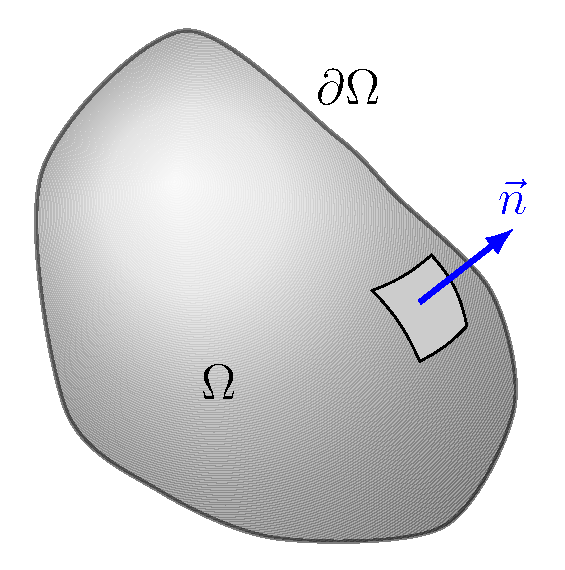
\includegraphics[scale=0.35]{Imagenes/Funcion_Green_01.png}
    \caption{Consideremos la ecuación de Poisson dentro de una región $\Omega$ acotada por una superficie $\partial \Omega$.}
    \label{fig:figura_07_01}
\end{figure}
Ahora pensemos en la fuente como una fuente puntual en la que estamos interesados en la respuesta del sistema a esta fuente puntual. Si la fuente puntual está ubicada en un punto $\vb{\pderivada{r}}$, entonces la respuesta a la fuente puntual podría sentirse en los puntos $\vb{r}$. Llamaremos a esta respuesta $G (\vb{r}, \vb{\pderivada{r}})$. La función de respuesta satisfaría una ecuación de fuente puntual de la forma:
\begin{align*}
\laplacian G (\vb{r}, \vb{\pderivada{r}}) = \delta (\vb{r} - \vb{\pderivada{r}})
\end{align*}
donde $\delta (\vb{r} - \vb{\pderivada{r}})$ es la función delta de Dirac. Una propiedad clave de esta función generalizada\footnote{Revisa el material de trabajo de la función delta de Dirac, en donde encontrarás varias propiedades, entre ellas, la propiedad de filtro.} es la propiedad de filtro:
\begin{align*}
\scaleint{6ex}_{\bs \Omega} \delta (\vb{r} - \vb{\pderivada{r}}) \, f (\vb{r}) \dd{V} = f (\vb{\pderivada{r}})
\end{align*}
La conexión entre la función de Green y la solución a la ecuación de Poisson se encuentra en la segunda identidad de Green:
\begin{align*}
\scaleint{6ex}_{\bs \partial \Omega} \bigg[ \phi \, \grad{\psi} - \psi \, \grad{\phi} \bigg] \cdot \vb{n} \dd{S} = \scaleint{6ex}_{\bs \Omega} \bigg[ \phi \, \laplacian{\psi} - \psi \, \laplacian{\phi} \bigg] \dd{V}
\end{align*}
Haciendo que $\phi = u (\vb{r})$ y $\psi = G (\vb{r}, \vb{\pderivada{r}})$, se tiene que\footnote{Considera que a continuación las integrales de volumen y de superficie, así como la diferenciación usando el operador $\grad$ se realizan usando las $\vb{r}$-coordenadas.}:
\begin{align}
\begin{aligned}[b]
\scaleint{6ex}_{\bs \partial \Omega} \bigg[ u (\vb{r}) \, \grad{G (\vb{r}, \vb{\pderivada{r}})} &- G (\vb{r}, \vb{\pderivada{r}}) \, \grad{u (\vb{r})} \bigg] \cdot \vb{n} \dd{S} = \\[0.5em]
&= \scaleint{6ex}_{\bs \Omega} \bigg[ u (\vb{r}) \, \laplacian{G (\vb{r}, \vb{\pderivada{r}})} - G (\vb{r}, \vb{\pderivada{r}}) \, \laplacian{u (\vb{r})} \bigg] \dd{V} = \\[0.5em]
&= \scaleint{6ex}_{\bs \Omega} \bigg[ u (\vb{r}) \, \delta (\vb{r} - \vb{\pderivada{r}}) - G (\vb{r}, \vb{\pderivada{r}}) \, f (\vb{r}) \bigg] \dd{V} = \\[0.5em]
&= u (\vb{\pderivada{r}}) - \scaleint{6ex}_{\bs \Omega} G (\vb{r}, \vb{\pderivada{r}}) \, f (\vb{r}) \dd{V}
\end{aligned}
\label{eq:ecuacion_07_02}
\end{align}
Al resolver para $u (\vb{\pderivada{r}})$, se tiene que:
\begin{align}
\begin{aligned}[b]
u (\vb{\pderivada{r}}) &= \scaleint{6ex}_{\bs \Omega} G (\vb{r}, \vb{\pderivada{r}}) \, f (\vb{r}) \dd{V} + \\[0.5em]
&+ \scaleint{6ex}_{\bs \partial \Omega} \bigg[ u (\vb{r}) \, \grad{G (\vb{r}, \vb{\pderivada{r}})} - G (\vb{r}, \vb{\pderivada{r}}) \, \grad{u (\vb{r})} \bigg] \cdot \vb{n} \dd{S}
\end{aligned}
\label{eq:ecuacion_07_03}
\end{align}
Si tanto $u (\vb{r})$ como $G (\vb{r}, \vb{\pderivada{r}})$ satisfacen las condiciones de Dirichlet, $u = 0$ en $\partial \Omega$, entonces la última integral se anula y nos queda\footnote{En algunas aplicaciones se presenta la simetría:
\begin{align*}
G (\vb{r}, \vb{\pderivada{r}}) = G (\vb{\pderivada{r}}, \vb{r})
\end{align*}
Por lo que el resultado se puede escribir como:
\begin{align*}
u (\vb{\pderivada{r}}) = \scaleint{6ex}_{\bs \Omega} G (\vb{r}, \vb{\pderivada{r}}) \, f (\vb{\pderivada{r}}) \dd{\pderivada{V}}
\end{align*}
}:
\begin{align*}
u (\vb{\pderivada{r}}) = \scaleint{6ex}_{\bs \Omega} G (\vb{r}, \vb{\pderivada{r}}) \, f (\vb{r}) \dd{V}
\end{align*}
Entonces, si conocemos la función de Green, podemos resolver la ecuación diferencial no homogénea. De hecho, podemos usar la función de Green para resolver problemas de valor límite y valor inicial no homogéneos.

\section{Funciones de Green para valores iniciales.}

En esta parte revisaremos la solución de problemas con valores iniciales que involucran ecuaciones diferenciales no homogéneas utilizando las funciones de Green.
\par
Nuestro objetivo es resolver la ecuación diferencial no homogénea:
\begin{align}
a (t) \, \sderivada{y} (t) + b (t) \, \pderivada{y} (t) + c (t) \, y (t) = f (t)
\label{eq:ecuacion_07_04}
\end{align}
sujeta a las condiciones iniciales:
\begin{align*}
y (0) = y_{0} \hspace{1cm} \pderivada{y} (0) = v_{0}
\end{align*}

Como estamos interesados en problemas de valor inicial, denotaremos la variable independiente como una variable temporal: $t$.
\par
La ec. (\ref{eq:ecuacion_07_04}) se puede escribir de forma compacta como:
\begin{align*}
L [y] = f
\end{align*}
donde $L$ es el operador diferencial:
\begin{align*}
L = a (t) \, \dv[2]{t} + b (t) \, \dv{t} + c (t) 
\end{align*}
Cuya solución está dada por:
\begin{align*}
y = L^{-1} [f]
\end{align*}
El inverso de un operador diferencial es un operador integral, que buscamos escribir en la forma:
\begin{align*}
y (t) = \scaleint{6ex} G (t, \tau) \, f(\tau) \dd{\tau}
\end{align*}
La función $G (t, \tau)$ se conoce como el  \emph{kernel} (núcleo) del operador integral y  se denomina función de Green.
\newpage
Tomando del curso de Ecuaciones Diferenciales I la parte de solución con el \emph{método de variación de parámetros\footnote{Recordemos que este método es un procedimiento útil para la obtención de una solución particular $y_{p} (x)$ de la EDO lineal (no homogénea) y se basa en el conocimiento de la solución general de la lineal homogénea asociada a dicha EDO lineal.}}, hacemos que:
\begin{align}
y_{p} (t) = c_{1} (t) \, y_{1} (t) + c_{2} (t) \, y_{2} (t)
\label{eq:ecuacion_07_05}
\end{align}
encontramos que tenemos que resolver el sistema de ecuaciones:
\begin{align}
\begin{aligned}[b]
\pderivada{c}_{1} (t) \, y_{1} (t) + \pderivada{c}_{2} (t) \, y_{2} (t) &= 0 \\[0.5em]
\pderivada{c}_{1} (t) \, \pderivada{y}_{1} (t) + \pderivada{c}_{2} (t) \, \pderivada{y}_{2} (t) &= \dfrac{f (t)}{q (t)}
\end{aligned}
\label{eq:ecuacion_07_06}
\end{align}
Este sistema se resuelve fácilmente, para obtener entonces:
\begin{align}
\begin{aligned}[b]
\pderivada{c}_{1} (t) &= - \dfrac{f (t) \, y_{2} (t)}{a (t) \big[ y_{1} (t) \, \pderivada{y}_{2} (t)  - \pderivada{y}_{1} (t) \, y_{2} (t) \big]} \\[0.5em]
\pderivada{c}_{2} (t) &= \dfrac{f (t) \, y_{1} (t)}{a (t) \big[ y_{1} (t) \, \pderivada{y}_{2} (t)  - \pderivada{y}_{1} (t) \, y_{2} (t) \big]}
\end{aligned}
\label{eq:ecuacion_07_07}
\end{align}
Notemos que el denominador en estas expresiones involucra el Wronskiano de las soluciones al problema homogéneo, el cual viene dado por el determinante:
\begin{align*}
W (y_{1}, y_{2}) (t) = \mqty|
y_{1} (t) & y_{2} (t) \\
\pderivada{y}_{1} (t) & \pderivada{y}_{2} (t) |
\end{align*}
Cuando $y_{1} (t)$ y $y_{2} (t)$ son linealmente independientes, entonces el Wronskiano no es cero y tenemos garantizada una solución para el sistema anterior.
\par
Entonces, después de una integración, encontramos los parámetros como:
\begin{align}
\begin{aligned}
c_{1} (t) &= - \scaleint{6ex}_{\bs t_{0}}^{t} \dfrac{f (\tau) \, y_{2} (\tau)}{a (\tau) \, W (\tau)} \dd{\tau} \\[0.5em]
c_{2} (t) &= \scaleint{6ex}_{\bs t_{1}}^{t} \dfrac{f (\tau) \, y_{1} (\tau)}{a (\tau) \, W (\tau)} \dd{\tau}
\end{aligned}
\label{eq:ecuacion_07_08}
\end{align}
donde $t_{0}$ y $t_{1}$ son constantes arbitrarias que se determinarán a partir de las condiciones iniciales.
\par
Por lo tanto, la solución particular de la ec. (\ref{eq:ecuacion_07_04}) se puede escribir como:
\begin{align}
y_{p} (t) = y_{2} (t) \scaleint{6ex}_{\bs t_{1}}^{t} \dfrac{f (\tau) \, y_{1} (\tau)}{a (\tau) \, W (\tau)} \dd{\tau} - y_{1} (t) \scaleint{6ex}_{\bs t_{0}}^{t} \dfrac{f (\tau) \, y_{2} (\tau)}{a (\tau) \, W (\tau)} \dd{\tau}
\label{eq:ecuacion_07_09}
\end{align}
Comenzamos con la solución particular de la ec. (\ref{eq:ecuacion_07_09}) de la ED no homogénea (\ref{eq:ecuacion_07_04}). Esto se puede combinar con la solución general del problema homogéneo para dar la solución general de la ecuación diferencial no homogénea:
\begin{align}
y_{p} (t) = c_{1} y_{1} (t) + c_{2} y_{2} (t) +  y_{2} (t) \scaleint{6ex}_{\bs t_{1}}^{t} \dfrac{f (\tau) \, y_{1} (\tau)}{a (\tau) \, W (\tau)} \dd{\tau} - y_{1} (t) \scaleint{6ex}_{\bs t_{0}}^{t} \dfrac{f (\tau) \, y_{2} (\tau)}{a (\tau) \, W (\tau)} \dd{\tau}
\label{eq:ecuacion_07_10}
\end{align}
Sin embargo, se puede encontrar una elección adecuada de $t_{0}$ y $t_{1}$ para que no necesitemos escribir explícitamente la solución al problema homogéneo, $c_{1} y_{1} (t) + c_{2} y_{2} (t)$. No obstante, configurar la solución de esta forma nos permitirá usar $t_{0}$ y $t_{1}$ para determinar soluciones particulares que satisfagan ciertas condiciones homogéneas. En particular, mostraremos que la ec. (\ref{eq:ecuacion_07_10}) se puede escribir en la forma:
\begin{align}
y_{p} (t) = c_{1} y_{1} (t) + c_{2} y_{2} (t) +  y_{2} (t) \scaleint{6ex}_{\bs 0}^{t} G (t,\tau) \, f (\tau) \dd{\tau}
\label{eq:ecuacion_07_11}
\end{align}
donde la función $G (t,\tau)$ será identificada como la función de Green.
\par
El objetivo es entonces desarrollar la técnica de la función de Green para resolver el problema de valor inicial:
\begin{align}
a (t) \, \sderivada{y} (t) + b (t) \, \pderivada{y} (t) + c (t) y(t) = f (t) \hspace{0.6cm} y (0) = y_{0}, \hspace{0.2cm} \pderivada{y} (0) = v_{0}
\label{eq:ecuacion_07_12}
\end{align}
Primero observamos que podemos resolver este problema de valores iniciales resolviendo dos problemas de valor inicial separados. Suponemos que la solución del problema homogéneo satisface las condiciones iniciales originales:
\begin{align}
a (t) \, \sderivada{y}_{h} (t) + b (t) \, \pderivada{y}_{h} (t) + c (t) y_{h} (t) = f (t) \hspace{0.6cm} y_{h} (0) = y_{0}, \hspace{0.2cm} \pderivada{y}_{h} (0) = v_{0}
\label{eq:ecuacion_07_13}
\end{align}
Entonces asumimos que la solución particular satisface el problema:
\begin{align}
a (t) \, \sderivada{y}_{p} (t) + b (t) \, \pderivada{y}_{p} (t) + c (t) y_{h} (t) = f (t) \hspace{0.6cm} y_{p} (0) = y_{0}, \hspace{0.2cm} \pderivada{y}_{p} (0) = v_{0}
\label{eq:ecuacion_07_14}
\end{align}

Dado que la ecuación diferencial es lineal, se sabe que:
\begin{align*}
y (t) = y_{h} (t) + y_{p} (t)
\end{align*}
es una solución a la ecuación no homogénea. También, esta solución satisface las condiciones iniciales:
\begin{align*}
y (0) &= y_{h} (0) + y_{p} (0) = y_{0} + 0 = y_{0} \\[0.5em]
\pderivada{y} (0) &= \pderivada{y}_{h} (0) + \pderivada{y}_{p} (0) = v_{0} + 0 = v_{0}
\end{align*}
Por lo tanto, solo debemos centrarnos en encontrar una solución particular que satisfaga las condiciones iniciales homogéneas. Esto se hará encontrando valores para $t_{0}$ y $t_{1}$ en la ec. (\ref{eq:ecuacion_07_09}) que satisfagan las condiciones iniciales homogéneas: $y_{p} (0) = 0$ y $\pderivada{y}_{p} (0) = 0$
\par
Primero, consideramos $y_{p} (0) = 0$. Tenemos que:
\begin{align}
y_{p} (0) = y_{2} (0) \scaleint{6ex}_{\bs t_{1}}^{0} \dfrac{f (\tau) \, y_{1} (\tau)}{a (\tau) \, W (\tau)} \dd{\tau} - y_{1} (0) \scaleint{6ex}_{\bs t_{0}}^{t} \dfrac{f (\tau) \, y_{2} (\tau)}{a (\tau) \, W (\tau)} \dd{\tau}
\label{eq:ecuacion_07_15}
\end{align}
Aquí, $y_{1} (t)$ y $y_{2} (t)$ se toman como cualquier solución de la ecuación diferencial homogénea. Supongamos que $y_{1} (0) = 0$ y $y_{2} (0) \neq 0$. Entonces, tenemos:
\begin{align}
y_{p} (0) = y_{2} (0) \scaleint{6ex}_{\bs t_{1}}^{0} \dfrac{f (\tau) \, y_{1} (\tau)}{a (\tau) \, W (\tau)} \dd{\tau}
\label{eq:ecuacion_07_16}
\end{align}
Podemos forzar que $y_{p} (0) = 0$ si hacemos que $t_{1} = 0$.
\par
Ahora, consideramos $\pderivada{y}_{p} (0) = 0$. Primero derivamos la solución y encontramos que:
\begin{align}
\pderivada{y}_{p} (t) = \pderivada{y}_{2} (t) \scaleint{6ex}_{\bs 0}^{t} \dfrac{f (\tau) \, y_{1} (\tau)}{a (\tau) \, W (\tau)} \dd{\tau} - \pderivada{y}_{1} (t) \scaleint{6ex}_{\bs t_{0}}^{t} \dfrac{f (\tau) \, y_{2} (\tau)}{a (\tau) \, W (\tau)} \dd{\tau}
\label{eq:ecuacion_07_17}
\end{align}
ya que las contribuciones al diferenciar las integrales se cancelarán. Evaluando este resultado en $t = 0$, tenemos:
\begin{align}
\pderivada{y}_{p} (0) = - \pderivada{y}_{1} (0) \scaleint{6ex}_{\bs t_{0}}^{0} \dfrac{f (\tau) \, y_{2} (\tau)}{a (\tau) \, W (\tau)} \dd{\tau}
\label{eq:ecuacion_07_18}
\end{align}
Suponiendo que $\pderivada{y}_{p} (0) \neq 0$, podemos hacer que $t_{0} = 0$.
\par
Entonces, hemos encontrado que:
\begin{align}
\begin{aligned}[b]
y_{p} (x) &= y_{2} (t) \scaleint{6ex}_{\bs 0}^{t} \dfrac{f (\tau) \, y_{1} (\tau)}{a (\tau) \, W (\tau)} \dd{\tau} - y_{1} (t) \scaleint{6ex}_{\bs t_{0}}^{t} \dfrac{f (\tau) \, y_{2} (\tau)}{a (\tau) \, W (\tau)} \dd{\tau} = \\[0.5em]
&= \scaleint{6ex}_{\bs 0}^{t} \bigg[ \dfrac{y_{1} (\tau) \, y_{2} (t) - y_{1} (t) \, y_{2} (\tau)}{a (\tau) \, W (\tau)} \bigg] \, f (\tau) \dd{\tau}
\end{aligned}
\label{eq:ecuacion_07_19}
\end{align}
Este resultado está en la forma correcta y podemos identificar el valor temporal o inicial: la función de Green. Entonces, la solución particular se da como:
\begin{align}
y_{p} (t) = \scaleint{6ex}_{\bs 0}^{t} G (t, \tau) \, f (\tau) \dd{\tau}
\label{eq:ecuacion_07_20}
\end{align}
donde la condición inicial de la función de Green está definida como:
\begin{align*}
G (t, \tau) = \dfrac{y_{1} (\tau) \, y_{2} (t) - y_{1} (t) \, y_{2} (\tau)}{a (\tau) \, W (\tau)}
\end{align*}

A modo de resumen:
\begin{tcolorbox}[title={\centering Solución para problema de valores iniciales con la función de Green}]

La solución al problema de valores iniciales:
\begin{align*}
a (t) \, \sderivada{y} (t) + b (t) \pderivada{y} (t) + c (t) \, y (t) = f (t) \hspace{0.6cm} y (0) = y_{0}, \hspace{0.2cm} \pderivada{y} (0) = v_{0}
\end{align*}
es de la forma:
\begin{align}
y (t) = y_{h} (t) + \scaleint{6ex}_{\bs 0}^{t} G (t, \tau) \, f (t) \dd{\tau}
\label{eq:ecuacion_07_21}
\end{align}
donde:
\begin{align}
G (t, \tau) = \dfrac{y_{1} (\tau) \, y_{2} (t) - y_{1} (t) \, y_{2} (\tau)}{a (\tau) \, W (\tau)}
\label{eq:ecuacion_07_22}
\end{align}
es la función de Green, $y_{1}$, $y_{2}$, $y_{h}$ son soluciones de la ecuación homogénea que satisfacen:
\begin{align*}
y_{1} (0) = 0, \hspace{0.2cm} y_{2} (0) \neq 0, \hspace{0.2cm} \pderivada{y}_{1} (0) \neq 0, \hspace{0.2cm} \pderivada{y}_{2} (0) = 0, \hspace{0.2cm} y_{h} (0) = y_{0}, \hspace{0.2cm} \pderivada{y}_{h} (0) = v_{0}
\end{align*}
\end{tcolorbox}
\begin{ejemplo}
Resolvamos el problema del oscilador forzado:
\begin{align*}
\sderivada{x} + x = 2 \, \cos t, \hspace{0.5cm} x (0) = 4, \hspace{0.2cm} \pderivada{x} (0) = 0
\end{align*}
Primero resolvemos el problema homogéneo con las condiciones iniciales no homogéneas:
\begin{align*}
\sderivada{x}_{h} + x_{h} = 0, \hspace{0.5cm} x_{h} (0) = 4, \hspace{0.2cm} \pderivada{x}_{h} (0) = 0
\end{align*}
Cuya solución se obtiene fácilmente: $x_{h} (t) = 4 \, \cos t$, que se presenta en la figura (\ref{fig:figura_01}).
\par
A continuación, construimos la función de Green. Necesitamos dos soluciones linealmente independientes, $y_{1} (x)$, $y_{2} (x)$, para la ecuación diferencial homogénea que satisfaga diferentes condiciones homogéneas, $y_{1} (0) = 0$ y $\pderivada{y}_{2} (0) = 0$. Las soluciones más simples son $y_{1} (t) = \sen t$ y $y_{2} (t) = \cos t$.
\par
El Wronskiano para este ejemplo es:
\begin{align*}
W (t) = y_{1} (t) \, \pderivada{y}_{2} (t) - \pderivada{y}_{1} (t) \, y_{2} (t) = - \sin^{2} (t) - \cos^{2} (t) = - 1 
\end{align*}
Dado que en este ejercicio $a (t) = 1$, es posible calcular la función de Green:
\begin{align}
\begin{aligned}[b]
G (t, \tau) &= G (t, \tau) = \dfrac{y_{1} (\tau) \, y_{2} (t) - y_{1} (t) \, y_{2} (\tau)}{a (\tau) \, W (\tau)} = \\[0.5em]
&= \sin t \, \cos \tau - \sin \tau \, \cos t = \\[0.5em]
&= \sin (t - \tau)
\end{aligned}
\label{eq:ecuacion_07_23}
\end{align}
Tomemos en cuenta que la función de Green depende de $t - \tau$. Si bien esto es útil en algunos contextos, usaremos la forma expandida al realizar la integración.
\par
Ahora podemos determinar la solución particular de la ecuación diferencial no homogénea. Tenemos que:
\begin{align}
\begin{aligned}[b]
x_{p} (t) &= \scaleint{6ex}_{\bs 0}^{t} G (t, \tau) \, f (\tau) \dd{\tau} = \\[0.5em]
&= \scaleint{6ex}_{\bs 0}^{t} (\sin t \, \cos \tau - \sin \tau \, \cos t) (2 \, \cos \tau) \dd{\tau} = \\[0.5em]
&= 2 \sin t \, \scaleint{6ex}_{\bs 0}^{t} \cos^{2} \tau \dd{\tau} - 2 \cos t \, \scaleint{6ex}_{\bs 0}^{t} \sin \tau \, \cos \tau \dd{\tau} = \\[0.5em]
&= 2 \sin t \, \bigg[ \dfrac{\tau}{2} + \dfrac{1}{2} \, \sin 2 \tau \bigg] \eval_{0}^{t} - 2 \cos t \, \bigg[ \dfrac{1}{2} \, \sin^{2} \tau \bigg] \eval_{0}^{t} = \\[0.5em]
&= t \, \sin t
\end{aligned}
\label{eq:ecuacion_07_24}
\end{align}

En la figura (\ref{fig:figura_01}) se muestran las soluciones al caso homogéneo como no homogéneo.
\begin{figure}[H]
    \centering
    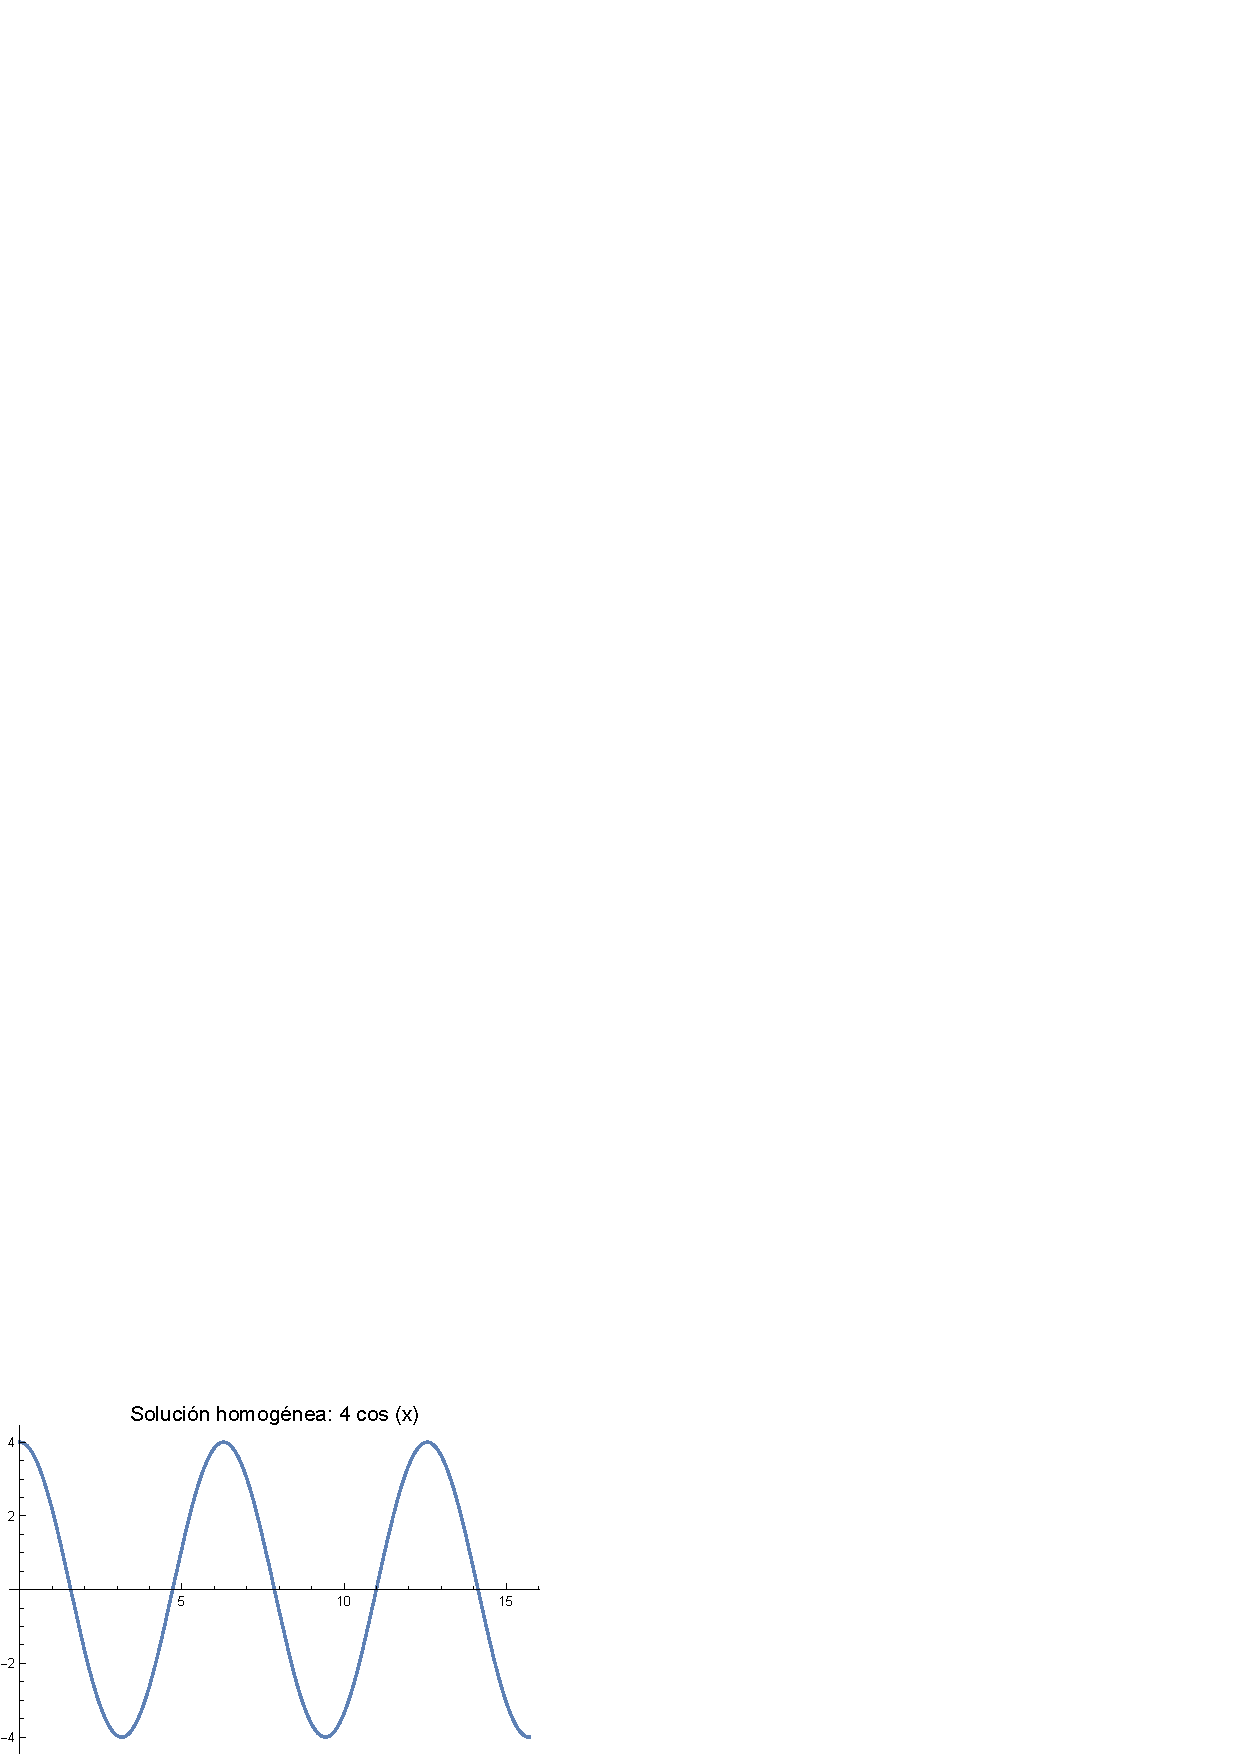
\includegraphics[scale=0.75]{Imagenes/Plot_Oscilador_Forzado_Green_01.pdf}
    \caption{Soluciones a la EDO en el caso homogéneo y no homogéneo.}
    \label{fig:figura_01}
\end{figure}

Por lo tanto, la solución al problema no homogéneo, es la suma es la solución del problema homogéneo y esta solución particular:
\begin{align*}
x (t) = 4 \, \cos t + t \, \sin t
\end{align*}
La gráfica de la solución se muestra en la figura (\ref{fig:figura_02}):
\begin{figure}[H]
    \centering
    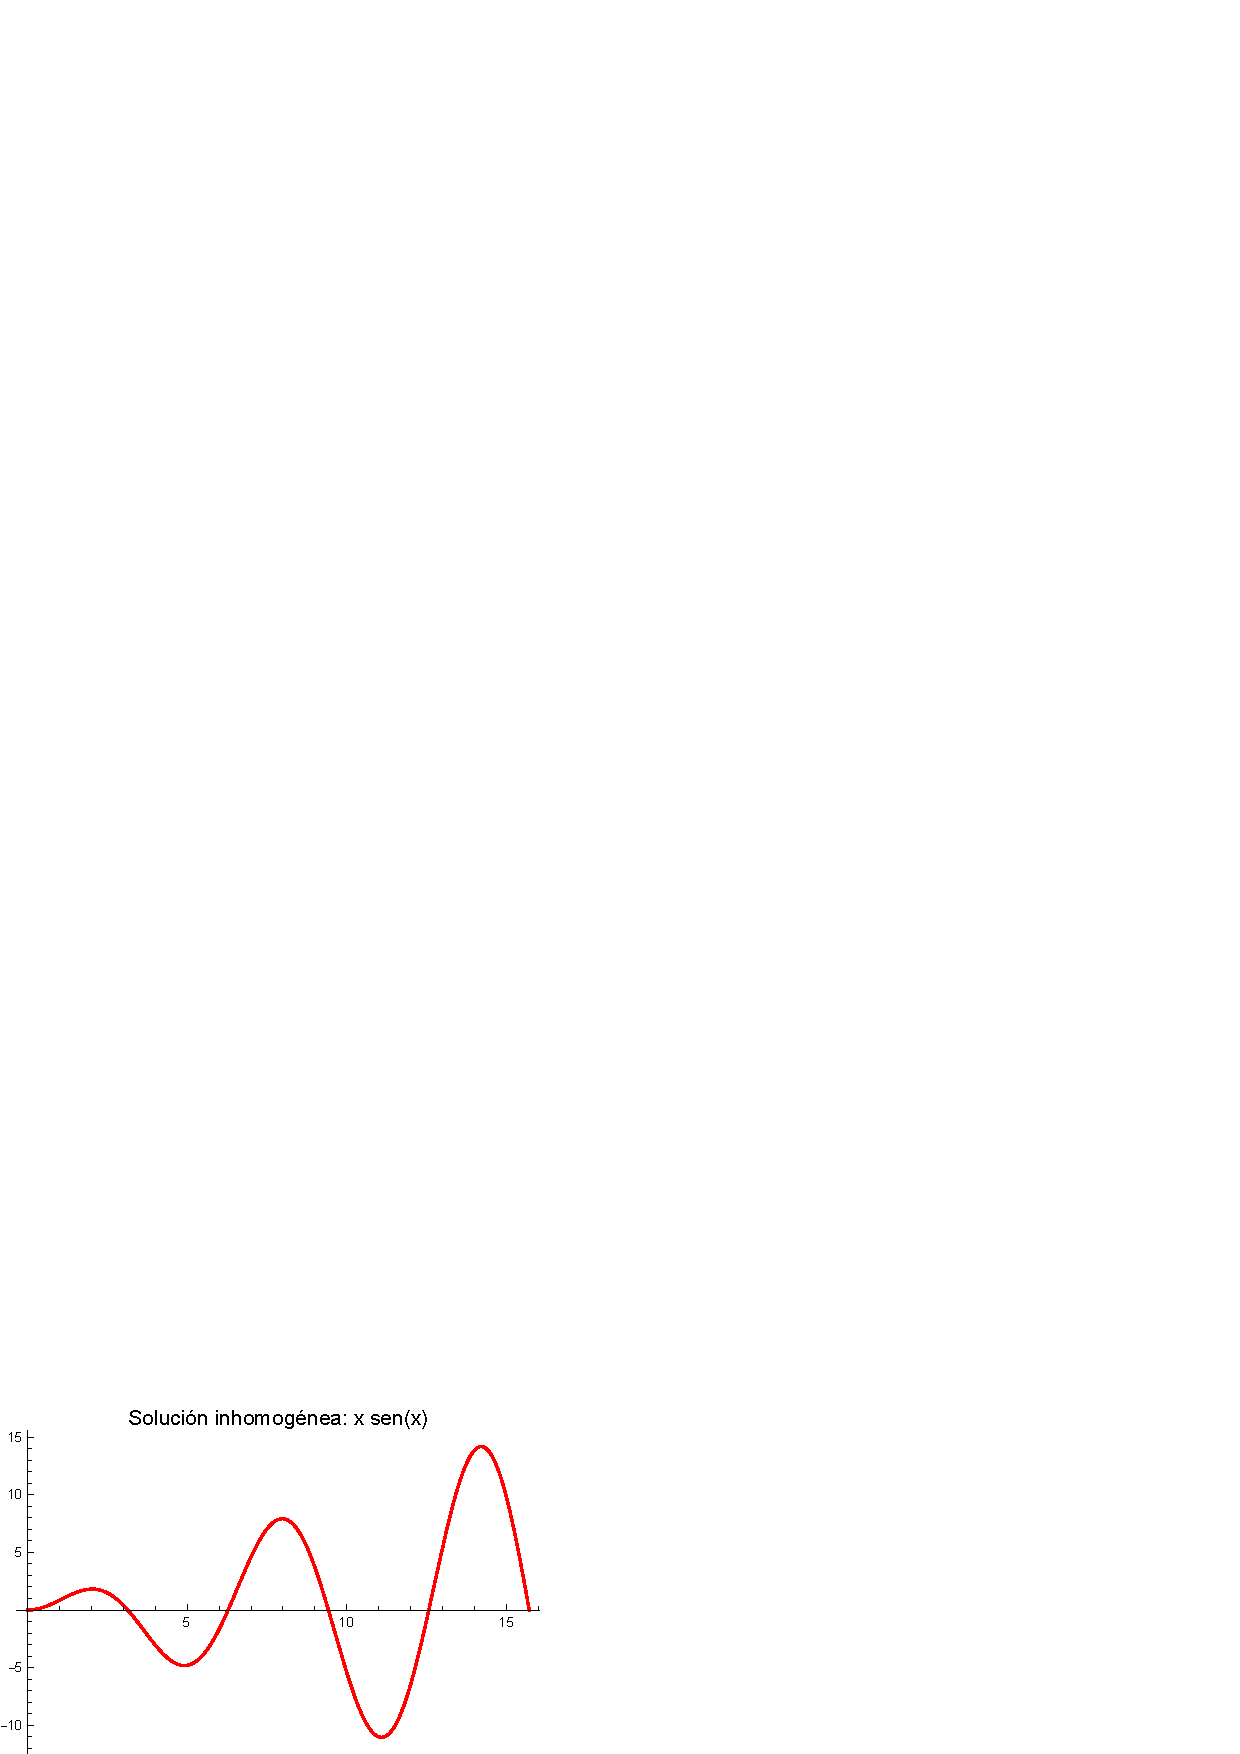
\includegraphics[scale=0.8]{Imagenes/Plot_Oscilador_Forzado_Green_02.pdf}
    \caption{Solución completa a la EDO no homogénea.}
    \label{fig:figura_02}
\end{figure}

\end{ejemplo}

\section{Valores de frontera y funciones de Green.}

En el numeral anterior, resolvimos problemas de valores iniciales no homogéneos usando una función de Green. En esta sección extenderemos este método a la solución de problemas de valores en la frontera no homogéneos usando una función de Green. Recordemos que el objetivo es resolver la ecuación diferencial no homogénea:
\begin{align*}
L [y] = f, \hspace{0.6cm} a \leq x \leq b
\end{align*}
donde $L$ es un operador diferencial y $y (x)$ satisface las condiciones de frontera en $x = a$ y $x = b$. La solución viene dada formalmente por:
\begin{align*}
y = L^{-1} [y]
\end{align*}

El \emph{inverso de un operador diferencial es un operador integral}, que buscamos escribir de la forma:
\begin{align*}
y (x) = \scaleint{6ex}_{a}^{b} G (x, \xi) \, f (\xi) \dd{\xi} 
\end{align*}
La función $G (x, \xi)$ se conoce como el \emph{kernel} (núcleo) del operador integral y se le llama \emph{función de Green}.
\par
Consideraremos problemas de valores en la frontera en forma de Sturm-Liouville\footnote{Este concepto será la parte central del contenido del Tema 3, que sin pérdida de generalidad, podemos mencionar en este momento.}:
\begin{align}
\dv{x} \bigg[ p (x) \, \dv{y (x)}{x} \bigg] + q (x) \, y (x) = f (x), \hspace{0.6cm} a < x < b
\label{eq:ecuacion_07_25}
\end{align}
con valores fijos de $y (x)$ en la frontera, $y (a) = 0$ y $y (b) = 0$. Sin embargo, la teoría general funciona para otras formas de condiciones de frontera homogéneas.
\par
Buscamos la función de Green resolviendo primero la ecuación diferencial no homogénea usando el método de variación de parámetros. Suponemos una solución particular de la forma
\begin{align*}
y_{p} (x) = c_{1} (x) \, y_{1} (x) + c_{2} (x) \, y_{2} (x)
\end{align*}
que se forma a partir de dos soluciones linealmente independientes del problema homogéneo, $y_{i} (x), i = 1, 2$. Habíamos encontrado que las funciones de los coeficientes satisfacen las ecuaciones:
\begin{align}
\begin{aligned}[b]
\pderivada{c}_{1} (t) \, y_{1} (t) + \pderivada{c}_{2} (t) \, y_{2} (t) &= 0 \\[0.5em]
\pderivada{c}_{1} (t) \, \pderivada{y}_{1} (t) + \pderivada{c}_{2} (t) \, \pderivada{y}_{2} (t) &= \dfrac{f (t)}{q (t)}
\end{aligned}
\label{eq:ecuacion_07_26}
\end{align}
resolviendo este sistema, se obtiene:
\begin{align*}
\pderivada{c}_{1} (x) &= - \dfrac{f \, y_{2}}{p \, W (y_{1}, y_{2})} \\[0.5em]
\pderivada{c}_{2} (x) &= \dfrac{f \, y_{1}}{p \, W (y_{1}, y_{2})}
\end{align*}
donde $W (y_{1}, y_{2}) = y_{1} \, \pderivada{y}_{2} - \pderivada{y}_{1} \, y_{2}$ es el Wronskiano. Integrando las expresiones para sustituirlas de regreso en la solución particular, se encuentra que:
\begin{align*}
y (x) = y_{2} (x) \scaleint{6ex}_{\bs x_{1}}^{x_{2}} \dfrac{f (\xi) \, y_{1} (\xi)}{p (\xi) \, W (\xi)} \dd{\xi} - y_{1} (x) \scaleint{6ex}_{\bs x_{0}}^{x} \dfrac{f (\xi) \, y_{2} (\xi)}{p (\xi) \, W (\xi)} \dd{\xi}
\end{align*}
donde $x_{0}$ y $x_{1}$ se determinarán utilizando las condiciones de frontera. En particular, buscaremos $x_{0}$ y $x_{1}$ para que la solución al problema de valores en la frontera pueda escribirse como una integral simple que involucre una función de Green. %Notemos que podemos absorber la solución del problema homogéneo, yh(x), en las integrales con una elección apropiada de límites en las integrales.
\par
Ahora buscamos satisfacer las condiciones $y (a) = 0$ y $y (b) = 0$. Primero usamos soluciones de la ecuación diferencial homogénea que satisfacen $y_{1} (a) = 0$, $y_{2} (b) = 0$ y $y_{1} (b) \neq 0$, $y_{2} (a) \neq 0$. Evaluando $y (x)$ en $x = 0$, tenemos que:
\begin{align}
\begin{aligned}[b]
y (a) &= y_{2} (a) \scaleint{6ex}_{\bs x_{1}}^{a} \dfrac{f (\xi) \, y_{1} (\xi)}{p (\xi) \, W (\xi)} \dd{\xi} - y_{1} (a) \scaleint{6ex}_{\bs x_{0}}^{a} \dfrac{f (\xi) \, y_{2} (\xi)}{p (\xi) \, W (\xi)} \dd{\xi} = \\[0.5em]
&= y_{2} (a) \scaleint{6ex}_{\bs x_{1}}^{a} \dfrac{f (\xi) \, y_{1} (\xi)}{p (\xi) \, W (\xi)} \dd{\xi}
\end{aligned}
\label{eq:ecuacion_07_27}
\end{align}
Podemos satisfacer la condición en $x = a$ si escogemos $x_{1} = a$. De manera similar, en $x = b$, encontramos que:
\begin{align}
\begin{aligned}[b]
y (b) &= y_{2} (b) \scaleint{6ex}_{\bs x_{1}}^{b} \dfrac{f (\xi) \, y_{1} (\xi)}{p (\xi) \, W (\xi)} \dd{\xi} - y_{1} (b) \scaleint{6ex}_{\bs x_{0}}^{b} \dfrac{f (\xi) \, y_{2} (\xi)}{p (\xi) \, W (\xi)} \dd{\xi} = \\[0.5em]
&= - y_{1} (b) \scaleint{6ex}_{\bs x_{0}}^{b} \dfrac{f (\xi) \, y_{2} (\xi)}{p (\xi) \, W (\xi)} \dd{\xi}
\end{aligned}
\label{eq:ecuacion_07_28}
\end{align}
Esta expresión se anula para $x_{0} = b$.

Así, hemos encontrado que la solución es de la forma:
\begin{align}
y (x) &= y_{2} (x) \scaleint{6ex}_{\bs a}^{x} \dfrac{f (\xi) \, y_{1} (\xi)}{p (\xi) \, W (\xi)} \dd{\xi} - y_{1} (x) \scaleint{6ex}_{\bs b}^{x} \dfrac{f (\xi) \, y_{2} (\xi)}{p (\xi) \, W (\xi)} \dd{\xi}
\label{eq:ecuacion_07_29}
\end{align}
Esta solución se puede escribir en forma compacta tal como lo hicimos para el problema de valores iniciales del numeral anterior. Buscamos una función de Green para que la solución se pueda escribir como una sola integral. Podemos mover las funciones de $x$ debajo de la integral. Además, dado que $a < x < b$, podemos invertir los límites en la segunda integral. Esto nos da:
\begin{align}
y (x) &= \scaleint{6ex}_{\bs x}^{a} \dfrac{f (\xi) \, y_{1} (\xi) \, y_{2} (x)}{p (\xi) \, W (\xi)} \dd{\xi} + \scaleint{6ex}_{\bs x}^{b} \dfrac{f (\xi) \, y_{1} (x) \, y_{2} (\xi)}{p (\xi) \, W (\xi)} \dd{\xi}
\label{eq:ecuacion_07_30}
\end{align}
Este resultado se puede ahora escribir de una manera compacta:
\begin{tcolorbox}[title={\centering Solución para problema de CDF con la función de Green}]

La solución para el problema de condiciones de frontera:
\begin{align}
\begin{aligned}
\dv{x} \bigg[ p (x) \, \dv{y (x)}{x} \bigg] &+ q (x) \, y (x) = f (x), \hspace{0.6cm} a < x < b \\[0.5em]
&y (a) = 0, \hspace{0.4cm} y (b) = 0
\end{aligned}
\label{eq:ecuacion_07_31}
\end{align}
toma la forma:
\begin{align}
y (x) = \scaleint{6ex}_{\bs a}^{b} G (x, \xi) \, f (\xi) \dd{\xi}
\label{eq:ecuacion_07_32}
\end{align}
donde la función de Green es una función en partes definida como:
\begin{align}
G (x, \xi) = \begin{cases}
\dfrac{y_{1} (\xi) \, y_{2} (x)}{p \, W}, & a \leq \xi \leq x \\[0.5em]
\dfrac{y_{1} (x) \, y_{2} (\xi)}{p \, W}, & x \leq \xi \leq b
\end{cases}
\label{eq:ecuacion_07_33}
\end{align}
donde $y_{1} (x)$ y $y_{2} (x)$ son soluciones al problema homogéneo que satisfacen $y_{1} (a) = 0$, $y_{2} (b) = 0$ y $y_{1} (b) \neq 0$, $y_{2} (a) \neq 0$.
\end{tcolorbox}

La función de Green satisface varias propiedades, que revisaremos más adelante. Por ejemplo, la función de Green satisface las condiciones de frontera en $x = a$ y $x = b$. Por lo tanto:
\begin{align*}
G (a, \xi) &= \dfrac{y_{1} (a) \, y_{2} (x)}{p \, W} = 0 \\[0.5em]        
G (b, \xi) &= \dfrac{y_{1} (\xi) \, y_{2} (b)}{p \, W} = 0
\end{align*}
Además, la función de Green es simétrica en sus argumentos. Intercambiando los argumentos nos devuelve:
\begin{align}
G (\xi, x) = \begin{cases}
\dfrac{y_{1} (x) \, y_{2} (\xi)}{p \, W}, & a \leq x \leq \xi \\[0.5em]
\dfrac{y_{1} (\xi) \, y_{2} (x)}{p \, W}, & \xi \leq x \leq b
\end{cases}
\label{eq:ecuacion_07_34}
\end{align}    
Pero revisando de manera cuidadosa a la forma original, tenemos que:
\begin{align*}
G (x, \xi) = G (\xi, x)
\end{align*}

Haremos uso de estas propiedades más adelante para determinar rápidamente las funciones de Green para otros problemas de valores en la frontera.

\begin{ejemplo}
Usando la función de Green para CDF, resuelve el problema:
\begin{align*}
\sderivada{y} = x^{2}, \hspace{0.6cm} y (0) = 0 = y (1)
\end{align*}
Primero resolvemos la ecuación homogénea, $\sderivada{y} = 0$. Después de dos integraciones, tenemos que:
\begin{align*}
y (x) = A \, x + B
\end{align*}
donde falta determinar las constantes $A$ y $B$.
\par
Necesitamos una solución que satisfaga $y_{1} (0) = 0$. Por lo tanto:
\begin{align*}
0 = y_{1} (0) = B
\end{align*}

\end{ejemplo}
Entonces, podemos elegir $y_{1} (x) = x$, ya que $A$ es arbitrario.
\par
La otra solución tiene que satisfacer $y_{2} (1) = 0$. Entonces:
\begin{align*}
0 = y_{2} (1) = A + B
\end{align*}
Esto se puede resolver para $B = - A$. Nuevamente, $A$ es arbitraria y elegimos $A = - 1$. Por tanto:
\begin{align*}
y_{2} (x) = 1 - x
\end{align*}
Las soluciones al problema homogéneo se presentan en la figura (\ref{fig:figura_03}).
\begin{figure}[H]
    \centering
    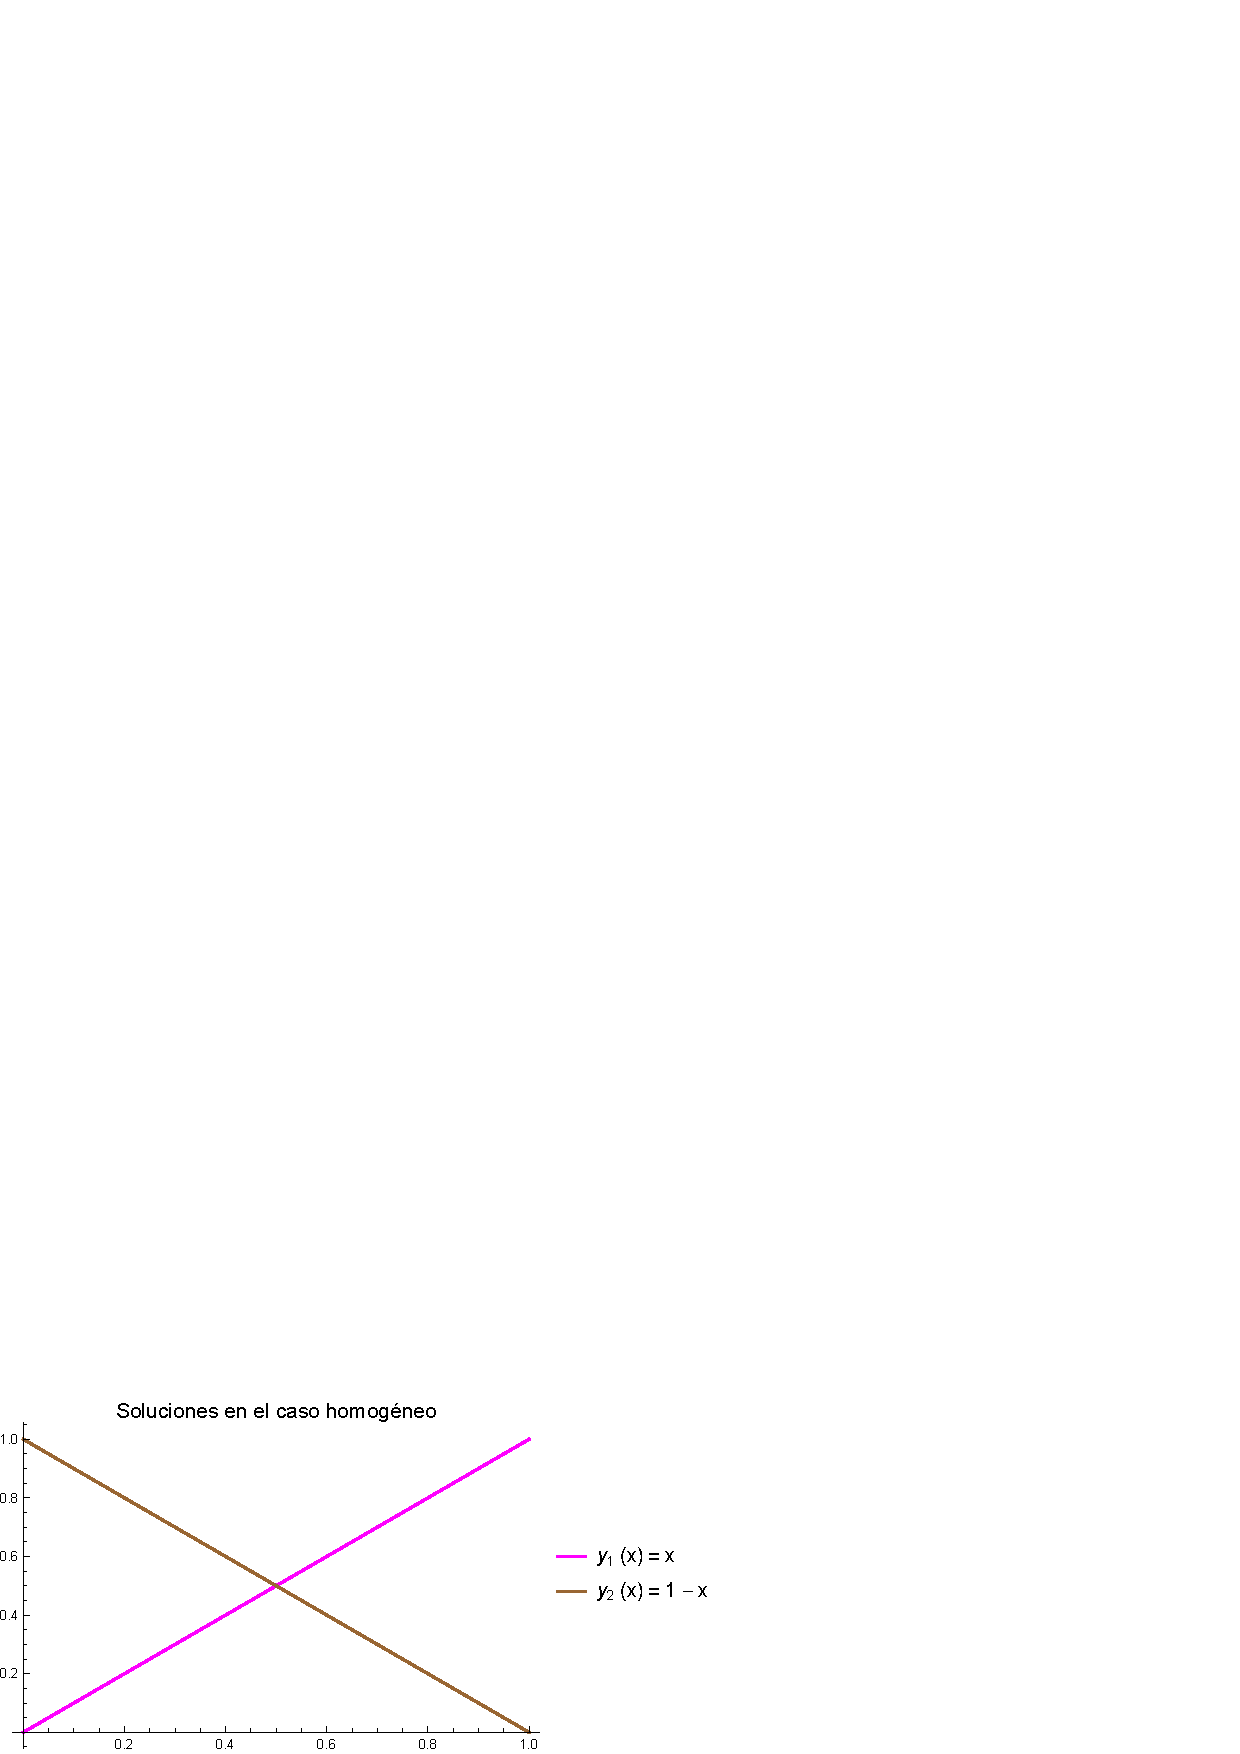
\includegraphics[scale=0.75]{Imagenes/Plot_EDONH_Green_01.pdf}
    \caption{Soluciones $y_{1} (x)$ y $y_{2} (x)$ para el caso de la ED homogénea.}
    \label{fig:figura_03}
\end{figure}

Para este problema $p (x) = 1$. Así, para $y_{1} (x) = x$ y $y_{2} (x) = 1 - x$, el producto:
\begin{align*}
p (x) \, W (x) =  y_{1} (x) \, \pderivada{y}_{2} (x) - \pderivada{y}_{1} (x) \, y_{2} (x) = x (-1) -  1(1 - x) = - 1
\end{align*}
Tomemos en cuenta que $p (x) \, W (x)$ es una constante, como debería ser.
\par
Ahora construimos la función de Green. Así tenemos:
\begin{align}
G (x, \xi) = \begin{cases}
- \xi \, (1 - x), & 0 \leq \xi \leq x \\
- x \, (1 - \xi), & x \leq \xi \leq 1
\end{cases}
\label{eq:ecuacion_07_35}
\end{align}

Observemos la simetría entre las dos partes de la función de Green. \break \hfill Además, la función de Green satisface condiciones de frontera homogéneas: 
\begin{align*}
G (0, \xi) &= 0, \mbox{ de la parte inferior}, \\[0.5em]
G (1, \xi) &= 0, \mbox{ de la parte superior}
\end{align*}
Finalmente, sustituimos la función de Green en la forma integral de la solución y evaluamos la integral:
\begin{align}
\begin{aligned}[b]
y (x) &= \scaleint{6ex}_{0}^{1} G (x, \xi) \, f (\xi) \dd{\xi} = \\[0.5em]
&= \scaleint{6ex}_{0}^{1} G (x, \xi) \, \xi^{2} \dd{\xi} = \\[0.5em]
&= - \scaleint{6ex}_{0}^{x} \xi \, (1 - x) \, \xi^{2} \dd{\xi} - \scaleint{6ex}_{x}^{1} x \, (1 - \xi) \, \xi^{2} \dd{\xi} = \\[0.5em]
&= - (1 - x) \scaleint{6ex}_{0}^{x} \xi^{3} \dd{\xi} - x \, \scaleint{6ex}_{x}^{1} (\xi^{2} - \xi^{3}) \dd{\xi} = \\[0.5em]
&= - (1 - x) \bigg[ \dfrac{\xi^{4}}{4} \bigg] \eval_{0}^{4} - x \bigg[ \dfrac{\xi^{3}}{3} - \dfrac{\xi^{4}}{4} \bigg] \eval_{x}^{1} = \\[0.5em]
&= \dfrac{1}{4} (1 - x) x^{4} - \dfrac{1}{12} \, x (4 - 3) + \dfrac{1}{12} \, x (4 x^{3} - 3 x^{4}) = \\[0.5em]
&= \dfrac{1}{12} (x^{4} - x)
\end{aligned}
\label{eq:ecuacion_07_36}
\end{align}
Revisando la solución, se verifica fácilmente que la EDO
\begin{align*}
\sderivada{y} = x^{2}
\end{align*}
se satisface para las CDF $y (0) = 0$ y $y (1) = 0$. La solución completa al caso no homogéneo se presenta en la figura (\ref{fig:figura_04}).
\begin{figure}[H]
    \centering
    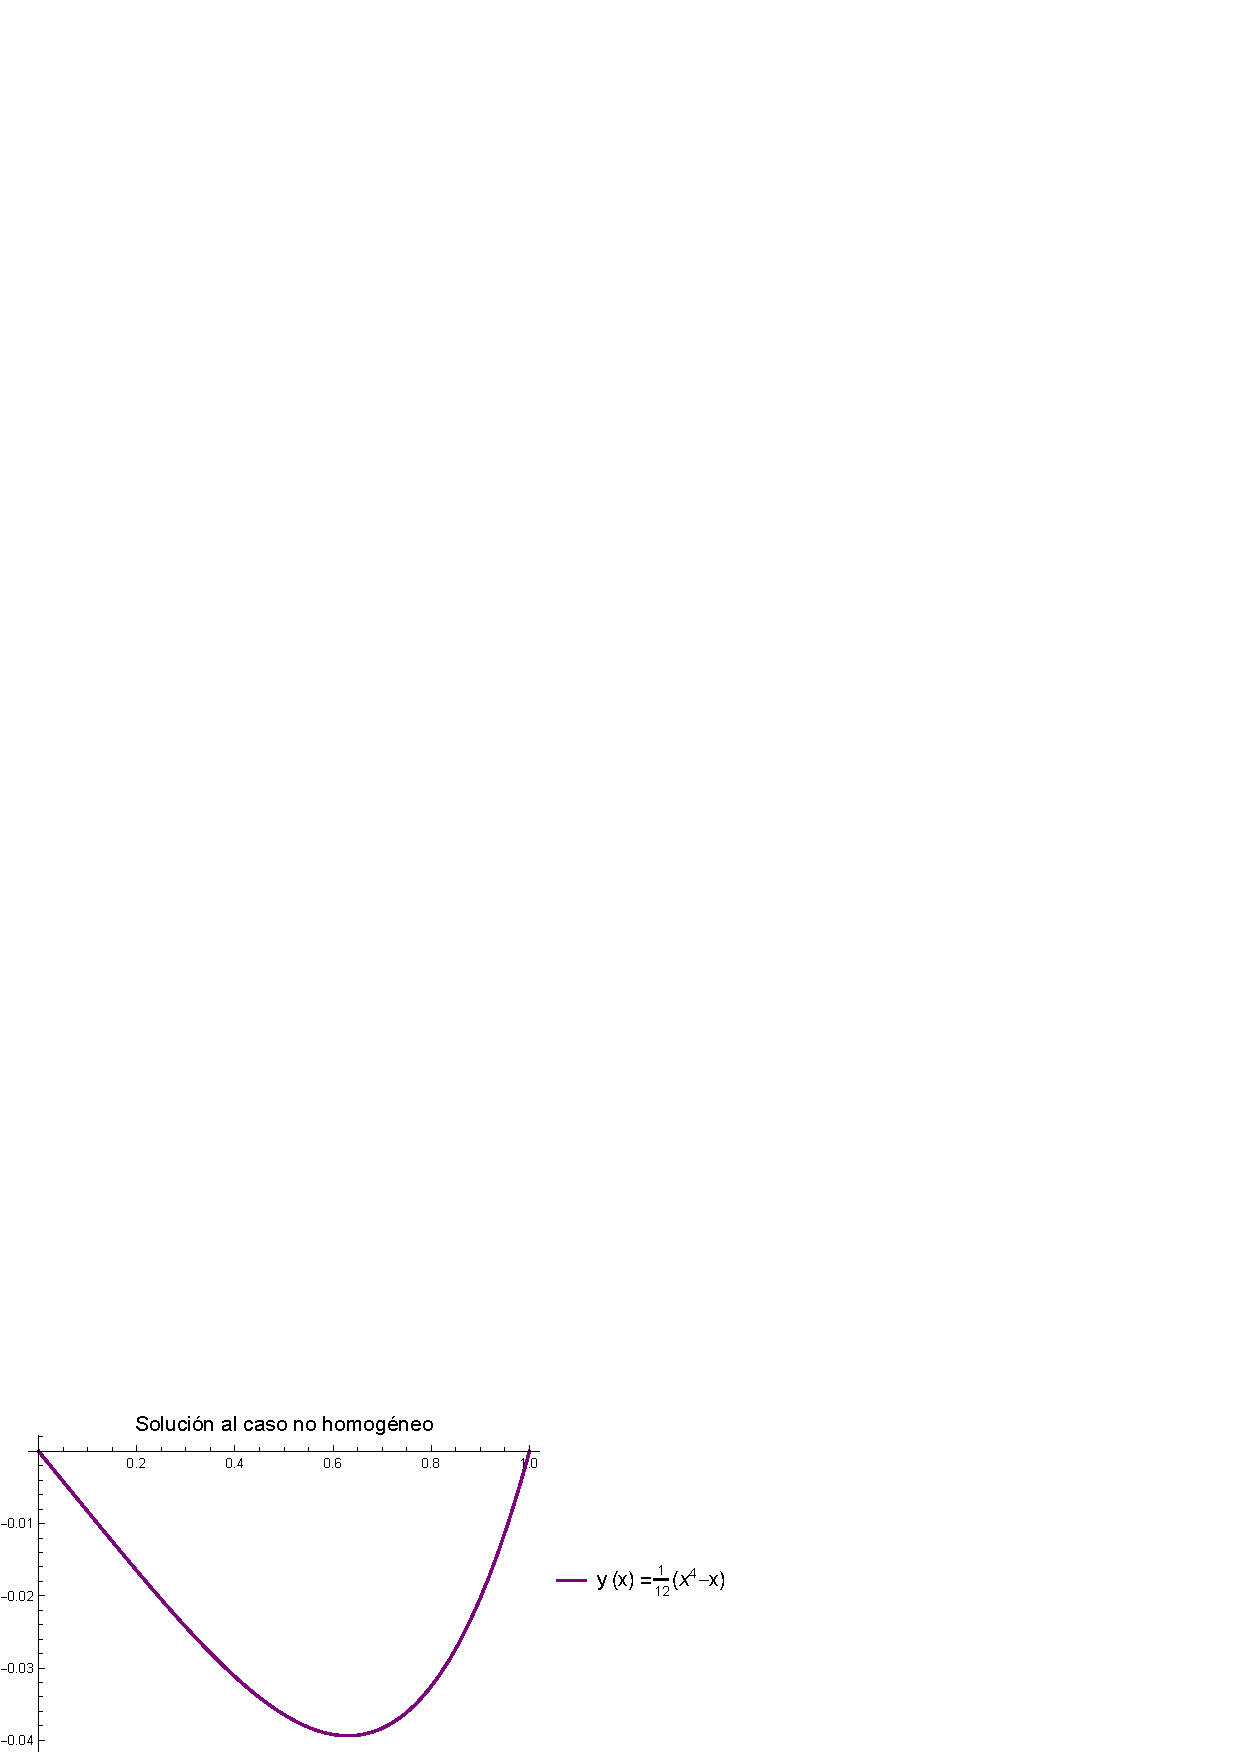
\includegraphics[scale=0.75]{Imagenes/Plot_EDONH_Green_02.pdf}
    \caption{Solución a la ED no homogénea que cumple con las CDF indicadas en el ejercicio.}
    \label{fig:figura_04}
\end{figure}

\section{Propiedades de la función de Green.}

Hemos mencionado algunas propiedades de las funciones de Green en el último numeral.
\par
En esta parte revisaremos algunas de estas propiedades como una herramienta para construir rápidamente funciones de Green para problemas de valores en la frontera. Enumeramos cinco propiedades básicas:
\begin{enumerate}
\item \textbf{Ecuación diferencial: } La función de Green con valor de frontera satisface la ecuación diferencial:
\begin{align*}
\pdv{x} \bigg[ p (x) \, \pdv{G (x, \xi)}{x} \bigg] + q (x) \, G (x, \xi) = 0, \hspace{0.5cm} x \neq \xi
\end{align*}
Esto se establece fácilmente. Para $x < \xi$ estamos en el  segundo caso y $G (x, \xi)$ es proporcional a $y_{1} (x)$. Así, dado que $y_{1} (x)$ es una solución de la ecuación homogénea, también lo es $G (x, \xi)$. Para $x > \xi$ estamos en el primer caso y $G (x, \xi)$ es proporcional a $y_{2} (x)$. Entonces, una vez más $G (x, \xi)$ es una solución del problema homogéneo.
\item \textbf{Condiciones de frontera :} En el ejemplo del numeral anterior, se vio que $G (a, \xi) = 0$ y $G (b, \xi) = 0$. Por ejemplo, para $x = a$ estamos en el segundo caso y $G (x, \xi)$ es proporcional a $y_{1} (x)$. Por lo tanto, cualquier condición que satisfaga $y_{1} (x)$, $G (x, \xi)$ la satisfará. Se puede hacer una afirmación similar para $x = b$.
\item \textbf{Simetría o reciprocidad :} $G (x, \xi) = G (\xi, x)$.
\par
\noindent
Se demostró esta propiedad en el numeral anterior.
\item \textbf{Continuidad de $\mathbf{G}$ en $x = \xi$ :} $G (\xi^{+}, \xi) = G (\xi^{-}, \xi)$
\par
\noindent
Aquí definimos $\xi^{\pm}$ a través de los límites de una función cuando $x$ tiende a $\xi$ desde arriba o desde abajo En particular:
\begin{align*}
G (\xi^{+}, x) &= \lim_{x \uparrow \xi}, \hspace{0.4cm} x > \xi \\[0.5em]
G (\xi^{-}, x) &= \lim_{x \downarrow \xi}, \hspace{0.4cm} x < \xi
\end{align*}
Haciendo $x = \xi$ en ambos casos, tenemos que:
\begin{align*}
\dfrac{y_{1} (\xi) \, y_{2} (\xi)}{p \, W} = \dfrac{y_{1} (\xi) \, y_{2} (\xi)}{p \, W}
\end{align*}
Por tanto, hemos establecido la continuidad de $G (x, \xi)$ entre los dos casos en $x = \xi$.
\item \textbf{Salto de discontinuidad de $\displaystyle \pdv{G}{x}$ en $x = \xi$ :}
\begin{align*}
\pdv{G (\xi^{+}, \xi)}{x} - \pdv{G (\xi^{-}, \xi)}{x} = \dfrac{1}{p (\xi)}
\end{align*}
Esta propiedad no es tan obvia. Primero calculamos las derivadas observando qué caso está involucrado y luego evaluamos las derivadas y las restamos. Así, tenemos lo siguiente:
\begin{align}
\begin{aligned}[b]
\pdv{G (\xi^{+}, \xi)}{x} - \pdv{G (\xi^{-}, \xi)}{x} &= - \dfrac{1}{p \, W} \, y_{1} (\xi) \, \pderivada{y}_{2} (\xi) + \dfrac{1}{p \, W} \, \pderivada{y}_{1} (\xi) \, y_{2} (\xi) = \\[0.5em]
&= - \dfrac{\pderivada{y}_{1} (\xi) \, y_{2} (\xi) - y_{1} (\xi) \, \pderivada{y}_{2} (\xi)}{p (\xi) \, \big[ y_{1} (\xi) \, \pderivada{y}_{2} (\xi) - \pderivada{y}_{1} (\xi) \, y_{2} (\xi) \big]} = \\[0.5em]
&= \dfrac{1}{p (\xi)}
\end{aligned}
\label{eq:ecuacion_07_37}
\end{align}
\end{enumerate}
Se presenta un resumen de las propiedades de la función de Green con condiciones de frontera basado en la solución anterior.
\begin{tcolorbox}[title={\centering Propiedades de la función de Green}]

\begin{enumerate}
\item \textbf{Ecuación diferencial:}
\begin{align*}
\pdv{x} \bigg[ p (x) \, \pdv{G (x, \xi)}{x} \bigg] + q (x) \, G (x, \xi) = 0, \hspace{0.5cm} x \neq \xi
\end{align*}
\item \textbf{Condiciones de frontera :} Con cualesquiera condiciones $y_{1} (x)$ y $y_{2} (x)$ que se satisfagan, $G (x, \xi)$ se satisface.
\item \textbf{Simetría o reciprocidad :} $G (x, \xi) = G (\xi, x)$
\item \textbf{Continuidad de $\mathbf{G}$ en $x = \xi$ :} $G (\xi^{+}, \xi) = G (\xi^{-}, \xi)$
\item \textbf{Salto de discontinuidad de $\displaystyle \pdv{G}{x}$ en $x = \xi$ :}
\begin{align*}
\pdv{G (\xi^{+}, \xi)}{x} - \pdv{G (\xi^{-}, \xi)}{x} = \dfrac{1}{p (\xi)}
\end{align*}
\end{enumerate}
\end{tcolorbox}
Ahora mostramos cómo el conocimiento y manejo de estas propiedades, permite construir rápidamente una función de Green con un ejemplo.
\begin{ejemplo}
Construye la función de Green para el siguiente problema:
\begin{align*}
\sderivada{y} &+ \omega^{2} \, y = f(x) \hspace{0.6cm} 0 < x < 1 \\[0.5em]
&=y (0) = 0 = y (1) \hspace{0.6cm} \omega \neq 0
\end{align*}
\begin{enumerate}
\item \textbf{Encontrar las soluciones a la ecuación homogénea.}
\par
\noindent
Una solución general a la ecuación homogénea está dada por:
\begin{align*}
y_{h} (x) = c_{1} \, \sin \omega x + c_{2} \, \cos \omega x
\end{align*}
Por lo que, para $x \neq \xi$:
\begin{align*}
G (x, \xi) = c_{1} (\xi) \, \sin \omega x + c_{2} (\xi) \, \cos \omega x
\end{align*}
\item \textbf{Condiciones de frontera.}
\par
\noindent
Primero, tenemos que $G (0, \xi) = 0$ para $0 \leq x \leq \xi$. Así:
\begin{align*}
G (0, \xi) = c_{2} (\xi) \, \cos \omega x = 0
\end{align*}
Entonces:
\begin{align*}
G (x, \xi) = c_{1} (\xi) \, \sin \omega x = 0, \hspace{0.5cm} 0 \leq x \leq \xi
\end{align*}
Segundo, tenemos que $G (1, \xi) = 0$, para $\xi \leq x \leq 1$. Por lo tanto:
\begin{align*}
G (1, \xi) = c_{1} (\xi) \, \sin \omega + c_{2} (\xi) \, \cos \omega = 0
\end{align*}
Se puede elegir una solución haciendo que:
\begin{align*}
c_{2} (\xi) = - c_{1} (\xi) \, \tan \omega
\end{align*}
Esto nos proporciona:
\begin{align*}
G (x, \xi) = c_{1} (\xi) \, \sin \omega x - c_{1} (\xi) \, \tan \omega \, \cos \omega x
\end{align*}
Esto se puede simplificar factorizando el $c_{1} (\xi)$ y colocando los términos restantes sobre un denominador común. El resultado es:
\begin{align}
\begin{aligned}[b]
G (x, \xi) &= \dfrac{c_{1} (\xi)}{\cos \omega} \big[ \sin \omega x \, \cos \omega - \sin \omega \, \cos \omega x \big] = \\[0.5em]
&= - \dfrac{c_{1} (\xi)}{\cos \omega} \, \sin \omega (1 - x)
\end{aligned}
\label{eq:ecuaction_07_38}
\end{align}
Dado que el coeficiente es arbitrario en este punto, podemos escribir el resultado como:
\begin{align*}
G (x, \xi) = d_{1} (\xi) \, \sin \omega (1 - x), \hspace{0.5cm} \xi \leq x \leq 1
\end{align*}
Observamos que podríamos haber comenzado con $y_{2} (x) = \sin \omega (1 - x)$ como una de las soluciones linealmente independientes del problema homogéneo, anticipando que $y_{2} (x)$ satisface la segunda condición de frontera.
\item \textbf{Simetría o reciprocidad.}
\par
\noindent
Si imponemos que $G (x, \xi) = G (\xi, x)$. En este punto tenemos que:
\begin{align*}
G (x, \xi) = \begin{cases}
c_{1} (\xi) \, \sin \omega x & 0 \leq x \leq \xi \\[0.5em]
d_{1} (\xi) \, \sin \omega (1 - x) & \xi \leq x \leq 1
\end{cases}
\end{align*}
Podemos hacer que los casos sean simétricos eligiendo las formas correctas para $c_{1} (\xi)$ y $d_{1} (\xi)$. Elegimos :
\begin{align*}
c_{1} (\xi) &= C \, \sin \omega (1 - \xi) \\[0.5em]
d_{1} (\xi) &= C \, \sin \omega \xi
\end{align*}
Luego entonces:
\begin{align*}
G (x, \xi) = \begin{cases}
c_{1} (\xi) \, \sin \omega x & 0 \leq x \leq \xi \\[0.5em]
d_{1} (\xi) \, \sin \omega (1 - x) & \xi \leq x \leq 1
\end{cases}
\end{align*}
Ahora la función de Green es simétrica y todavía tenemos que determinar la constante $C$. Notemos que podríamos haber llegado a este punto usando el resultado del método de variación de parámetros donde $C = \dfrac{1}{p \, W}$.
\item \textbf{Continuidad de $G (x, \xi)$}.
\par
\noindent
Ya tenemos continuidad en virtud de la simetría impuesta en el último paso.
\item \textbf{Salto de discontinuidad de $\displaystyle \pdv{x} G (x \xi)$}
\par
\noindent
Todavía necesitamos determinar $C$. Podemos hacer esto usando salto de discontinuidad en la derivada:
\begin{align*}
\pdv{G (\xi^{+}, \xi)}{x} - \pdv{G (\xi^{-}, \xi)}{x} = \dfrac{1}{p (\xi)}
\end{align*}
En este problema $p (x) = 1$. Sustituyendo la función de Green, se tiene que:
\begin{align}
\begin{aligned}[b]
1 & = \pdv{G (\xi^{+}, \xi)}{x} - \pdv{G (\xi^{-}, \xi)}{x} = \\[0.5em]
&= \pdv{x} \big[ C \, \sin \omega (1 - x) \, \sin \omega \xi \big] \eval_{x = \xi} + \\[0.5em]
&- \pdv{x} \big[ C \, \sin \omega (1 - \xi) \, \sin \omega \xi \big] \eval_{x = \xi} = \\[0.5em]
&= - \omega \, C \, \cos \omega (1 - \xi) \, \sin \omega \xi - \omega \, C \, \sin \omega (1 - \xi) \, \cos \omega  \xi = \\[0.5em]
&= - \omega \, C \, \sin \omega (\xi + 1 - \xi) = \\[0.5em]
&= - \omega \, C \, \sin \omega
\end{aligned}
\label{eq:ecuacion_07_39}
\end{align}
\end{enumerate}
Por lo tanto:
\begin{align*}
C = - \dfrac{1}{\omega \, \sin \omega}
\end{align*}
Finalmente, hemos obtenido la función de Green:
\begin{align}
G (x, \xi) = \begin{cases}
- \dfrac{\sin \omega (1 - \xi) \, \sin \omega x}{\omega \, \sin \omega} & 0 \leq x \leq \xi \\[1em]
- \dfrac{\sin \omega (1 - x) \, \sin \omega \xi}{\omega \, \sin \omega} & \xi \leq x \leq 1
\end{cases}
\label{eq:ecuacion_07_40}
\end{align}
\end{ejemplo}

\end{document}